\documentclass[twoside,11pt]{article}

% Short article (20-25 pages). JMLR style in preprint mode: no journal heading, no editor line.
% Numbers come from generated/numbers*.tex (written from the artifacts by the report scripts);
% the tables in short/tables are the generated tables with one-line captions
% (scripts/short_tables.py). The extended version with every analysis is main.tex.
\usepackage[preprint]{jmlr2e}

\usepackage[T1]{fontenc}
\usepackage[utf8]{inputenc}
\usepackage{lmodern}
\usepackage{microtype}
\usepackage{amsmath}
\usepackage{booktabs,array}
\usepackage[dvipsnames]{xcolor}
\usepackage{tikz}
\usetikzlibrary{arrows.meta,positioning,fit,calc}
\usepackage{lastpage}
\usepackage[section]{placeins}% floats never drift past the next section
\setcounter{topnumber}{3}
\setcounter{bottomnumber}{2}
\setcounter{totalnumber}{5}
\renewcommand{\topfraction}{0.9}
\renewcommand{\bottomfraction}{0.7}
\renewcommand{\textfraction}{0.1}
\renewcommand{\floatpagefraction}{0.8}

% Compact bibliography (natbib).
\renewcommand{\bibfont}{\small}
\setlength{\bibsep}{1pt plus 0.5pt}

\newcommand{\AeffNfour}{0.98}
\newcommand{\AmapNfour}{1.99}
\newcommand{\BaseHFour}{0}
\newcommand{\BaseHOne}{0}
\newcommand{\BaseHThree}{0}
\newcommand{\BaseHTwo}{0}
\newcommand{\CalibSecNsixtyfour}{3.7}
\newcommand{\ConfirmHours}{3.8}
\newcommand{\ConfirmRuns}{172,620}
\newcommand{\CovEigmg}{0.75}
\newcommand{\CovEntmg}{0.83}
\newcommand{\CovMfipi}{0.60}
\newcommand{\CovNaive}{0.90}
\newcommand{\CovRandmg}{0.88}
\newcommand{\CrossListNeight}{SWE-bench V. (500 items) after 30; CRUXEval-O (800 items) after 50; LiveCodeBench (1,055 items) after 50; ARC-C (1,172 items) after 70; HellaSwag (2,000 items) after 90}
\newcommand{\CrossNNoneNeight}{3}
\newcommand{\CrossNeverList}{WinoGrande (1,267 items), GSM8K (1,319 items) and MMLU (2,000 items)}
\newcommand{\CrossNoneNeight}{WinoGrande, GSM8K and MMLU}
\newcommand{\CrossPoints}{36}
\newcommand{\CrossRho}{0.73}
\newcommand{\CrossShareLarge}{15}
\newcommand{\CrossShareSmall}{94}
\newcommand{\DecHFour}{supported}
\newcommand{\DecHOne}{not supported}
\newcommand{\DecHThree}{supported}
\newcommand{\DecHTwo}{supported}
\newcommand{\DeviationText}{No deviation affected a confirmatory computation. For completeness: (i) the confirmatory and sensitivity runs were executed as Docker containers running exactly the frozen-plan gate and the commands of \texttt{./run confirm} and \texttt{./run sensitivity}; (ii) infrastructure restarts interrupted the confirmatory run twice while HellaSwag was in progress; completed banks were kept unchanged, and the remaining banks and the sensitivity analyses were run with a checkpointing wrapper (\texttt{scripts/run\_benchmark\_resumable.py}) that calls the same frozen functions with the same seeds but saves each finished target, so that a restart only loses the targets in flight; on a test bank this wrapper reproduced the frozen runner's output exactly (maximum absolute difference 0); (iii) in the one-parameter sensitivity analysis on HellaSwag, one target produced expected response probabilities exceeding 1 by floating-point rounding, which made the frozen score-targeted (EVR) computation overflow and stop the run; the sensitivity runs from that bank on were executed with a guard in the wrapper that clips these probabilities to $[0,1]$ inside the EVR criterion, without modifying any frozen file; the guard is an exact no-op whenever the probabilities are valid, and it reproduced stored confirmatory and sensitivity outputs exactly (maximum absolute difference 0); the confirmatory runs had completed without it; (iv) unit tests for Propositions~\ref{prop:cap} and~\ref{prop:evr} and Corollary~\ref{cor:jensen}, the figure and table generator, the exploratory ranking analysis (Section~\ref{sec:ranking}) and the automatic check of the manuscript's qualitative claims (\texttt{scripts/check\_claims.py}) were written after the freeze; (v) the planned one-parameter sensitivity analysis turned out to be uninformative because its joint posterior mode is degenerate (Section~\ref{sec:sensitivity}); it is reported but not interpreted, and a variant with an informative prior on the common discrimination was added post hoc and is labelled as such; (vi) the late-test comparisons of Section~\ref{sec:curves} (plug-in levelling off, entropy crossover) and the mechanism analysis of Figure~\ref{fig:mechanism} were not in the frozen plan and are labelled exploratory; (vii) two post hoc experiments were added after all planned runs---strong baselines (Section~\ref{sec:strong}) and a regularization path of the discrimination prior (Section~\ref{sec:strong})---with decision rules recorded in the project's research log before running; they use the confirmatory targets, holdouts and panels, reproduce the recomputed confirmatory rows exactly, and do not enter the confirmatory decision rule; an exploratory decomposition of interval coverage into width and score error (Table~\ref{tab:covdecomp}) analyses the stored strong-baseline runs without new runs, with its interpretation rule also recorded before computing; (viii) the hash check of every frozen file was repeated after all runs (\texttt{PREREG\_GATE=PASS}); (ix) after an external review, every study-1 contrast was re-analysed with families as units (post hoc; Table~\ref{tab:clusters}), and a cost analysis and checks of the empirical-Bayes hyperprior were added (post hoc); (x) study~2 is a new study with its own frozen plan (\texttt{configs/study2\_plan.md}), not a modification of study~1; its interval-recalibration rule was chosen on development banks by a rule written before that development run (Section~\ref{sec:devhist}); (xi) because no external time stamp was available, the paper uses ``frozen analysis plan'' instead of ``preregistration'' for both studies; (xii) the prospective live protocol could not be executed (no access to model weights in the execution environment) and was replaced by a temporal split of SWE-bench Verified submissions, specified in the study-2 plan. (xiii) While study~2 was running, and before any of its results was inspected, an independent review of its code found two problems and three points of wording, and the handling below was recorded in the research log before the results were looked at; the frozen run was completed unchanged and every frozen decision is reported as computed. First, with eight calibrators the items have at most $2^8$ distinct response patterns, so tinyBenchmarks' K-Means can return fewer anchors than its budget, and the frozen code did not record how many it used; the number was recomputed post hoc with the same seeds (the recomputed errors reproduce the frozen ones exactly), and C8 is also reported on full-budget cells and matched on the number of items actually used (Section~\ref{sec:s2red}). Second, the burn-in of the fully Bayesian sampler (10 sweeps) was too short on some banks: the translation move is restricted to shifts that keep every sampled difficulty on the grid, so it rarely acts when many difficulties sit near the edge of the grid, and the overall location then drifted during the retained sweeps; both fully Bayesian arms were re-run post hoc with a burn-in of 60 sweeps at $N=8$ and $N=4$ (same targets, panels, holdouts and chains; with the frozen burn-in the re-run reproduces the frozen rows exactly), C3 is reported for both versions, and a joint fully Bayesian model was added as an exploratory arm. Third, the recalibration window is $[t/1.5,1.5t]$ (the plan says ``$\pm50\%$''), the translation move is exact only within its bounds, and the direction of a significant contrast is taken from the sign of the mean difference although the test is rank-based (as in study~1); \SignsDisc\ of the \SignsSig\ Holm-significant contrasts of the two studies have a mean difference and a rank-biserial correlation of opposite signs. (xiv) After a second external review, three robustness follow-ups were planned in the research log before they were run (Section~\ref{sec:s2follow}): panels drawn under cluster rules that do not use the target's responses and under other residual thresholds (RF1; the recomputed frozen clusters reproduce every frozen row exactly), longer multi-chain runs of the Bayesian CATs with convergence diagnostics (RF2; on a subset of 48 panels), and a random-effects meta-analysis across benchmarks (RF3); none changes a frozen decision, and the frozen arm called the fully Bayesian CAT in the plan is called the posterior-draw marginal Bayesian CAT in the paper.}
\newcommand{\EarlyPluginBetter}{7}
\newcommand{\EffItemsMaxNeight}{70}
\newcommand{\EffItemsMaxNmax}{80}
\newcommand{\EffItemsMedianNeight}{22.5}
\newcommand{\EffItemsMedianNmax}{8}
\newcommand{\EffItemsMinNeight}{8}
\newcommand{\EffItemsMinNmax}{3}
\newcommand{\EffRatioMaxNeight}{12.5}
\newcommand{\EffRatioMaxNmax}{33.3}
\newcommand{\EffRatioMedianNeight}{4.5}
\newcommand{\EffRatioMedianNmax}{13.3}
\newcommand{\EffRatioMinNeight}{1.4}
\newcommand{\EffRatioMinNmax}{1.2}
\newcommand{\EigVsEntMgPos}{8}
\newcommand{\EigVsEntPiPos}{7}
\newcommand{\EntLateBest}{5}
\newcommand{\EntLateBestList}{SWE-bench V., CRUXEval-O, LiveCodeBench, ARC-C and HellaSwag}
\newcommand{\EntLateBestMaxItems}{2,000}
\newcommand{\EntLateBestMinItems}{500}
\newcommand{\EntLateNot}{3}
\newcommand{\EntLateNotMaxItems}{2,000}
\newcommand{\EntLateNotMinItems}{1,267}
\newcommand{\EntVsInfoLL}{2.1}
\newcommand{\EvrBelowEigEntBest}{4}
\newcommand{\EvrBelowEigEntNot}{0}
\newcommand{\FactEigMgIAE}{+7.5}
\newcommand{\FactEigMgLL}{+5.2}
\newcommand{\FactEigPiLL}{+0.0}
\newcommand{\FactEntMgIAE}{$-$9.2}
\newcommand{\FactEntMgLL}{+4.4}
\newcommand{\FactEntPiLL}{$-$1.8}
\newcommand{\FavHFour}{7}
\newcommand{\FavHFourNfour}{7}
\newcommand{\FavHFourNsixtyfour}{1}
\newcommand{\FavHOne}{4}
\newcommand{\FavHOneNfour}{7}
\newcommand{\FavHOneNsixtyfour}{5}
\newcommand{\FavHThree}{7}
\newcommand{\FavHThreeNfour}{7}
\newcommand{\FavHThreeNsixtyfour}{6}
\newcommand{\FavHTwo}{7}
\newcommand{\FavHTwoNfour}{8}
\newcommand{\FavHTwoNsixtyfour}{0}
\newcommand{\FinalEigBelowMfi}{8}
\newcommand{\FracAgtFourNfour}{0}
\newcommand{\FracAgtFourNsixtyfour}{10}
\newcommand{\FracExtremeNfour}{56}
\newcommand{\FracExtremeNsixtyfour}{15}
\newcommand{\GsmFloorFrac}{15}
\newcommand{\GsmFracExtremeNeight}{21}
\newcommand{\HeadStartGsm}{81}
\newcommand{\HeadStartOtherMax}{60}
\newcommand{\HeadStartOtherMin}{17}
\newcommand{\IAEeigmgNeight}{0.0309}
\newcommand{\IAEmfipiNeight}{0.0341}
\newcommand{\IAEnaiveNeight}{0.0647}
\newcommand{\IAErandmgNeight}{0.0432}
\newcommand{\IAEredNaive}{52}
\newcommand{\IAEredRandmg}{28}
\newcommand{\InfoSpreadIAE}{3}
\newcommand{\InfoSpreadLL}{0.1}
\newcommand{\MaxImpHFour}{59.0}
\newcommand{\MaxImpHOne}{5.5}
\newcommand{\MaxImpHThree}{68.4}
\newcommand{\MaxImpHTwo}{9.6}
\newcommand{\MechRho}{0.85}
\newcommand{\MechSlope}{0.13}
\newcommand{\MedImpHFour}{44.2}
\newcommand{\MedImpHFourNfour}{56.4}
\newcommand{\MedImpHFourNsixtyfour}{10.3}
\newcommand{\MedImpHOne}{1.9}
\newcommand{\MedImpHOneNfour}{2.5}
\newcommand{\MedImpHOneNsixtyfour}{1.8}
\newcommand{\MedImpHThree}{54.4}
\newcommand{\MedImpHThreeNfour}{45.9}
\newcommand{\MedImpHThreeNsixtyfour}{62.1}
\newcommand{\MedImpHTwo}{5.2}
\newcommand{\MedImpHTwoNfour}{7.1}
\newcommand{\MedImpHTwoNsixtyfour}{1.1}
\newcommand{\MinImpHFour}{11.6}
\newcommand{\MinImpHOne}{0.4}
\newcommand{\MinImpHThree}{16.8}
\newcommand{\MinImpHTwo}{2.4}
\newcommand{\NBHFour}{8}
\newcommand{\NBHFourNfour}{8}
\newcommand{\NBHFourNsixtyfour}{6}
\newcommand{\NBHOne}{8}
\newcommand{\NBHOneNfour}{8}
\newcommand{\NBHOneNsixtyfour}{6}
\newcommand{\NBHThree}{8}
\newcommand{\NBHThreeNfour}{8}
\newcommand{\NBHThreeNsixtyfour}{6}
\newcommand{\NBHTwo}{8}
\newcommand{\NBHTwoNfour}{8}
\newcommand{\NBHTwoNsixtyfour}{6}
\newcommand{\NConfBanks}{8}
\newcommand{\NCurveBanks}{8}
\newcommand{\NItemsConf}{10,113}
\newcommand{\NSystemsTotal}{629}
\newcommand{\NeffRatioNeight}{0.41}
\newcommand{\OneplMaxA}{$2.3\times10^{7}$}
\newcommand{\OneplMedianA}{$1.5\times10^{4}$}
\newcommand{\OneplregMaxA}{4.3}
\newcommand{\OneplregMedianA}{2.5}
\newcommand{\OtherFracExtremeNeight}{39}
\newcommand{\PhCovEfi}{0.76}
\newcommand{\PhCovEigeap}{0.53}
\newcommand{\PhCovEigmg}{0.75}
\newcommand{\PhCovEigoneprmg}{0.83}
\newcommand{\PhCovMfieap}{0.54}
\newcommand{\PhCovMfionepr}{0.81}
\newcommand{\PhCovMfipi}{0.60}
\newcommand{\PhEfiCovNeight}{$-$3.0}
\newcommand{\PhEfiCovNeightAbs}{3.0}
\newcommand{\PhEfiCovNeightB}{8}
\newcommand{\PhEfiCovNeightBase}{0}
\newcommand{\PhEfiCovNeightFav}{0}
\newcommand{\PhEfiCovNeightPos}{3}
\newcommand{\PhEfiCovNfour}{$-$1.8}
\newcommand{\PhEfiCovNfourAbs}{1.8}
\newcommand{\PhEfiCovNfourB}{8}
\newcommand{\PhEfiCovNfourBase}{0}
\newcommand{\PhEfiCovNfourFav}{0}
\newcommand{\PhEfiCovNfourPos}{4}
\newcommand{\PhEfiCovNsixteen}{+2.0}
\newcommand{\PhEfiCovNsixteenAbs}{2.0}
\newcommand{\PhEfiCovNsixteenB}{8}
\newcommand{\PhEfiCovNsixteenBase}{0}
\newcommand{\PhEfiCovNsixteenFav}{0}
\newcommand{\PhEfiCovNsixteenPos}{5}
\newcommand{\PhEfiIAENeight}{+0.9}
\newcommand{\PhEfiIAENeightAbs}{0.9}
\newcommand{\PhEfiIAENeightB}{8}
\newcommand{\PhEfiIAENeightBase}{0}
\newcommand{\PhEfiIAENeightFav}{0}
\newcommand{\PhEfiIAENeightPos}{5}
\newcommand{\PhEfiIAENfour}{$-$0.8}
\newcommand{\PhEfiIAENfourAbs}{0.8}
\newcommand{\PhEfiIAENfourB}{8}
\newcommand{\PhEfiIAENfourBase}{0}
\newcommand{\PhEfiIAENfourFav}{0}
\newcommand{\PhEfiIAENfourPos}{4}
\newcommand{\PhEfiIAENsixteen}{$-$0.1}
\newcommand{\PhEfiIAENsixteenAbs}{0.1}
\newcommand{\PhEfiIAENsixteenB}{8}
\newcommand{\PhEfiIAENsixteenBase}{0}
\newcommand{\PhEfiIAENsixteenFav}{0}
\newcommand{\PhEfiIAENsixteenPos}{4}
\newcommand{\PhEfiLLNeight}{+0.0}
\newcommand{\PhEfiLLNeightAbs}{0.0}
\newcommand{\PhEfiLLNeightB}{8}
\newcommand{\PhEfiLLNeightBase}{0}
\newcommand{\PhEfiLLNeightFav}{0}
\newcommand{\PhEfiLLNeightPos}{4}
\newcommand{\PhEfiLLNfour}{+0.0}
\newcommand{\PhEfiLLNfourAbs}{0.0}
\newcommand{\PhEfiLLNfourB}{8}
\newcommand{\PhEfiLLNfourBase}{0}
\newcommand{\PhEfiLLNfourFav}{0}
\newcommand{\PhEfiLLNfourPos}{4}
\newcommand{\PhEfiLLNsixteen}{$-$0.0}
\newcommand{\PhEfiLLNsixteenAbs}{0.0}
\newcommand{\PhEfiLLNsixteenB}{8}
\newcommand{\PhEfiLLNsixteenBase}{0}
\newcommand{\PhEfiLLNsixteenFav}{0}
\newcommand{\PhEfiLLNsixteenPos}{4}
\newcommand{\PhEigeapCovNeight}{+53.7}
\newcommand{\PhEigeapCovNeightAbs}{53.7}
\newcommand{\PhEigeapCovNeightB}{8}
\newcommand{\PhEigeapCovNeightBase}{0}
\newcommand{\PhEigeapCovNeightFav}{6}
\newcommand{\PhEigeapCovNeightPos}{8}
\newcommand{\PhEigeapCovNfour}{+65.9}
\newcommand{\PhEigeapCovNfourAbs}{65.9}
\newcommand{\PhEigeapCovNfourB}{8}
\newcommand{\PhEigeapCovNfourBase}{0}
\newcommand{\PhEigeapCovNfourFav}{7}
\newcommand{\PhEigeapCovNfourPos}{8}
\newcommand{\PhEigeapCovNsixteen}{+44.2}
\newcommand{\PhEigeapCovNsixteenAbs}{44.2}
\newcommand{\PhEigeapCovNsixteenB}{8}
\newcommand{\PhEigeapCovNsixteenBase}{0}
\newcommand{\PhEigeapCovNsixteenFav}{5}
\newcommand{\PhEigeapCovNsixteenPos}{8}
\newcommand{\PhEigeapIAENeight}{+7.7}
\newcommand{\PhEigeapIAENeightAbs}{7.7}
\newcommand{\PhEigeapIAENeightB}{8}
\newcommand{\PhEigeapIAENeightBase}{0}
\newcommand{\PhEigeapIAENeightFav}{2}
\newcommand{\PhEigeapIAENeightPos}{7}
\newcommand{\PhEigeapIAENfour}{+15.5}
\newcommand{\PhEigeapIAENfourAbs}{15.5}
\newcommand{\PhEigeapIAENfourB}{8}
\newcommand{\PhEigeapIAENfourBase}{0}
\newcommand{\PhEigeapIAENfourFav}{4}
\newcommand{\PhEigeapIAENfourPos}{7}
\newcommand{\PhEigeapIAENsixteen}{+5.4}
\newcommand{\PhEigeapIAENsixteenAbs}{5.4}
\newcommand{\PhEigeapIAENsixteenB}{8}
\newcommand{\PhEigeapIAENsixteenBase}{0}
\newcommand{\PhEigeapIAENsixteenFav}{2}
\newcommand{\PhEigeapIAENsixteenPos}{7}
\newcommand{\PhEigeapLLNeight}{+14.7}
\newcommand{\PhEigeapLLNeightAbs}{14.7}
\newcommand{\PhEigeapLLNeightB}{8}
\newcommand{\PhEigeapLLNeightBase}{0}
\newcommand{\PhEigeapLLNeightFav}{7}
\newcommand{\PhEigeapLLNeightPos}{8}
\newcommand{\PhEigeapLLNfour}{+21.2}
\newcommand{\PhEigeapLLNfourAbs}{21.2}
\newcommand{\PhEigeapLLNfourB}{8}
\newcommand{\PhEigeapLLNfourBase}{0}
\newcommand{\PhEigeapLLNfourFav}{8}
\newcommand{\PhEigeapLLNfourPos}{8}
\newcommand{\PhEigeapLLNsixteen}{+9.8}
\newcommand{\PhEigeapLLNsixteenAbs}{9.8}
\newcommand{\PhEigeapLLNsixteenB}{8}
\newcommand{\PhEigeapLLNsixteenBase}{0}
\newcommand{\PhEigeapLLNsixteenFav}{7}
\newcommand{\PhEigeapLLNsixteenPos}{8}
\newcommand{\PhEigoneprmgCovNeight}{$-$54.0}
\newcommand{\PhEigoneprmgCovNeightAbs}{54.0}
\newcommand{\PhEigoneprmgCovNeightB}{8}
\newcommand{\PhEigoneprmgCovNeightBase}{1}
\newcommand{\PhEigoneprmgCovNeightFav}{0}
\newcommand{\PhEigoneprmgCovNeightPos}{1}
\newcommand{\PhEigoneprmgCovNfour}{$-$41.6}
\newcommand{\PhEigoneprmgCovNfourAbs}{41.6}
\newcommand{\PhEigoneprmgCovNfourB}{8}
\newcommand{\PhEigoneprmgCovNfourBase}{1}
\newcommand{\PhEigoneprmgCovNfourFav}{0}
\newcommand{\PhEigoneprmgCovNfourPos}{0}
\newcommand{\PhEigoneprmgCovNsixteen}{$-$82.5}
\newcommand{\PhEigoneprmgCovNsixteenAbs}{82.5}
\newcommand{\PhEigoneprmgCovNsixteenB}{8}
\newcommand{\PhEigoneprmgCovNsixteenBase}{3}
\newcommand{\PhEigoneprmgCovNsixteenFav}{0}
\newcommand{\PhEigoneprmgCovNsixteenPos}{0}
\newcommand{\PhEigoneprmgIAENeight}{+6.7}
\newcommand{\PhEigoneprmgIAENeightAbs}{6.7}
\newcommand{\PhEigoneprmgIAENeightB}{8}
\newcommand{\PhEigoneprmgIAENeightBase}{0}
\newcommand{\PhEigoneprmgIAENeightFav}{2}
\newcommand{\PhEigoneprmgIAENeightPos}{7}
\newcommand{\PhEigoneprmgIAENfour}{+0.8}
\newcommand{\PhEigoneprmgIAENfourAbs}{0.8}
\newcommand{\PhEigoneprmgIAENfourB}{8}
\newcommand{\PhEigoneprmgIAENfourBase}{0}
\newcommand{\PhEigoneprmgIAENfourFav}{1}
\newcommand{\PhEigoneprmgIAENfourPos}{5}
\newcommand{\PhEigoneprmgIAENsixteen}{+14.9}
\newcommand{\PhEigoneprmgIAENsixteenAbs}{14.9}
\newcommand{\PhEigoneprmgIAENsixteenB}{8}
\newcommand{\PhEigoneprmgIAENsixteenBase}{0}
\newcommand{\PhEigoneprmgIAENsixteenFav}{3}
\newcommand{\PhEigoneprmgIAENsixteenPos}{8}
\newcommand{\PhEigoneprmgLLNeight}{+1.8}
\newcommand{\PhEigoneprmgLLNeightAbs}{1.8}
\newcommand{\PhEigoneprmgLLNeightB}{8}
\newcommand{\PhEigoneprmgLLNeightBase}{0}
\newcommand{\PhEigoneprmgLLNeightFav}{5}
\newcommand{\PhEigoneprmgLLNeightPos}{8}
\newcommand{\PhEigoneprmgLLNfour}{+1.0}
\newcommand{\PhEigoneprmgLLNfourAbs}{1.0}
\newcommand{\PhEigoneprmgLLNfourB}{8}
\newcommand{\PhEigoneprmgLLNfourBase}{0}
\newcommand{\PhEigoneprmgLLNfourFav}{3}
\newcommand{\PhEigoneprmgLLNfourPos}{7}
\newcommand{\PhEigoneprmgLLNsixteen}{+2.8}
\newcommand{\PhEigoneprmgLLNsixteenAbs}{2.8}
\newcommand{\PhEigoneprmgLLNsixteenB}{8}
\newcommand{\PhEigoneprmgLLNsixteenBase}{0}
\newcommand{\PhEigoneprmgLLNsixteenFav}{4}
\newcommand{\PhEigoneprmgLLNsixteenPos}{8}
\newcommand{\PhMfieapCovNeight}{+52.5}
\newcommand{\PhMfieapCovNeightAbs}{52.5}
\newcommand{\PhMfieapCovNeightB}{8}
\newcommand{\PhMfieapCovNeightBase}{0}
\newcommand{\PhMfieapCovNeightFav}{6}
\newcommand{\PhMfieapCovNeightPos}{8}
\newcommand{\PhMfieapCovNfour}{+66.3}
\newcommand{\PhMfieapCovNfourAbs}{66.3}
\newcommand{\PhMfieapCovNfourB}{8}
\newcommand{\PhMfieapCovNfourBase}{0}
\newcommand{\PhMfieapCovNfourFav}{7}
\newcommand{\PhMfieapCovNfourPos}{8}
\newcommand{\PhMfieapCovNsixteen}{+43.8}
\newcommand{\PhMfieapCovNsixteenAbs}{43.8}
\newcommand{\PhMfieapCovNsixteenB}{8}
\newcommand{\PhMfieapCovNsixteenBase}{0}
\newcommand{\PhMfieapCovNsixteenFav}{6}
\newcommand{\PhMfieapCovNsixteenPos}{8}
\newcommand{\PhMfieapIAENeight}{+7.3}
\newcommand{\PhMfieapIAENeightAbs}{7.3}
\newcommand{\PhMfieapIAENeightB}{8}
\newcommand{\PhMfieapIAENeightBase}{0}
\newcommand{\PhMfieapIAENeightFav}{2}
\newcommand{\PhMfieapIAENeightPos}{6}
\newcommand{\PhMfieapIAENfour}{+13.5}
\newcommand{\PhMfieapIAENfourAbs}{13.5}
\newcommand{\PhMfieapIAENfourB}{8}
\newcommand{\PhMfieapIAENfourBase}{0}
\newcommand{\PhMfieapIAENfourFav}{2}
\newcommand{\PhMfieapIAENfourPos}{7}
\newcommand{\PhMfieapIAENsixteen}{+5.5}
\newcommand{\PhMfieapIAENsixteenAbs}{5.5}
\newcommand{\PhMfieapIAENsixteenB}{8}
\newcommand{\PhMfieapIAENsixteenBase}{0}
\newcommand{\PhMfieapIAENsixteenFav}{2}
\newcommand{\PhMfieapIAENsixteenPos}{8}
\newcommand{\PhMfieapLLNeight}{+15.5}
\newcommand{\PhMfieapLLNeightAbs}{15.5}
\newcommand{\PhMfieapLLNeightB}{8}
\newcommand{\PhMfieapLLNeightBase}{0}
\newcommand{\PhMfieapLLNeightFav}{7}
\newcommand{\PhMfieapLLNeightPos}{8}
\newcommand{\PhMfieapLLNfour}{+20.4}
\newcommand{\PhMfieapLLNfourAbs}{20.4}
\newcommand{\PhMfieapLLNfourB}{8}
\newcommand{\PhMfieapLLNfourBase}{0}
\newcommand{\PhMfieapLLNfourFav}{8}
\newcommand{\PhMfieapLLNfourPos}{8}
\newcommand{\PhMfieapLLNsixteen}{+10.0}
\newcommand{\PhMfieapLLNsixteenAbs}{10.0}
\newcommand{\PhMfieapLLNsixteenB}{8}
\newcommand{\PhMfieapLLNsixteenBase}{0}
\newcommand{\PhMfieapLLNsixteenFav}{7}
\newcommand{\PhMfieapLLNsixteenPos}{8}
\newcommand{\PhMfioneprCovNeight}{$-$25.9}
\newcommand{\PhMfioneprCovNeightAbs}{25.9}
\newcommand{\PhMfioneprCovNeightB}{8}
\newcommand{\PhMfioneprCovNeightBase}{0}
\newcommand{\PhMfioneprCovNeightFav}{0}
\newcommand{\PhMfioneprCovNeightPos}{1}
\newcommand{\PhMfioneprCovNfour}{+3.0}
\newcommand{\PhMfioneprCovNfourAbs}{3.0}
\newcommand{\PhMfioneprCovNfourB}{8}
\newcommand{\PhMfioneprCovNfourBase}{0}
\newcommand{\PhMfioneprCovNfourFav}{0}
\newcommand{\PhMfioneprCovNfourPos}{4}
\newcommand{\PhMfioneprCovNsixteen}{$-$69.1}
\newcommand{\PhMfioneprCovNsixteenAbs}{69.1}
\newcommand{\PhMfioneprCovNsixteenB}{8}
\newcommand{\PhMfioneprCovNsixteenBase}{2}
\newcommand{\PhMfioneprCovNsixteenFav}{0}
\newcommand{\PhMfioneprCovNsixteenPos}{0}
\newcommand{\PhMfioneprIAENeight}{+2.9}
\newcommand{\PhMfioneprIAENeightAbs}{2.9}
\newcommand{\PhMfioneprIAENeightB}{8}
\newcommand{\PhMfioneprIAENeightBase}{0}
\newcommand{\PhMfioneprIAENeightFav}{2}
\newcommand{\PhMfioneprIAENeightPos}{5}
\newcommand{\PhMfioneprIAENfour}{+3.5}
\newcommand{\PhMfioneprIAENfourAbs}{3.5}
\newcommand{\PhMfioneprIAENfourB}{8}
\newcommand{\PhMfioneprIAENfourBase}{0}
\newcommand{\PhMfioneprIAENfourFav}{2}
\newcommand{\PhMfioneprIAENfourPos}{5}
\newcommand{\PhMfioneprIAENsixteen}{+15.3}
\newcommand{\PhMfioneprIAENsixteenAbs}{15.3}
\newcommand{\PhMfioneprIAENsixteenB}{8}
\newcommand{\PhMfioneprIAENsixteenBase}{0}
\newcommand{\PhMfioneprIAENsixteenFav}{3}
\newcommand{\PhMfioneprIAENsixteenPos}{7}
\newcommand{\PhMfioneprLLNeight}{+2.1}
\newcommand{\PhMfioneprLLNeightAbs}{2.1}
\newcommand{\PhMfioneprLLNeightB}{8}
\newcommand{\PhMfioneprLLNeightBase}{0}
\newcommand{\PhMfioneprLLNeightFav}{4}
\newcommand{\PhMfioneprLLNeightPos}{8}
\newcommand{\PhMfioneprLLNfour}{+2.9}
\newcommand{\PhMfioneprLLNfourAbs}{2.9}
\newcommand{\PhMfioneprLLNfourB}{8}
\newcommand{\PhMfioneprLLNfourBase}{0}
\newcommand{\PhMfioneprLLNfourFav}{4}
\newcommand{\PhMfioneprLLNfourPos}{8}
\newcommand{\PhMfioneprLLNsixteen}{+3.3}
\newcommand{\PhMfioneprLLNsixteenAbs}{3.3}
\newcommand{\PhMfioneprLLNsixteenB}{8}
\newcommand{\PhMfioneprLLNsixteenBase}{0}
\newcommand{\PhMfioneprLLNsixteenFav}{5}
\newcommand{\PhMfioneprLLNsixteenPos}{8}
\newcommand{\PhMfipiCovNeight}{+44.2}
\newcommand{\PhMfipiCovNeightAbs}{44.2}
\newcommand{\PhMfipiCovNeightB}{8}
\newcommand{\PhMfipiCovNeightBase}{0}
\newcommand{\PhMfipiCovNeightFav}{5}
\newcommand{\PhMfipiCovNeightPos}{8}
\newcommand{\PhMfipiCovNfour}{+56.4}
\newcommand{\PhMfipiCovNfourAbs}{56.4}
\newcommand{\PhMfipiCovNfourB}{8}
\newcommand{\PhMfipiCovNfourBase}{0}
\newcommand{\PhMfipiCovNfourFav}{6}
\newcommand{\PhMfipiCovNfourPos}{8}
\newcommand{\PhMfipiCovNsixteen}{+29.4}
\newcommand{\PhMfipiCovNsixteenAbs}{29.4}
\newcommand{\PhMfipiCovNsixteenB}{8}
\newcommand{\PhMfipiCovNsixteenBase}{0}
\newcommand{\PhMfipiCovNsixteenFav}{4}
\newcommand{\PhMfipiCovNsixteenPos}{8}
\newcommand{\PhMfipiIAENeight}{+7.5}
\newcommand{\PhMfipiIAENeightAbs}{7.5}
\newcommand{\PhMfipiIAENeightB}{8}
\newcommand{\PhMfipiIAENeightBase}{0}
\newcommand{\PhMfipiIAENeightFav}{1}
\newcommand{\PhMfipiIAENeightPos}{7}
\newcommand{\PhMfipiIAENfour}{+11.7}
\newcommand{\PhMfipiIAENfourAbs}{11.7}
\newcommand{\PhMfipiIAENfourB}{8}
\newcommand{\PhMfipiIAENfourBase}{0}
\newcommand{\PhMfipiIAENfourFav}{1}
\newcommand{\PhMfipiIAENfourPos}{8}
\newcommand{\PhMfipiIAENsixteen}{+5.9}
\newcommand{\PhMfipiIAENsixteenAbs}{5.9}
\newcommand{\PhMfipiIAENsixteenB}{8}
\newcommand{\PhMfipiIAENsixteenBase}{0}
\newcommand{\PhMfipiIAENsixteenFav}{1}
\newcommand{\PhMfipiIAENsixteenPos}{7}
\newcommand{\PhMfipiLLNeight}{+5.2}
\newcommand{\PhMfipiLLNeightAbs}{5.2}
\newcommand{\PhMfipiLLNeightB}{8}
\newcommand{\PhMfipiLLNeightBase}{0}
\newcommand{\PhMfipiLLNeightFav}{5}
\newcommand{\PhMfipiLLNeightPos}{8}
\newcommand{\PhMfipiLLNfour}{+7.1}
\newcommand{\PhMfipiLLNfourAbs}{7.1}
\newcommand{\PhMfipiLLNfourB}{8}
\newcommand{\PhMfipiLLNfourBase}{0}
\newcommand{\PhMfipiLLNfourFav}{8}
\newcommand{\PhMfipiLLNfourPos}{8}
\newcommand{\PhMfipiLLNsixteen}{+3.6}
\newcommand{\PhMfipiLLNsixteenAbs}{3.6}
\newcommand{\PhMfipiLLNsixteenB}{8}
\newcommand{\PhMfipiLLNsixteenBase}{0}
\newcommand{\PhMfipiLLNsixteenFav}{2}
\newcommand{\PhMfipiLLNsixteenPos}{8}
\newcommand{\PhReproRows}{12,570}
\newcommand{\PhThreeCells}{32}
\newcommand{\PhThreeCovHigher}{7}
\newcommand{\PhThreeGauss}{4.12}
\newcommand{\PhThreeIaeEost}{3.1}
\newcommand{\PhThreeIaeNotLower}{4}
\newcommand{\PhThreeIaeOnePrMg}{3.6}
\newcommand{\PhThreeIaePi}{3.4}
\newcommand{\PhThreeIaeRasch}{3.5}
\newcommand{\PhThreeMaxRatio}{3.97}
\newcommand{\PhThreeRatioEost}{3.02}
\newcommand{\PhThreeRatioOnePrMg}{3.59}
\newcommand{\PhThreeRatioPi}{2.19}
\newcommand{\PhThreeRatioRasch}{3.48}
\newcommand{\PhThreeRho}{0.98}
\newcommand{\PhThreeWiderBanks}{8}
\newcommand{\PhThreeWiderSig}{8}
\newcommand{\PhThreeWidthEost}{9.4}
\newcommand{\PhThreeWidthOnePrMg}{12.8}
\newcommand{\PhThreeWidthPct}{29}
\newcommand{\PhThreeWidthPi}{7.5}
\newcommand{\PhThreeWidthRasch}{12.2}
\newcommand{\PlateauMg}{41}
\newcommand{\PlateauPi}{27}
\newcommand{\PosHFour}{8}
\newcommand{\PosHOne}{8}
\newcommand{\PosHThree}{8}
\newcommand{\PosHTwo}{8}
\newcommand{\RandIaeFav}{7}
\newcommand{\RandIaeMed}{25.5}
\newcommand{\RandIaeNB}{8}
\newcommand{\SensCovDedupNeight}{0.73}
\newcommand{\SensCovDedupNsixtyfour}{0.64}
\newcommand{\SensCovFixedpriorNeight}{0.70}
\newcommand{\SensCovFixedpriorNsixtyfour}{0.63}
\newcommand{\SensCovMainNeight}{0.75}
\newcommand{\SensCovMainNsixtyfour}{0.64}
\newcommand{\SensCovOneplNeight}{0.15}
\newcommand{\SensCovOneplNsixtyfour}{0.20}
\newcommand{\SensCovOneplregNeight}{0.84}
\newcommand{\SensCovOneplregNsixtyfour}{0.81}
\newcommand{\SensDedupHFourNeight}{+46.2}
\newcommand{\SensDedupHFourNeightB}{5}
\newcommand{\SensDedupHFourNeightPos}{4}
\newcommand{\SensDedupHFourNsixtyfour}{+6.9}
\newcommand{\SensDedupHFourNsixtyfourB}{5}
\newcommand{\SensDedupHFourNsixtyfourPos}{3}
\newcommand{\SensDedupHOneNeight}{+2.0}
\newcommand{\SensDedupHOneNeightB}{5}
\newcommand{\SensDedupHOneNeightPos}{5}
\newcommand{\SensDedupHOneNsixtyfour}{+2.2}
\newcommand{\SensDedupHOneNsixtyfourB}{5}
\newcommand{\SensDedupHOneNsixtyfourPos}{5}
\newcommand{\SensDedupHOnePiNeight}{+1.8}
\newcommand{\SensDedupHThreeNeight}{+49.1}
\newcommand{\SensDedupHThreeNeightB}{5}
\newcommand{\SensDedupHThreeNeightPos}{5}
\newcommand{\SensDedupHThreeNsixtyfour}{+66.4}
\newcommand{\SensDedupHThreeNsixtyfourB}{5}
\newcommand{\SensDedupHThreeNsixtyfourPos}{5}
\newcommand{\SensDedupHTwoNeight}{+6.1}
\newcommand{\SensDedupHTwoNeightB}{5}
\newcommand{\SensDedupHTwoNeightPos}{5}
\newcommand{\SensDedupHTwoNsixtyfour}{+1.0}
\newcommand{\SensDedupHTwoNsixtyfourB}{5}
\newcommand{\SensDedupHTwoNsixtyfourPos}{5}
\newcommand{\SensDedupNBanks}{5}
\newcommand{\SensFixedpriorHFourNeight}{+35.8}
\newcommand{\SensFixedpriorHFourNeightB}{8}
\newcommand{\SensFixedpriorHFourNeightPos}{5}
\newcommand{\SensFixedpriorHFourNsixtyfour}{+9.1}
\newcommand{\SensFixedpriorHFourNsixtyfourB}{6}
\newcommand{\SensFixedpriorHFourNsixtyfourPos}{5}
\newcommand{\SensFixedpriorHOneNeight}{+2.3}
\newcommand{\SensFixedpriorHOneNeightB}{8}
\newcommand{\SensFixedpriorHOneNeightPos}{8}
\newcommand{\SensFixedpriorHOneNsixtyfour}{+2.2}
\newcommand{\SensFixedpriorHOneNsixtyfourB}{6}
\newcommand{\SensFixedpriorHOneNsixtyfourPos}{6}
\newcommand{\SensFixedpriorHOnePiNeight}{+2.3}
\newcommand{\SensFixedpriorHThreeNeight}{+46.4}
\newcommand{\SensFixedpriorHThreeNeightB}{8}
\newcommand{\SensFixedpriorHThreeNeightPos}{8}
\newcommand{\SensFixedpriorHThreeNsixtyfour}{+63.2}
\newcommand{\SensFixedpriorHThreeNsixtyfourB}{6}
\newcommand{\SensFixedpriorHThreeNsixtyfourPos}{6}
\newcommand{\SensFixedpriorHTwoNeight}{+2.8}
\newcommand{\SensFixedpriorHTwoNeightB}{8}
\newcommand{\SensFixedpriorHTwoNeightPos}{5}
\newcommand{\SensFixedpriorHTwoNsixtyfour}{+0.7}
\newcommand{\SensFixedpriorHTwoNsixtyfourB}{6}
\newcommand{\SensFixedpriorHTwoNsixtyfourPos}{4}
\newcommand{\SensMainDedupBanksHTwoNeight}{+4.9}
\newcommand{\SensMainHFourNeight}{+44.2}
\newcommand{\SensMainHFourNeightB}{8}
\newcommand{\SensMainHFourNeightPos}{8}
\newcommand{\SensMainHFourNsixtyfour}{+10.3}
\newcommand{\SensMainHFourNsixtyfourB}{6}
\newcommand{\SensMainHFourNsixtyfourPos}{6}
\newcommand{\SensMainHOneNeight}{+1.9}
\newcommand{\SensMainHOneNeightB}{8}
\newcommand{\SensMainHOneNeightPos}{8}
\newcommand{\SensMainHOneNsixtyfour}{+1.8}
\newcommand{\SensMainHOneNsixtyfourB}{6}
\newcommand{\SensMainHOneNsixtyfourPos}{6}
\newcommand{\SensMainHOnePiNeight}{+1.6}
\newcommand{\SensMainHThreeNeight}{+54.4}
\newcommand{\SensMainHThreeNeightB}{8}
\newcommand{\SensMainHThreeNeightPos}{8}
\newcommand{\SensMainHThreeNsixtyfour}{+62.1}
\newcommand{\SensMainHThreeNsixtyfourB}{6}
\newcommand{\SensMainHThreeNsixtyfourPos}{6}
\newcommand{\SensMainHTwoNeight}{+5.2}
\newcommand{\SensMainHTwoNeightB}{8}
\newcommand{\SensMainHTwoNeightPos}{8}
\newcommand{\SensMainHTwoNsixtyfour}{+1.1}
\newcommand{\SensMainHTwoNsixtyfourB}{6}
\newcommand{\SensMainHTwoNsixtyfourPos}{6}
\newcommand{\SensOneplHFourNeight}{$-$3.8}
\newcommand{\SensOneplHFourNeightB}{8}
\newcommand{\SensOneplHFourNeightPos}{3}
\newcommand{\SensOneplHFourNsixtyfour}{+0.9}
\newcommand{\SensOneplHFourNsixtyfourB}{6}
\newcommand{\SensOneplHFourNsixtyfourPos}{4}
\newcommand{\SensOneplHOneNeight}{$-$0.5}
\newcommand{\SensOneplHOneNeightB}{8}
\newcommand{\SensOneplHOneNeightPos}{4}
\newcommand{\SensOneplHOneNsixtyfour}{$-$0.4}
\newcommand{\SensOneplHOneNsixtyfourB}{6}
\newcommand{\SensOneplHOneNsixtyfourPos}{3}
\newcommand{\SensOneplHOnePiNeight}{+0.7}
\newcommand{\SensOneplHThreeNeight}{$-$95.6}
\newcommand{\SensOneplHThreeNeightB}{8}
\newcommand{\SensOneplHThreeNeightPos}{1}
\newcommand{\SensOneplHThreeNsixtyfour}{$-$140.1}
\newcommand{\SensOneplHThreeNsixtyfourB}{6}
\newcommand{\SensOneplHThreeNsixtyfourPos}{1}
\newcommand{\SensOneplHTwoNeight}{+38.9}
\newcommand{\SensOneplHTwoNeightB}{8}
\newcommand{\SensOneplHTwoNeightPos}{8}
\newcommand{\SensOneplHTwoNsixtyfour}{+45.0}
\newcommand{\SensOneplHTwoNsixtyfourB}{6}
\newcommand{\SensOneplHTwoNsixtyfourPos}{4}
\newcommand{\SensOneplregHFourNeight}{+14.3}
\newcommand{\SensOneplregHFourNeightB}{8}
\newcommand{\SensOneplregHFourNeightPos}{8}
\newcommand{\SensOneplregHFourNsixtyfour}{$-$3.3}
\newcommand{\SensOneplregHFourNsixtyfourB}{6}
\newcommand{\SensOneplregHFourNsixtyfourPos}{3}
\newcommand{\SensOneplregHOneNeight}{+0.4}
\newcommand{\SensOneplregHOneNeightB}{8}
\newcommand{\SensOneplregHOneNeightPos}{7}
\newcommand{\SensOneplregHOneNsixtyfour}{$-$0.2}
\newcommand{\SensOneplregHOneNsixtyfourB}{6}
\newcommand{\SensOneplregHOneNsixtyfourPos}{2}
\newcommand{\SensOneplregHOnePiNeight}{$-$0.4}
\newcommand{\SensOneplregHThreeNeight}{+51.8}
\newcommand{\SensOneplregHThreeNeightB}{8}
\newcommand{\SensOneplregHThreeNeightPos}{8}
\newcommand{\SensOneplregHThreeNsixtyfour}{+44.8}
\newcommand{\SensOneplregHThreeNsixtyfourB}{6}
\newcommand{\SensOneplregHThreeNsixtyfourPos}{6}
\newcommand{\SensOneplregHTwoNeight}{+0.7}
\newcommand{\SensOneplregHTwoNeightB}{8}
\newcommand{\SensOneplregHTwoNeightPos}{7}
\newcommand{\SensOneplregHTwoNsixtyfour}{+0.0}
\newcommand{\SensOneplregHTwoNsixtyfourB}{6}
\newcommand{\SensOneplregHTwoNsixtyfourPos}{3}
\newcommand{\ShrEostCov}{0.75}
\newcommand{\ShrMgACov}{0.74}
\newcommand{\ShrMgAIAE}{+13.9}
\newcommand{\ShrMgALL}{+2.4}
\newcommand{\ShrMgBCov}{0.74}
\newcommand{\ShrMgBIAE}{+14.3}
\newcommand{\ShrMgBLL}{+2.2}
\newcommand{\ShrMgCCov}{0.74}
\newcommand{\ShrMgCIAE}{+12.7}
\newcommand{\ShrMgCLL}{+1.4}
\newcommand{\ShrMgCovMax}{0.76}
\newcommand{\ShrMgCovMin}{0.74}
\newcommand{\ShrMgDCov}{0.76}
\newcommand{\ShrMgDIAE}{+1.3}
\newcommand{\ShrMgDLL}{+0.2}
\newcommand{\ShrMgIAEMax}{14}
\newcommand{\ShrMgLLMax}{2.4}
\newcommand{\ShrMgLLMin}{0.2}
\newcommand{\ShrPiACov}{0.73}
\newcommand{\ShrPiAIAE}{+7.5}
\newcommand{\ShrPiALL}{+3.7}
\newcommand{\ShrPiBCov}{0.71}
\newcommand{\ShrPiBIAE}{+11.6}
\newcommand{\ShrPiBLL}{+3.4}
\newcommand{\ShrPiCCov}{0.69}
\newcommand{\ShrPiCIAE}{+10.8}
\newcommand{\ShrPiCLL}{+3.5}
\newcommand{\ShrPiDCov}{0.65}
\newcommand{\ShrPiDIAE}{+9.6}
\newcommand{\ShrPiDLL}{+3.6}
\newcommand{\ShrPromisingN}{0}
\newcommand{\SynEigMgCovNeight}{0.86}
\newcommand{\SynEigMgCovNfour}{0.85}
\newcommand{\SynEigMgCovNsixtyfour}{0.88}
\newcommand{\SynEigMgErrNeight}{0.368}
\newcommand{\SynEigMgErrNfour}{0.411}
\newcommand{\SynEigMgErrNsixtyfour}{0.344}
\newcommand{\SynEigMgThCovNeight}{0.71}
\newcommand{\SynEigMgThCovNfour}{0.75}
\newcommand{\SynEigMgThCovNsixtyfour}{0.49}
\newcommand{\SynEigPiCovNeight}{0.80}
\newcommand{\SynEigPiCovNfour}{0.76}
\newcommand{\SynEigPiCovNsixtyfour}{0.86}
\newcommand{\SynEigPiErrNeight}{0.379}
\newcommand{\SynEigPiErrNfour}{0.420}
\newcommand{\SynEigPiErrNsixtyfour}{0.363}
\newcommand{\SynEigPiThCovNeight}{0.60}
\newcommand{\SynEigPiThCovNfour}{0.62}
\newcommand{\SynEigPiThCovNsixtyfour}{0.42}
\newcommand{\SynEntMgCovNeight}{0.89}
\newcommand{\SynEntMgCovNfour}{0.89}
\newcommand{\SynEntMgCovNsixtyfour}{0.90}
\newcommand{\SynEntMgErrNeight}{0.409}
\newcommand{\SynEntMgErrNfour}{0.440}
\newcommand{\SynEntMgErrNsixtyfour}{0.406}
\newcommand{\SynEntMgThCovNeight}{0.78}
\newcommand{\SynEntMgThCovNfour}{0.82}
\newcommand{\SynEntMgThCovNsixtyfour}{0.60}
\newcommand{\SynGuessEigMgCovNeight}{0.88}
\newcommand{\SynGuessEigMgCovNfour}{0.88}
\newcommand{\SynGuessEigMgCovNsixtyfour}{0.91}
\newcommand{\SynGuessEigMgErrNeight}{0.391}
\newcommand{\SynGuessEigMgErrNfour}{0.424}
\newcommand{\SynGuessEigMgErrNsixtyfour}{0.326}
\newcommand{\SynGuessEigMgThCovNeight}{0.67}
\newcommand{\SynGuessEigMgThCovNfour}{0.75}
\newcommand{\SynGuessEigMgThCovNsixtyfour}{0.49}
\newcommand{\SynGuessEigPiCovNeight}{0.81}
\newcommand{\SynGuessEigPiCovNfour}{0.77}
\newcommand{\SynGuessEigPiCovNsixtyfour}{0.89}
\newcommand{\SynGuessEigPiErrNeight}{0.414}
\newcommand{\SynGuessEigPiErrNfour}{0.451}
\newcommand{\SynGuessEigPiErrNsixtyfour}{0.346}
\newcommand{\SynGuessEigPiThCovNeight}{0.52}
\newcommand{\SynGuessEigPiThCovNfour}{0.60}
\newcommand{\SynGuessEigPiThCovNsixtyfour}{0.42}
\newcommand{\SynGuessEntMgCovNeight}{0.89}
\newcommand{\SynGuessEntMgCovNfour}{0.88}
\newcommand{\SynGuessEntMgCovNsixtyfour}{0.91}
\newcommand{\SynGuessEntMgErrNeight}{0.399}
\newcommand{\SynGuessEntMgErrNfour}{0.402}
\newcommand{\SynGuessEntMgErrNsixtyfour}{0.397}
\newcommand{\SynGuessEntMgThCovNeight}{0.81}
\newcommand{\SynGuessEntMgThCovNfour}{0.87}
\newcommand{\SynGuessEntMgThCovNsixtyfour}{0.63}
\newcommand{\SynGuessMfiPiCovNeight}{0.81}
\newcommand{\SynGuessMfiPiCovNfour}{0.77}
\newcommand{\SynGuessMfiPiCovNsixtyfour}{0.89}
\newcommand{\SynGuessMfiPiErrNeight}{0.415}
\newcommand{\SynGuessMfiPiErrNfour}{0.455}
\newcommand{\SynGuessMfiPiErrNsixtyfour}{0.345}
\newcommand{\SynGuessMfiPiThCovNeight}{0.52}
\newcommand{\SynGuessMfiPiThCovNfour}{0.59}
\newcommand{\SynGuessMfiPiThCovNsixtyfour}{0.42}
\newcommand{\SynGuessNaiveCovNeight}{0.88}
\newcommand{\SynGuessNaiveCovNfour}{0.90}
\newcommand{\SynGuessNaiveCovNsixtyfour}{0.91}
\newcommand{\SynMfiPiCovNeight}{0.80}
\newcommand{\SynMfiPiCovNfour}{0.76}
\newcommand{\SynMfiPiCovNsixtyfour}{0.86}
\newcommand{\SynMfiPiErrNeight}{0.382}
\newcommand{\SynMfiPiErrNfour}{0.423}
\newcommand{\SynMfiPiErrNsixtyfour}{0.363}
\newcommand{\SynMfiPiThCovNeight}{0.59}
\newcommand{\SynMfiPiThCovNfour}{0.61}
\newcommand{\SynMfiPiThCovNsixtyfour}{0.42}
\newcommand{\SynTwodimEigMgCovNeight}{0.81}
\newcommand{\SynTwodimEigMgCovNfour}{0.81}
\newcommand{\SynTwodimEigMgCovNsixtyfour}{0.83}
\newcommand{\SynTwodimEigMgErrNeight}{0.469}
\newcommand{\SynTwodimEigMgErrNfour}{0.512}
\newcommand{\SynTwodimEigMgErrNsixtyfour}{0.459}
\newcommand{\SynTwodimEigMgThCovNeight}{0.59}
\newcommand{\SynTwodimEigMgThCovNfour}{0.65}
\newcommand{\SynTwodimEigMgThCovNsixtyfour}{0.42}
\newcommand{\SynTwodimEigPiCovNeight}{0.76}
\newcommand{\SynTwodimEigPiCovNfour}{0.74}
\newcommand{\SynTwodimEigPiCovNsixtyfour}{0.83}
\newcommand{\SynTwodimEigPiErrNeight}{0.470}
\newcommand{\SynTwodimEigPiErrNfour}{0.499}
\newcommand{\SynTwodimEigPiErrNsixtyfour}{0.474}
\newcommand{\SynTwodimEigPiThCovNeight}{0.51}
\newcommand{\SynTwodimEigPiThCovNfour}{0.51}
\newcommand{\SynTwodimEigPiThCovNsixtyfour}{0.36}
\newcommand{\SynTwodimEntMgCovNeight}{0.89}
\newcommand{\SynTwodimEntMgCovNfour}{0.89}
\newcommand{\SynTwodimEntMgCovNsixtyfour}{0.87}
\newcommand{\SynTwodimEntMgErrNeight}{0.517}
\newcommand{\SynTwodimEntMgErrNfour}{0.546}
\newcommand{\SynTwodimEntMgErrNsixtyfour}{0.524}
\newcommand{\SynTwodimEntMgThCovNeight}{0.65}
\newcommand{\SynTwodimEntMgThCovNfour}{0.72}
\newcommand{\SynTwodimEntMgThCovNsixtyfour}{0.47}
\newcommand{\SynTwodimMfiPiCovNeight}{0.76}
\newcommand{\SynTwodimMfiPiCovNfour}{0.74}
\newcommand{\SynTwodimMfiPiCovNsixtyfour}{0.82}
\newcommand{\SynTwodimMfiPiErrNeight}{0.478}
\newcommand{\SynTwodimMfiPiErrNfour}{0.505}
\newcommand{\SynTwodimMfiPiErrNsixtyfour}{0.476}
\newcommand{\SynTwodimMfiPiThCovNeight}{0.50}
\newcommand{\SynTwodimMfiPiThCovNfour}{0.51}
\newcommand{\SynTwodimMfiPiThCovNsixtyfour}{0.36}
\newcommand{\SynTwodimNaiveCovNeight}{0.90}
\newcommand{\SynTwodimNaiveCovNfour}{0.90}
\newcommand{\SynTwodimNaiveCovNsixtyfour}{0.90}
\newcommand{\SynTwoplEigMgCovNeight}{0.89}
\newcommand{\SynTwoplEigMgCovNfour}{0.86}
\newcommand{\SynTwoplEigMgCovNsixtyfour}{0.89}
\newcommand{\SynTwoplEigMgErrNeight}{0.244}
\newcommand{\SynTwoplEigMgErrNfour}{0.296}
\newcommand{\SynTwoplEigMgErrNsixtyfour}{0.246}
\newcommand{\SynTwoplEigMgThCovNeight}{0.88}
\newcommand{\SynTwoplEigMgThCovNfour}{0.86}
\newcommand{\SynTwoplEigMgThCovNsixtyfour}{0.57}
\newcommand{\SynTwoplEigPiCovNeight}{0.84}
\newcommand{\SynTwoplEigPiCovNfour}{0.77}
\newcommand{\SynTwoplEigPiCovNsixtyfour}{0.88}
\newcommand{\SynTwoplEigPiErrNeight}{0.252}
\newcommand{\SynTwoplEigPiErrNfour}{0.309}
\newcommand{\SynTwoplEigPiErrNsixtyfour}{0.268}
\newcommand{\SynTwoplEigPiThCovNeight}{0.76}
\newcommand{\SynTwoplEigPiThCovNfour}{0.73}
\newcommand{\SynTwoplEigPiThCovNsixtyfour}{0.49}
\newcommand{\SynTwoplEntMgCovNeight}{0.90}
\newcommand{\SynTwoplEntMgCovNfour}{0.89}
\newcommand{\SynTwoplEntMgCovNsixtyfour}{0.92}
\newcommand{\SynTwoplEntMgErrNeight}{0.311}
\newcommand{\SynTwoplEntMgErrNfour}{0.372}
\newcommand{\SynTwoplEntMgErrNsixtyfour}{0.295}
\newcommand{\SynTwoplEntMgThCovNeight}{0.89}
\newcommand{\SynTwoplEntMgThCovNfour}{0.88}
\newcommand{\SynTwoplEntMgThCovNsixtyfour}{0.72}
\newcommand{\SynTwoplMfiPiCovNeight}{0.84}
\newcommand{\SynTwoplMfiPiCovNfour}{0.77}
\newcommand{\SynTwoplMfiPiCovNsixtyfour}{0.88}
\newcommand{\SynTwoplMfiPiErrNeight}{0.251}
\newcommand{\SynTwoplMfiPiErrNfour}{0.309}
\newcommand{\SynTwoplMfiPiErrNsixtyfour}{0.268}
\newcommand{\SynTwoplMfiPiThCovNeight}{0.75}
\newcommand{\SynTwoplMfiPiThCovNfour}{0.73}
\newcommand{\SynTwoplMfiPiThCovNsixtyfour}{0.49}
\newcommand{\SynTwoplNaiveCovNeight}{0.92}
\newcommand{\SynTwoplNaiveCovNfour}{0.89}
\newcommand{\SynTwoplNaiveCovNsixtyfour}{0.91}
\newcommand{\TauEigTwentyfive}{0.77}
\newcommand{\TauMfiTwentyfive}{0.74}
\newcommand{\TauNaiveTwentyfive}{0.54}
\newcommand{\TtolEigmg}{51}
\newcommand{\TtolNaive}{86}

\newcommand{\BaseDigestShort}{b97134452ef5}
\newcommand{\CluHFourCIHi}{50.5}
\newcommand{\CluHFourCILo}{37.0}
\newcommand{\CluHFourHeuFav}{5}
\newcommand{\CluHFourHeuMed}{43.9}
\newcommand{\CluHFourStrFav}{5}
\newcommand{\CluHFourStrMed}{44.6}
\newcommand{\CluHFourTgtFav}{7}
\newcommand{\CluHFourTgtMed}{44.2}
\newcommand{\CluHOneCIHi}{2.5}
\newcommand{\CluHOneCILo}{1.3}
\newcommand{\CluHOneHeuFav}{4}
\newcommand{\CluHOneHeuMed}{2.0}
\newcommand{\CluHOneStrFav}{4}
\newcommand{\CluHOneStrMed}{1.8}
\newcommand{\CluHOneTgtFav}{4}
\newcommand{\CluHOneTgtMed}{1.9}
\newcommand{\CluHThreeCIHi}{57.6}
\newcommand{\CluHThreeCILo}{50.8}
\newcommand{\CluHThreeHeuFav}{7}
\newcommand{\CluHThreeHeuMed}{54.7}
\newcommand{\CluHThreeStrFav}{7}
\newcommand{\CluHThreeStrMed}{55.4}
\newcommand{\CluHThreeTgtFav}{7}
\newcommand{\CluHThreeTgtMed}{54.4}
\newcommand{\CluHTwoCIHi}{6.4}
\newcommand{\CluHTwoCILo}{4.3}
\newcommand{\CluHTwoHeuFav}{5}
\newcommand{\CluHTwoHeuMed}{5.4}
\newcommand{\CluHTwoStrFav}{4}
\newcommand{\CluHTwoStrMed}{5.4}
\newcommand{\CluHTwoTgtFav}{7}
\newcommand{\CluHTwoTgtMed}{5.2}
\newcommand{\CluStrictUnitsMax}{50}
\newcommand{\CluStrictUnitsMin}{12}
\newcommand{\ClusCRUX}{12}
\newcommand{\ClusLCB}{15}
\newcommand{\ClusOLLB}{176}
\newcommand{\ClusOLLBMax}{39}
\newcommand{\ClusSWE}{92}
\newcommand{\ClusSWEMax}{64}
\newcommand{\CostBreakFullMax}{10}
\newcommand{\CostBreakFullMed}{8.7}
\newcommand{\CostBreakFullMin}{8.4}
\newcommand{\CostBreakNaiveMax}{352}
\newcommand{\CostBreakNaiveMed}{122}
\newcommand{\CostBreakNaiveMin}{67}
\newcommand{\CostItemsNaive}{22.5}
\newcommand{\CostItemsRandom}{65}
\newcommand{\CostRandomSaveBanks}{7}
\newcommand{\CostRatioHundred}{16}
\newcommand{\CostSaveNaive}{78}
\newcommand{\DevRaCov}{0.83}
\newcommand{\DevRqCov}{0.80}
\newcommand{\DevRrCov}{0.80}
\newcommand{\EBBetweenSigmaA}{0.05}
\newcommand{\EBCalSdSigmaA}{0.06}
\newcommand{\EBCalSdSigmaB}{0.15}
\newcommand{\EBItemsSdMaxEight}{0.07}
\newcommand{\FbBmiCov}{0.76}
\newcommand{\FbBmiCovNFour}{0.81}
\newcommand{\FbBmiEostSig}{0}
\newcommand{\FbBmiEostSigNFour}{0}
\newcommand{\FbBmiEq}{3}
\newcommand{\FbBmiEqNFour}{4}
\newcommand{\FbBmiFbSig}{0}
\newcommand{\FbBmiFbSigNFour}{0}
\newcommand{\FbBmiIAEMed}{5.0}
\newcommand{\FbBmiIAEMedNFour}{1.6}
\newcommand{\FbBmiMed}{0.39}
\newcommand{\FbBmiMedAbs}{0.39}
\newcommand{\FbBmiMedAbsNFour}{0.21}
\newcommand{\FbBmiMedNFour}{0.21}
\newcommand{\FbBmiNB}{8}
\newcommand{\FbBmiNBNFour}{8}
\newcommand{\FbBmiVerdict}{not met}
\newcommand{\FbBmiVerdictNFour}{not met}
\newcommand{\FbDriftCorrMax}{0.24}
\newcommand{\FbDriftCorrMedian}{0.16}
\newcommand{\FbDriftFrozenBank}{HellaSwag}
\newcommand{\FbDriftFrozenMax}{0.51}
\newcommand{\FbDriftFrozenMedian}{0.17}
\newcommand{\FbEigCov}{0.76}
\newcommand{\FbEigCovNFour}{0.79}
\newcommand{\FbEigEostSig}{0}
\newcommand{\FbEigEostSigNFour}{1}
\newcommand{\FbEigEq}{3}
\newcommand{\FbEigEqNFour}{2}
\newcommand{\FbEigFbSig}{0}
\newcommand{\FbEigFbSigNFour}{0}
\newcommand{\FbEigIAEMed}{4.2}
\newcommand{\FbEigIAEMedNFour}{5.8}
\newcommand{\FbEigMed}{0.50}
\newcommand{\FbEigMedAbs}{0.50}
\newcommand{\FbEigMedAbsNFour}{0.45}
\newcommand{\FbEigMedNFour}{0.45}
\newcommand{\FbEigNB}{8}
\newcommand{\FbEigNBNFour}{8}
\newcommand{\FbEigVerdict}{not met}
\newcommand{\FbEigVerdictNFour}{not met}
\newcommand{\FbEostCov}{0.74}
\newcommand{\FbFrozenBmiCov}{0.76}
\newcommand{\FbFrozenBmiCovNFour}{0.82}
\newcommand{\FbFrozenBmiEostSig}{0}
\newcommand{\FbFrozenBmiEostSigNFour}{0}
\newcommand{\FbFrozenBmiEq}{4}
\newcommand{\FbFrozenBmiEqNFour}{4}
\newcommand{\FbFrozenBmiFbSig}{0}
\newcommand{\FbFrozenBmiFbSigNFour}{0}
\newcommand{\FbFrozenBmiIAEMed}{5.1}
\newcommand{\FbFrozenBmiIAEMedNFour}{2.6}
\newcommand{\FbFrozenBmiMed}{0.32}
\newcommand{\FbFrozenBmiMedAbs}{0.32}
\newcommand{\FbFrozenBmiMedAbsNFour}{0.33}
\newcommand{\FbFrozenBmiMedNFour}{0.33}
\newcommand{\FbFrozenBmiNB}{8}
\newcommand{\FbFrozenBmiNBNFour}{8}
\newcommand{\FbFrozenBmiVerdict}{not met}
\newcommand{\FbFrozenBmiVerdictNFour}{not met}
\newcommand{\FbFrozenEigCov}{0.77}
\newcommand{\FbFrozenEigCovNFour}{0.79}
\newcommand{\FbFrozenEigEostSig}{0}
\newcommand{\FbFrozenEigEostSigNFour}{0}
\newcommand{\FbFrozenEigEq}{5}
\newcommand{\FbFrozenEigEqNFour}{4}
\newcommand{\FbFrozenEigFbSig}{0}
\newcommand{\FbFrozenEigFbSigNFour}{0}
\newcommand{\FbFrozenEigIAEMed}{$-$0.8}
\newcommand{\FbFrozenEigIAEMedNFour}{6.5}
\newcommand{\FbFrozenEigMed}{0.18}
\newcommand{\FbFrozenEigMedAbs}{0.18}
\newcommand{\FbFrozenEigMedAbsNFour}{0.45}
\newcommand{\FbFrozenEigMedNFour}{0.45}
\newcommand{\FbFrozenEigNB}{8}
\newcommand{\FbFrozenEigNBNFour}{8}
\newcommand{\FbFrozenEigVerdict}{not met}
\newcommand{\FbFrozenEigVerdictNFour}{not met}
\newcommand{\FbThetaSd}{0.30}
\newcommand{\FbThetaShift}{0.54}
\newcommand{\FbjBmiCov}{0.74}
\newcommand{\FbjBmiCovNFour}{0.79}
\newcommand{\FbjBmiEostSig}{0}
\newcommand{\FbjBmiEostSigNFour}{0}
\newcommand{\FbjBmiEq}{5}
\newcommand{\FbjBmiEqNFour}{4}
\newcommand{\FbjBmiFbSig}{0}
\newcommand{\FbjBmiFbSigNFour}{0}
\newcommand{\FbjBmiIAEMed}{2.8}
\newcommand{\FbjBmiIAEMedNFour}{1.0}
\newcommand{\FbjBmiMed}{0.33}
\newcommand{\FbjBmiMedAbs}{0.33}
\newcommand{\FbjBmiMedAbsNFour}{0.03}
\newcommand{\FbjBmiMedNFour}{$-$0.03}
\newcommand{\FbjBmiNB}{8}
\newcommand{\FbjBmiNBNFour}{8}
\newcommand{\FbjBmiVerdict}{not met}
\newcommand{\FbjBmiVerdictNFour}{not met}
\newcommand{\FbjEigCov}{0.75}
\newcommand{\FbjEigCovNFour}{0.79}
\newcommand{\FbjEigEostSig}{0}
\newcommand{\FbjEigEostSigNFour}{0}
\newcommand{\FbjEigEq}{5}
\newcommand{\FbjEigEqNFour}{4}
\newcommand{\FbjEigFbSig}{0}
\newcommand{\FbjEigFbSigNFour}{0}
\newcommand{\FbjEigIAEMed}{$-$1.5}
\newcommand{\FbjEigIAEMedNFour}{$-$0.8}
\newcommand{\FbjEigMed}{0.05}
\newcommand{\FbjEigMedAbs}{0.05}
\newcommand{\FbjEigMedAbsNFour}{0.17}
\newcommand{\FbjEigMedNFour}{0.17}
\newcommand{\FbjEigNB}{8}
\newcommand{\FbjEigNBNFour}{8}
\newcommand{\FbjEigVerdict}{not met}
\newcommand{\FbjEigVerdictNFour}{not met}
\newcommand{\ImageIdFull}{5b21ccfeb1fd43d53f12c41c34c406aef5ff7ce7ee0ae89cb2a6efdf85dd7f04}
\newcommand{\ImageIdShort}{5b21ccfeb1fd}
\newcommand{\MixLocSdEight}{0.32}
\newcommand{\MixLocSdFour}{0.44}
\newcommand{\MixLocSdSixteen}{0.24}
\newcommand{\MixLocWithMax}{0.16}
\newcommand{\MixLocWithoutMax}{0.94}
\newcommand{\MixLocWithoutMin}{0.86}
\newcommand{\MixScaleMax}{0.89}
\newcommand{\MixScaleMin}{0.65}
\newcommand{\PPCExtremeAbove}{8}
\newcommand{\PPCExtremeBelow}{11}
\newcommand{\PPCExtremeLow}{19}
\newcommand{\PPCExtremeObs}{0.42}
\newcommand{\PPCExtremePpp}{0.56}
\newcommand{\PPCExtremeSim}{0.42}
\newcommand{\PPCPanels}{72}
\newcommand{\PPCRestAbove}{7}
\newcommand{\PPCRestBelow}{25}
\newcommand{\PPCRestLow}{32}
\newcommand{\PPCRestObs}{0.39}
\newcommand{\PPCRestPpp}{0.21}
\newcommand{\PPCRestSim}{0.41}
\newcommand{\PPCSdPAbove}{3}
\newcommand{\PPCSdPBelow}{0}
\newcommand{\PPCSdPLow}{3}
\newcommand{\PPCSdPObs}{0.32}
\newcommand{\PPCSdPPpp}{0.63}
\newcommand{\PPCSdPSim}{0.31}
\newcommand{\PaperImageIdShort}{b8c7f599855b}
\newcommand{\PilotImageIdShort}{8423de84e45c}
\newcommand{\STwoCEightBase}{0}
\newcommand{\STwoCEightFav}{4}
\newcommand{\STwoCEightMed}{29.6}
\newcommand{\STwoCEightMedAbs}{29.6}
\newcommand{\STwoCEightPos}{8}
\newcommand{\STwoCEightVerdict}{not supported}
\newcommand{\STwoCFiveaIn}{5}
\newcommand{\STwoCFiveaMax}{0.91}
\newcommand{\STwoCFiveaMin}{0.81}
\newcommand{\STwoCFiveaVerdict}{not supported}
\newcommand{\STwoCFivebBase}{2}
\newcommand{\STwoCFivebFav}{0}
\newcommand{\STwoCFivebMed}{1.0}
\newcommand{\STwoCFivebMedAbs}{1.0}
\newcommand{\STwoCFivebPos}{4}
\newcommand{\STwoCFivebVerdict}{not supported}
\newcommand{\STwoCFourAgg}{24.3}
\newcommand{\STwoCFourBase}{0}
\newcommand{\STwoCFourDet}{21.1}
\newcommand{\STwoCFourFav}{4}
\newcommand{\STwoCFourMed}{21.1}
\newcommand{\STwoCFourMedAbs}{21.1}
\newcommand{\STwoCFourPos}{8}
\newcommand{\STwoCFourVerdict}{not supported}
\newcommand{\STwoCNineBase}{0}
\newcommand{\STwoCNineFav}{5}
\newcommand{\STwoCNineMed}{44.8}
\newcommand{\STwoCNineMedAbs}{44.8}
\newcommand{\STwoCNinePos}{8}
\newcommand{\STwoCNineVerdict}{supported}
\newcommand{\STwoCOneAgg}{1.5}
\newcommand{\STwoCOneBase}{0}
\newcommand{\STwoCOneDet}{2.4}
\newcommand{\STwoCOneFav}{5}
\newcommand{\STwoCOneMed}{2.4}
\newcommand{\STwoCOneMedAbs}{2.4}
\newcommand{\STwoCOnePos}{7}
\newcommand{\STwoCOneVerdict}{supported}
\newcommand{\STwoCSevenBase}{0}
\newcommand{\STwoCSevenFav}{4}
\newcommand{\STwoCSevenMed}{26.0}
\newcommand{\STwoCSevenMedAbs}{26.0}
\newcommand{\STwoCSevenPos}{8}
\newcommand{\STwoCSevenVerdict}{not supported}
\newcommand{\STwoCSixBase}{0}
\newcommand{\STwoCSixFav}{6}
\newcommand{\STwoCSixMed}{35.0}
\newcommand{\STwoCSixMedAbs}{35.0}
\newcommand{\STwoCSixPos}{7}
\newcommand{\STwoCSixVerdict}{supported}
\newcommand{\STwoCThreeEq}{4}
\newcommand{\STwoCThreeMed}{0.32}
\newcommand{\STwoCThreeVerdict}{not supported}
\newcommand{\STwoCTwoBase}{0}
\newcommand{\STwoCTwoFav}{4}
\newcommand{\STwoCTwoMed}{1.8}
\newcommand{\STwoCTwoMedAbs}{1.8}
\newcommand{\STwoCTwoPos}{8}
\newcommand{\STwoCTwoVerdict}{not supported}
\newcommand{\STwoCovEostNEight}{0.74}
\newcommand{\STwoCovEostNFour}{0.78}
\newcommand{\STwoCovEostNSixteen}{0.73}
\newcommand{\STwoCovEostRNEight}{0.86}
\newcommand{\STwoCovEostRNFour}{0.82}
\newcommand{\STwoCovEostRNSixteen}{0.88}
\newcommand{\STwoCovRaschRNEight}{0.91}
\newcommand{\STwoCovRaschRNFour}{0.90}
\newcommand{\STwoCovRaschRNSixteen}{0.88}
\newcommand{\STwoCovatlas}{0.48}
\newcommand{\STwoCoveigOneprmg}{0.82}
\newcommand{\STwoCoveigmg}{0.74}
\newcommand{\STwoCoveigmgRR}{0.86}
\newcommand{\STwoCoveigtp}{0.70}
\newcommand{\STwoCoveigxf}{0.74}
\newcommand{\STwoCovfbbmi}{0.76}
\newcommand{\STwoCovfbeig}{0.77}
\newcommand{\STwoCovmfiOnepr}{0.81}
\newcommand{\STwoCovmfiOneprRR}{0.91}
\newcommand{\STwoCovmfipi}{0.59}
\newcommand{\STwoCovmixmg}{0.77}
\newcommand{\STwoCovnaive}{0.90}
\newcommand{\STwoCovrandommg}{0.88}
\newcommand{\STwoEostRCovMinBank}{CRUXEval-O}
\newcommand{\STwoErratlasFifty}{4.20}
\newcommand{\STwoErratlasHundred}{3.79}
\newcommand{\STwoErratlasTwentyFive}{4.46}
\newcommand{\STwoErreigmgFifty}{2.81}
\newcommand{\STwoErreigmgHundred}{2.13}
\newcommand{\STwoErreigmgTwentyFive}{3.39}
\newcommand{\STwoErrminceFifty}{4.69}
\newcommand{\STwoErrminceHundred}{3.19}
\newcommand{\STwoErrminceTwentyFive}{6.71}
\newcommand{\STwoErrnaiveFifty}{4.88}
\newcommand{\STwoErrnaiveHundred}{3.26}
\newcommand{\STwoErrnaiveTwentyFive}{7.05}
\newcommand{\STwoErrrandommgFifty}{3.34}
\newcommand{\STwoErrrandommgHundred}{2.42}
\newcommand{\STwoErrrandommgTwentyFive}{4.78}
\newcommand{\STwoErrtinyanchorFifty}{5.62}
\newcommand{\STwoErrtinyanchorHundred}{5.37}
\newcommand{\STwoErrtinyanchorTwentyFive}{6.23}
\newcommand{\STwoErrtinygpirtFifty}{4.39}
\newcommand{\STwoErrtinygpirtHundred}{4.49}
\newcommand{\STwoErrtinygpirtTwentyFive}{4.96}
\newcommand{\STwoErrtinypirtFifty}{3.92}
\newcommand{\STwoErrtinypirtHundred}{3.31}
\newcommand{\STwoErrtinypirtTwentyFive}{4.69}
\newcommand{\STwoIAEatlas}{4.48}
\newcommand{\STwoIAEeigOneprmg}{3.66}
\newcommand{\STwoIAEeigmg}{3.24}
\newcommand{\STwoIAEeigmgRR}{3.24}
\newcommand{\STwoIAEeigtp}{3.19}
\newcommand{\STwoIAEeigxf}{3.19}
\newcommand{\STwoIAEfbbmi}{3.39}
\newcommand{\STwoIAEfbeig}{3.26}
\newcommand{\STwoIAEmfiOnepr}{3.44}
\newcommand{\STwoIAEmfiOneprRR}{3.44}
\newcommand{\STwoIAEmfipi}{3.52}
\newcommand{\STwoIAEmixmg}{3.26}
\newcommand{\STwoIAEnaive}{6.40}
\newcommand{\STwoIAErandommg}{4.22}
\newcommand{\STwoISEostNEight}{0.201}
\newcommand{\STwoISEostNFour}{0.209}
\newcommand{\STwoISEostNSixteen}{0.184}
\newcommand{\STwoISEostRNEight}{0.206}
\newcommand{\STwoISEostRNFour}{0.235}
\newcommand{\STwoISEostRNSixteen}{0.179}
\newcommand{\STwoISRaschRNEight}{0.321}
\newcommand{\STwoISRaschRNFour}{0.456}
\newcommand{\STwoISRaschRNSixteen}{0.238}
\newcommand{\STwoISatlas}{0.417}
\newcommand{\STwoISeigOneprmg}{0.214}
\newcommand{\STwoISeigmg}{0.201}
\newcommand{\STwoISeigmgRR}{0.206}
\newcommand{\STwoISeigtp}{0.212}
\newcommand{\STwoISeigxf}{0.197}
\newcommand{\STwoISfbbmi}{0.221}
\newcommand{\STwoISfbeig}{0.210}
\newcommand{\STwoISmfiOnepr}{0.220}
\newcommand{\STwoISmfiOneprRR}{0.321}
\newcommand{\STwoISmfipi}{0.304}
\newcommand{\STwoISmixmg}{0.189}
\newcommand{\STwoISnaive}{0.290}
\newcommand{\STwoISrandommg}{0.211}
\newcommand{\STwoLLatlas}{0.3825}
\newcommand{\STwoLLeigOneprmg}{0.3660}
\newcommand{\STwoLLeigmg}{0.3582}
\newcommand{\STwoLLeigmgRR}{0.3582}
\newcommand{\STwoLLeigtp}{0.3601}
\newcommand{\STwoLLeigxf}{0.3583}
\newcommand{\STwoLLfbbmi}{0.3599}
\newcommand{\STwoLLfbeig}{0.3589}
\newcommand{\STwoLLmfiOnepr}{0.3680}
\newcommand{\STwoLLmfiOneprRR}{0.3680}
\newcommand{\STwoLLmfipi}{0.3825}
\newcommand{\STwoLLmixmg}{0.3583}
\newcommand{\STwoLLnaive}{0.6451}
\newcommand{\STwoLLrandommg}{0.3651}
\newcommand{\STwoMinceErrNstar}{2.50}
\newcommand{\STwoMinceNstarMed}{158}
\newcommand{\STwoNHyp}{13}
\newcommand{\STwoNSupported}{6}
\newcommand{\STwoRFourBase}{0}
\newcommand{\STwoRFourFav}{5}
\newcommand{\STwoRFourMed}{41.6}
\newcommand{\STwoRFourMedAbs}{41.6}
\newcommand{\STwoRFourPos}{8}
\newcommand{\STwoRFourVerdict}{supported}
\newcommand{\STwoRThreeBase}{0}
\newcommand{\STwoRThreeFav}{6}
\newcommand{\STwoRThreeMed}{53.9}
\newcommand{\STwoRThreeMedAbs}{53.9}
\newcommand{\STwoRThreePos}{8}
\newcommand{\STwoRThreeVerdict}{supported}
\newcommand{\STwoRTwoAgg}{5.9}
\newcommand{\STwoRTwoBase}{0}
\newcommand{\STwoRTwoDet}{6.1}
\newcommand{\STwoRTwoFav}{5}
\newcommand{\STwoRTwoMed}{5.9}
\newcommand{\STwoRTwoMedAbs}{5.9}
\newcommand{\STwoRTwoPos}{8}
\newcommand{\STwoRTwoVerdict}{supported}
\newcommand{\STwoRaschRCovIn}{8}
\newcommand{\STwoRaschRCovMax}{0.94}
\newcommand{\STwoRaschRCovMin}{0.86}
\newcommand{\STwoSecCal}{0.7}
\newcommand{\STwoSecFb}{4.0}
\newcommand{\STwoSecLoco}{1.5}
\newcommand{\STwoTargetsMax}{40}
\newcommand{\STwoTargetsMin}{12}
\newcommand{\STwoTargetsTotal}{267}
\newcommand{\STwoWidthatlas}{0.085}
\newcommand{\STwoWidtheigOneprmg}{0.128}
\newcommand{\STwoWidtheigmg}{0.095}
\newcommand{\STwoWidtheigmgRR}{0.134}
\newcommand{\STwoWidtheigtp}{0.088}
\newcommand{\STwoWidtheigxf}{0.094}
\newcommand{\STwoWidthfbbmi}{0.101}
\newcommand{\STwoWidthfbeig}{0.101}
\newcommand{\STwoWidthmfiOnepr}{0.121}
\newcommand{\STwoWidthmfiOneprRR}{0.271}
\newcommand{\STwoWidthmfipi}{0.076}
\newcommand{\STwoWidthmixmg}{0.102}
\newcommand{\STwoWidthnaive}{0.235}
\newcommand{\STwoWidthrandommg}{0.162}
\newcommand{\SecBmiVsFbeigBase}{0}
\newcommand{\SecBmiVsFbeigFav}{0}
\newcommand{\SecBmiVsFbeigMed}{$-$0.1}
\newcommand{\SecBmiVsFbeigMedAbs}{0.1}
\newcommand{\SecCFourNFourFav}{1}
\newcommand{\SecCFourNFourMed}{17.2}
\newcommand{\SecCFourNSixteenFav}{5}
\newcommand{\SecCFourNSixteenMed}{29.3}
\newcommand{\SecCOneNFourFav}{2}
\newcommand{\SecCOneNFourMed}{2.9}
\newcommand{\SecCOneNSixteenFav}{4}
\newcommand{\SecCOneNSixteenMed}{4.0}
\newcommand{\SecEostRVsRaschRISBase}{0}
\newcommand{\SecEostRVsRaschRISFav}{5}
\newcommand{\SecEostRVsRaschRISMed}{42.4}
\newcommand{\SecEostRVsRaschRISMedAbs}{42.4}
\newcommand{\SecEostVsAtlasLLBase}{0}
\newcommand{\SecEostVsAtlasLLFav}{5}
\newcommand{\SecEostVsAtlasLLMed}{7.2}
\newcommand{\SecEostVsAtlasLLMedAbs}{7.2}
\newcommand{\SecEostVsRandomLLBase}{0}
\newcommand{\SecEostVsRandomLLFav}{3}
\newcommand{\SecEostVsRandomLLMed}{1.5}
\newcommand{\SecEostVsRandomLLMedAbs}{1.5}
\newcommand{\SecEostVsRaschCovBase}{0}
\newcommand{\SecEostVsRaschCovFav}{0}
\newcommand{\SecEostVsRaschCovMed}{$-$44.8}
\newcommand{\SecEostVsRaschCovMedAbs}{44.8}
\newcommand{\SecEostVsRaschIAEBase}{0}
\newcommand{\SecEostVsRaschIAEFav}{0}
\newcommand{\SecEostVsRaschIAEMed}{1.6}
\newcommand{\SecEostVsRaschIAEMedAbs}{1.6}
\newcommand{\SecFbeigVsEostBase}{0}
\newcommand{\SecFbeigVsEostFav}{0}
\newcommand{\SecFbeigVsEostMed}{$-$0.2}
\newcommand{\SecFbeigVsEostMedAbs}{0.2}
\newcommand{\SecMixVsEostCovBase}{0}
\newcommand{\SecMixVsEostCovFav}{0}
\newcommand{\SecMixVsEostCovMed}{8.0}
\newcommand{\SecMixVsEostCovMedAbs}{8.0}
\newcommand{\SecMixVsEostIAEBase}{0}
\newcommand{\SecMixVsEostIAEFav}{0}
\newcommand{\SecMixVsEostIAEMed}{$-$0.4}
\newcommand{\SecMixVsEostIAEMedAbs}{0.4}
\newcommand{\SecRTwoNFourFav}{5}
\newcommand{\SecRTwoNFourMed}{8.3}
\newcommand{\SecRTwoNSixteenFav}{0}
\newcommand{\SecRTwoNSixteenMed}{4.6}
\newcommand{\SecTpVsEostBase}{0}
\newcommand{\SecTpVsEostFav}{0}
\newcommand{\SecTpVsEostMed}{$-$0.4}
\newcommand{\SecTpVsEostMedAbs}{0.4}
\newcommand{\SecXfVsEostBase}{0}
\newcommand{\SecXfVsEostFav}{0}
\newcommand{\SecXfVsEostMed}{0.0}
\newcommand{\SecXfVsEostMedAbs}{0.0}
\newcommand{\SignsDisc}{0}
\newcommand{\SignsSig}{815}
\newcommand{\StudyTwoCPUHours}{7}
\newcommand{\StudyTwoFixHours}{2.6}
\newcommand{\StudyTwoHours}{3}
\newcommand{\SynGuessCovEost}{0.89}
\newcommand{\SynGuessCovEostR}{0.86}
\newcommand{\SynTwodimCovEost}{0.81}
\newcommand{\SynTwodimCovEostR}{0.85}
\newcommand{\SynTwoplCovEost}{0.86}
\newcommand{\SynTwoplCovEostR}{0.82}
\newcommand{\TempCEightMed}{46.9}
\newcommand{\TempCEightN}{31}
\newcommand{\TempCEightP}{0.006}
\newcommand{\TempCEightSig}{yes}
\newcommand{\TempCEightWins}{23}
\newcommand{\TempCFivebMed}{$-$1.1}
\newcommand{\TempCFivebN}{31}
\newcommand{\TempCFivebP}{0.116}
\newcommand{\TempCFivebSig}{no}
\newcommand{\TempCFivebWins}{9}
\newcommand{\TempCFourMed}{26.2}
\newcommand{\TempCFourN}{31}
\newcommand{\TempCFourP}{0.002}
\newcommand{\TempCFourSig}{yes}
\newcommand{\TempCFourWins}{25}
\newcommand{\TempCNineMed}{42.0}
\newcommand{\TempCNineN}{31}
\newcommand{\TempCNineP}{<0.001}
\newcommand{\TempCNineSig}{yes}
\newcommand{\TempCNineWins}{24}
\newcommand{\TempCOneMed}{3.1}
\newcommand{\TempCOneN}{31}
\newcommand{\TempCOneP}{<0.001}
\newcommand{\TempCOneSig}{yes}
\newcommand{\TempCOneWins}{26}
\newcommand{\TempCSevenMed}{12.9}
\newcommand{\TempCSevenN}{31}
\newcommand{\TempCSevenP}{0.010}
\newcommand{\TempCSevenSig}{yes}
\newcommand{\TempCSevenWins}{24}
\newcommand{\TempCSixMed}{29.0}
\newcommand{\TempCSixN}{31}
\newcommand{\TempCSixP}{0.002}
\newcommand{\TempCSixSig}{yes}
\newcommand{\TempCSixWins}{27}
\newcommand{\TempCTwoMed}{2.7}
\newcommand{\TempCTwoN}{31}
\newcommand{\TempCTwoP}{0.001}
\newcommand{\TempCTwoSig}{yes}
\newcommand{\TempCTwoWins}{26}
\newcommand{\TempCovEost}{0.77}
\newcommand{\TempCovEostR}{0.86}
\newcommand{\TempCovNaive}{0.90}
\newcommand{\TempCovRandommg}{0.86}
\newcommand{\TempCovRasch}{0.77}
\newcommand{\TempCovRaschR}{0.87}
\newcommand{\TempNAgainst}{0}
\newcommand{\TempNSig}{10}
\newcommand{\TempNTests}{11}
\newcommand{\TempRFourMed}{41.7}
\newcommand{\TempRFourN}{31}
\newcommand{\TempRFourP}{0.002}
\newcommand{\TempRFourSig}{yes}
\newcommand{\TempRFourWins}{23}
\newcommand{\TempRThreeMed}{49.4}
\newcommand{\TempRThreeN}{31}
\newcommand{\TempRThreeP}{<0.001}
\newcommand{\TempRThreeSig}{yes}
\newcommand{\TempRThreeWins}{28}
\newcommand{\TempRTwoMed}{6.7}
\newcommand{\TempRTwoN}{31}
\newcommand{\TempRTwoP}{<0.001}
\newcommand{\TempRTwoSig}{yes}
\newcommand{\TempRTwoWins}{27}
\newcommand{\TempTargets}{31}
\newcommand{\TinyFullBase}{0}
\newcommand{\TinyFullFav}{4}
\newcommand{\TinyFullMed}{29.6}
\newcommand{\TinyFullN}{8}
\newcommand{\TinyMatchBase}{0}
\newcommand{\TinyMatchFav}{4}
\newcommand{\TinyMatchMed}{29.6}
\newcommand{\TinyMatchN}{8}
\newcommand{\TinyReproDiff}{0}
\newcommand{\TinyShortFiftyBanks}{2}
\newcommand{\TinyShortFiftyMax}{7}
\newcommand{\TinyShortFiftyMin}{0}
\newcommand{\TinyShortHundredBanks}{6}
\newcommand{\TinyShortHundredMax}{100}
\newcommand{\TinyShortHundredMin}{0}
\newcommand{\TinyShortTwentyFiveBanks}{1}
\newcommand{\TinyShortTwentyFiveMax}{1}
\newcommand{\TinyShortTwentyFiveMin}{0}

\newcommand{\AllBayesCovMax}{0.86}
\newcommand{\AllBayesCovMin}{0.76}
\newcommand{\AllBayesNArms}{18}
\newcommand{\AllBayesVsEostMaxAbs}{0.45}
\newcommand{\ConvBanks}{8}
\newcommand{\ConvCells}{48}
\newcommand{\ConvChains}{192}
\newcommand{\ConvCorScaleMuA}{$-$0.86}
\newcommand{\ConvCorScaleSdB}{0.88}
\newcommand{\ConvEostCov}{0.78}
\newcommand{\ConvFloorChains}{2}
\newcommand{\ConvHypEssHundredMax}{4}
\newcommand{\ConvHypEssMedMax}{11}
\newcommand{\ConvHypEssMedMin}{8}
\newcommand{\ConvHypMcseMax}{38}
\newcommand{\ConvHypMcseMin}{30}
\newcommand{\ConvHypRhatFiveMax}{8}
\newcommand{\ConvHypRhatMax}{3.04}
\newcommand{\ConvHypRhatMedMax}{1.50}
\newcommand{\ConvHypRhatMedMin}{1.27}
\newcommand{\ConvJfbBmiLongAbsVsSixty}{0.75}
\newcommand{\ConvJfbBmiLongBanksBetter}{6}
\newcommand{\ConvJfbBmiLongBanksWorse}{2}
\newcommand{\ConvJfbBmiLongCov}{0.86}
\newcommand{\ConvJfbBmiLongShareGtOne}{38}
\newcommand{\ConvJfbBmiLongVsEost}{$-$0.45}
\newcommand{\ConvJfbBmiLongVsSixty}{$-$0.25}
\newcommand{\ConvJfbBmiLongWithinOne}{7}
\newcommand{\ConvJfbBmiSixtyBanksBetter}{5}
\newcommand{\ConvJfbBmiSixtyBanksWorse}{3}
\newcommand{\ConvJfbBmiSixtyCov}{0.80}
\newcommand{\ConvJfbBmiSixtyVsEost}{0.11}
\newcommand{\ConvJfbBmiSixtyWithinOne}{7}
\newcommand{\ConvJfbEigLongAbsVsSixty}{0.61}
\newcommand{\ConvJfbEigLongBanksBetter}{4}
\newcommand{\ConvJfbEigLongBanksWorse}{4}
\newcommand{\ConvJfbEigLongCov}{0.86}
\newcommand{\ConvJfbEigLongShareGtOne}{27}
\newcommand{\ConvJfbEigLongVsEost}{0.20}
\newcommand{\ConvJfbEigLongVsSixty}{0.05}
\newcommand{\ConvJfbEigLongWithinOne}{8}
\newcommand{\ConvJfbEigSixtyBanksBetter}{4}
\newcommand{\ConvJfbEigSixtyBanksWorse}{4}
\newcommand{\ConvJfbEigSixtyCov}{0.81}
\newcommand{\ConvJfbEigSixtyVsEost}{0.10}
\newcommand{\ConvJfbEigSixtyWithinOne}{5}
\newcommand{\ConvLLSpreadGtFive}{10}
\newcommand{\ConvLLSpreadMax}{43}
\newcommand{\ConvLLSpreadMed}{1.0}
\newcommand{\ConvLocEssHundred}{88}
\newcommand{\ConvLocEssMed}{778}
\newcommand{\ConvLocEssMin}{35}
\newcommand{\ConvLocMcseRel}{4}
\newcommand{\ConvLocRhatFive}{92}
\newcommand{\ConvLocRhatMax}{1.10}
\newcommand{\ConvLocRhatMed}{1.01}
\newcommand{\ConvLocRhatOne}{48}
\newcommand{\ConvLongAbsVsSixtyMax}{1.02}
\newcommand{\ConvLongAbsVsSixtyMin}{0.61}
\newcommand{\ConvLongCovMax}{0.86}
\newcommand{\ConvLongCovMin}{0.86}
\newcommand{\ConvLongCovRange}{0.86}
\newcommand{\ConvLongVsEostMax}{0.20}
\newcommand{\ConvLongVsEostMin}{$-$0.45}
\newcommand{\ConvLongVsSixtyMax}{0.13}
\newcommand{\ConvLongVsSixtyMin}{$-$0.25}
\newcommand{\ConvMuAEssHundred}{0}
\newcommand{\ConvMuAEssMed}{8}
\newcommand{\ConvMuAEssMin}{5}
\newcommand{\ConvMuAMcseRel}{38}
\newcommand{\ConvMuARhatFive}{2}
\newcommand{\ConvMuARhatMax}{2.77}
\newcommand{\ConvMuARhatMed}{1.50}
\newcommand{\ConvMuARhatOne}{0}
\newcommand{\ConvMuBEssHundred}{85}
\newcommand{\ConvMuBEssMed}{612}
\newcommand{\ConvMuBEssMin}{13}
\newcommand{\ConvMuBMcseRel}{4}
\newcommand{\ConvMuBRhatFive}{90}
\newcommand{\ConvMuBRhatMax}{1.21}
\newcommand{\ConvMuBRhatMed}{1.01}
\newcommand{\ConvMuBRhatOne}{62}
\newcommand{\ConvPanels}{48}
\newcommand{\ConvPdmBmiFrozenBanksBetter}{4}
\newcommand{\ConvPdmBmiFrozenBanksWorse}{4}
\newcommand{\ConvPdmBmiFrozenCov}{0.82}
\newcommand{\ConvPdmBmiFrozenVsEost}{0.08}
\newcommand{\ConvPdmBmiFrozenWithinOne}{6}
\newcommand{\ConvPdmBmiLongAbsVsSixty}{1.02}
\newcommand{\ConvPdmBmiLongBanksBetter}{3}
\newcommand{\ConvPdmBmiLongBanksWorse}{5}
\newcommand{\ConvPdmBmiLongCov}{0.86}
\newcommand{\ConvPdmBmiLongShareGtOne}{52}
\newcommand{\ConvPdmBmiLongVsEost}{0.17}
\newcommand{\ConvPdmBmiLongVsSixty}{0.13}
\newcommand{\ConvPdmBmiLongWithinOne}{8}
\newcommand{\ConvPdmBmiSixtyBanksBetter}{3}
\newcommand{\ConvPdmBmiSixtyBanksWorse}{5}
\newcommand{\ConvPdmBmiSixtyCov}{0.81}
\newcommand{\ConvPdmBmiSixtyVsEost}{0.37}
\newcommand{\ConvPdmBmiSixtyWithinOne}{4}
\newcommand{\ConvPdmEigFrozenBanksBetter}{2}
\newcommand{\ConvPdmEigFrozenBanksWorse}{6}
\newcommand{\ConvPdmEigFrozenCov}{0.85}
\newcommand{\ConvPdmEigFrozenVsEost}{0.06}
\newcommand{\ConvPdmEigFrozenWithinOne}{8}
\newcommand{\ConvPdmEigLongAbsVsSixty}{0.77}
\newcommand{\ConvPdmEigLongBanksBetter}{4}
\newcommand{\ConvPdmEigLongBanksWorse}{4}
\newcommand{\ConvPdmEigLongCov}{0.86}
\newcommand{\ConvPdmEigLongShareGtOne}{42}
\newcommand{\ConvPdmEigLongVsEost}{0.04}
\newcommand{\ConvPdmEigLongVsSixty}{0.11}
\newcommand{\ConvPdmEigLongWithinOne}{7}
\newcommand{\ConvPdmEigSixtyBanksBetter}{3}
\newcommand{\ConvPdmEigSixtyBanksWorse}{5}
\newcommand{\ConvPdmEigSixtyCov}{0.84}
\newcommand{\ConvPdmEigSixtyVsEost}{0.10}
\newcommand{\ConvPdmEigSixtyWithinOne}{6}
\newcommand{\ConvRule}{not confirmed}
\newcommand{\ConvRuleNarrow}{confirmed}
\newcommand{\ConvScaleEssHundred}{0}
\newcommand{\ConvScaleEssMed}{9}
\newcommand{\ConvScaleEssMin}{5}
\newcommand{\ConvScaleMcseRel}{35}
\newcommand{\ConvScaleRatioMax}{1.51}
\newcommand{\ConvScaleRatioMed}{1.21}
\newcommand{\ConvScaleRhatFive}{0}
\newcommand{\ConvScaleRhatMax}{2.44}
\newcommand{\ConvScaleRhatMed}{1.40}
\newcommand{\ConvScaleRhatOne}{0}
\newcommand{\ConvSdAEssHundred}{4}
\newcommand{\ConvSdAEssMed}{11}
\newcommand{\ConvSdAEssMin}{5}
\newcommand{\ConvSdAMcseRel}{30}
\newcommand{\ConvSdARhatFive}{8}
\newcommand{\ConvSdARhatMax}{3.04}
\newcommand{\ConvSdARhatMed}{1.27}
\newcommand{\ConvSdARhatOne}{0}
\newcommand{\ConvSdBEssHundred}{0}
\newcommand{\ConvSdBEssMed}{8}
\newcommand{\ConvSdBEssMin}{5}
\newcommand{\ConvSdBMcseRel}{37}
\newcommand{\ConvSdBRhatFive}{0}
\newcommand{\ConvSdBRhatMax}{2.46}
\newcommand{\ConvSdBRhatMed}{1.47}
\newcommand{\ConvSdBRhatOne}{0}
\newcommand{\ExtAccMax}{71}
\newcommand{\ExtAccMed}{47}
\newcommand{\ExtAccMin}{9}
\newcommand{\ExtAccMuA}{40}
\newcommand{\ExtAccMuB}{40}
\newcommand{\ExtAccSdA}{40}
\newcommand{\ExtAccSdB}{40}
\newcommand{\ExtAccTrans}{68}
\newcommand{\ExtBanks}{8}
\newcommand{\ExtBoxSdA}{6}
\newcommand{\ExtBoxSdB}{11}
\newcommand{\ExtChains}{192}
\newcommand{\ExtConverged}{not met}
\newcommand{\ExtCovMax}{0.79}
\newcommand{\ExtCovMin}{0.76}
\newcommand{\ExtEbScaleMed}{0.69}
\newcommand{\ExtEostCov}{0.78}
\newcommand{\ExtEssHundredMax}{77}
\newcommand{\ExtEssHundredMin}{27}
\newcommand{\ExtEssMedMin}{72}
\newcommand{\ExtFloorChains}{0}
\newcommand{\ExtIaeBanksMax}{5}
\newcommand{\ExtIaeBanksMin}{4}
\newcommand{\ExtIaeGainMax}{11}
\newcommand{\ExtIaeGainMin}{5}
\newcommand{\ExtJfbBmiAbsVsLong}{1.39}
\newcommand{\ExtJfbBmiAbsVsScale}{0.99}
\newcommand{\ExtJfbBmiAbsVsSixty}{1.13}
\newcommand{\ExtJfbBmiBanksBetter}{4}
\newcommand{\ExtJfbBmiBanksWorse}{4}
\newcommand{\ExtJfbBmiCov}{0.79}
\newcommand{\ExtJfbBmiIaeVsEost}{$-$6.4}
\newcommand{\ExtJfbBmiSignP}{1.00}
\newcommand{\ExtJfbBmiVsEost}{$-$0.13}
\newcommand{\ExtJfbBmiVsLong}{$-$0.20}
\newcommand{\ExtJfbBmiVsScale}{$-$0.17}
\newcommand{\ExtJfbBmiVsSixty}{$-$0.14}
\newcommand{\ExtJfbBmiWithinOne}{7}
\newcommand{\ExtJfbEigAbsVsLong}{1.05}
\newcommand{\ExtJfbEigAbsVsScale}{1.41}
\newcommand{\ExtJfbEigAbsVsSixty}{1.27}
\newcommand{\ExtJfbEigBanksBetter}{2}
\newcommand{\ExtJfbEigBanksWorse}{6}
\newcommand{\ExtJfbEigCov}{0.77}
\newcommand{\ExtJfbEigIaeVsEost}{$-$5.1}
\newcommand{\ExtJfbEigSignP}{0.29}
\newcommand{\ExtJfbEigVsEost}{0.20}
\newcommand{\ExtJfbEigVsLong}{$-$0.13}
\newcommand{\ExtJfbEigVsScale}{$-$0.35}
\newcommand{\ExtJfbEigVsSixty}{$-$0.16}
\newcommand{\ExtJfbEigWithinOne}{6}
\newcommand{\ExtKeep}{not kept}
\newcommand{\ExtLLSpreadMax}{26.0}
\newcommand{\ExtLLSpreadMed}{0.7}
\newcommand{\ExtLocEssHundred}{77}
\newcommand{\ExtLocEssMed}{162}
\newcommand{\ExtLocEssMin}{42}
\newcommand{\ExtLocRhatFive}{88}
\newcommand{\ExtLocRhatMax}{1.09}
\newcommand{\ExtLocRhatMed}{1.020}
\newcommand{\ExtLocRhatOne}{44}
\newcommand{\ExtMuAEssHundred}{27}
\newcommand{\ExtMuAEssMed}{72}
\newcommand{\ExtMuAEssMin}{20}
\newcommand{\ExtMuARhatFive}{42}
\newcommand{\ExtMuARhatMax}{1.16}
\newcommand{\ExtMuARhatMed}{1.058}
\newcommand{\ExtMuARhatOne}{0}
\newcommand{\ExtMuBEssHundred}{58}
\newcommand{\ExtMuBEssMed}{129}
\newcommand{\ExtMuBEssMin}{16}
\newcommand{\ExtMuBRhatFive}{67}
\newcommand{\ExtMuBRhatMax}{1.19}
\newcommand{\ExtMuBRhatMed}{1.026}
\newcommand{\ExtMuBRhatOne}{23}
\newcommand{\ExtPanels}{48}
\newcommand{\ExtPdmBmiAbsVsLong}{1.23}
\newcommand{\ExtPdmBmiAbsVsScale}{1.20}
\newcommand{\ExtPdmBmiAbsVsSixty}{1.62}
\newcommand{\ExtPdmBmiBanksBetter}{5}
\newcommand{\ExtPdmBmiBanksWorse}{3}
\newcommand{\ExtPdmBmiCov}{0.78}
\newcommand{\ExtPdmBmiIaeVsEost}{$-$11.1}
\newcommand{\ExtPdmBmiSignP}{0.73}
\newcommand{\ExtPdmBmiVsEost}{$-$0.31}
\newcommand{\ExtPdmBmiVsLong}{$-$0.73}
\newcommand{\ExtPdmBmiVsScale}{$-$0.28}
\newcommand{\ExtPdmBmiVsSixty}{$-$0.69}
\newcommand{\ExtPdmBmiWithinOne}{7}
\newcommand{\ExtPdmEigAbsVsLong}{1.63}
\newcommand{\ExtPdmEigAbsVsScale}{1.27}
\newcommand{\ExtPdmEigAbsVsSixty}{1.62}
\newcommand{\ExtPdmEigBanksBetter}{3}
\newcommand{\ExtPdmEigBanksWorse}{5}
\newcommand{\ExtPdmEigCov}{0.76}
\newcommand{\ExtPdmEigIaeVsEost}{$-$6.0}
\newcommand{\ExtPdmEigSignP}{0.73}
\newcommand{\ExtPdmEigVsEost}{0.15}
\newcommand{\ExtPdmEigVsLong}{0.08}
\newcommand{\ExtPdmEigVsScale}{0.39}
\newcommand{\ExtPdmEigVsSixty}{$-$0.29}
\newcommand{\ExtPdmEigWithinOne}{6}
\newcommand{\ExtPostAboveEb}{65}
\newcommand{\ExtPostOverEbMax}{1.72}
\newcommand{\ExtPostOverEbMed}{1.15}
\newcommand{\ExtPostOverEbMin}{0.48}
\newcommand{\ExtPostScaleMed}{0.94}
\newcommand{\ExtPostSdScaleMed}{0.15}
\newcommand{\ExtRhatFiveMax}{88}
\newcommand{\ExtRhatFiveMin}{42}
\newcommand{\ExtRhatMaxAll}{1.25}
\newcommand{\ExtRhatMedMaxAll}{1.058}
\newcommand{\ExtRhatOneMin}{0}
\newcommand{\ExtScaleEssHundred}{35}
\newcommand{\ExtScaleEssMed}{85}
\newcommand{\ExtScaleEssMin}{15}
\newcommand{\ExtScaleRhatFive}{58}
\newcommand{\ExtScaleRhatMax}{1.21}
\newcommand{\ExtScaleRhatMed}{1.044}
\newcommand{\ExtScaleRhatOne}{0}
\newcommand{\ExtSdAEssHundred}{62}
\newcommand{\ExtSdAEssMed}{127}
\newcommand{\ExtSdAEssMin}{15}
\newcommand{\ExtSdARhatFive}{73}
\newcommand{\ExtSdARhatMax}{1.20}
\newcommand{\ExtSdARhatMed}{1.030}
\newcommand{\ExtSdARhatOne}{8}
\newcommand{\ExtSdBEssHundred}{33}
\newcommand{\ExtSdBEssMed}{77}
\newcommand{\ExtSdBEssMin}{13}
\newcommand{\ExtSdBRhatFive}{48}
\newcommand{\ExtSdBRhatMax}{1.25}
\newcommand{\ExtSdBRhatMed}{1.051}
\newcommand{\ExtSdBRhatOne}{0}
\newcommand{\ExtVsEostMax}{0.20}
\newcommand{\ExtVsEostMin}{$-$0.31}
\newcommand{\MetaCEightHi}{49.0}
\newcommand{\MetaCEightLo}{20.0}
\newcommand{\MetaCEightPiHi}{72.9}
\newcommand{\MetaCEightPiLo}{$-$3.9}
\newcommand{\MetaCEightPooled}{34.5}
\newcommand{\MetaCFivebHi}{8.3}
\newcommand{\MetaCFivebLo}{$-$19.9}
\newcommand{\MetaCFivebPiHi}{31.0}
\newcommand{\MetaCFivebPiLo}{$-$42.7}
\newcommand{\MetaCFivebPooled}{$-$5.8}
\newcommand{\MetaCFourHi}{37.1}
\newcommand{\MetaCFourLo}{9.8}
\newcommand{\MetaCFourPiHi}{63.3}
\newcommand{\MetaCFourPiLo}{$-$16.5}
\newcommand{\MetaCFourPooled}{23.4}
\newcommand{\MetaCNineHi}{57.8}
\newcommand{\MetaCNineLo}{26.0}
\newcommand{\MetaCNinePiHi}{82.6}
\newcommand{\MetaCNinePiLo}{1.2}
\newcommand{\MetaCNinePooled}{41.9}
\newcommand{\MetaCOneHi}{4.1}
\newcommand{\MetaCOneLo}{1.2}
\newcommand{\MetaCOnePiHi}{5.5}
\newcommand{\MetaCOnePiLo}{$-$0.2}
\newcommand{\MetaCOnePooled}{2.6}
\newcommand{\MetaCSevenHi}{43.0}
\newcommand{\MetaCSevenLo}{11.2}
\newcommand{\MetaCSevenPiHi}{74.2}
\newcommand{\MetaCSevenPiLo}{$-$20.0}
\newcommand{\MetaCSevenPooled}{27.1}
\newcommand{\MetaCSixHi}{49.7}
\newcommand{\MetaCSixLo}{9.9}
\newcommand{\MetaCSixPiHi}{77.5}
\newcommand{\MetaCSixPiLo}{$-$17.9}
\newcommand{\MetaCSixPooled}{29.8}
\newcommand{\MetaCTwoHi}{3.2}
\newcommand{\MetaCTwoLo}{0.8}
\newcommand{\MetaCTwoPiHi}{4.7}
\newcommand{\MetaCTwoPiLo}{$-$0.6}
\newcommand{\MetaCTwoPooled}{2.0}
\newcommand{\MetaNExclZero}{10}
\newcommand{\MetaNExclZeroUnsup}{4}
\newcommand{\MetaNPiExcl}{4}
\newcommand{\MetaPiExclList}{R2, R3, R4, C9}
\newcommand{\MetaRFourHi}{48.6}
\newcommand{\MetaRFourLo}{35.3}
\newcommand{\MetaRFourPiHi}{50.3}
\newcommand{\MetaRFourPiLo}{33.6}
\newcommand{\MetaRFourPooled}{41.9}
\newcommand{\MetaRThreeHi}{64.0}
\newcommand{\MetaRThreeLo}{37.0}
\newcommand{\MetaRThreePiHi}{76.8}
\newcommand{\MetaRThreePiLo}{24.2}
\newcommand{\MetaRThreePooled}{50.5}
\newcommand{\MetaRTwoHi}{7.2}
\newcommand{\MetaRTwoLo}{4.7}
\newcommand{\MetaRTwoPiHi}{7.6}
\newcommand{\MetaRTwoPiLo}{4.3}
\newcommand{\MetaRTwoPooled}{6.0}
\newcommand{\MetaSrcExclList}{R2, R3, R4, C2, C6, C9}
\newcommand{\MetaSrcK}{4}
\newcommand{\MetaSrcLostList}{C1, C4, C7, C8}
\newcommand{\MetaSrcLostPosMax}{4}
\newcommand{\MetaSrcLostPosMin}{3}
\newcommand{\MetaSrcNExclZero}{6}
\newcommand{\MetaSrcNLost}{4}
\newcommand{\MetaSrcNUnsupKept}{1}
\newcommand{\MetaSrcR}{0.02}
\newcommand{\MetaSrcSeRatio}{1.05}
\newcommand{\MetaSrcUnsupKeptList}{C2}
\newcommand{\MetaUnsupIMax}{93}
\newcommand{\MetaUnsupIMin}{75}
\newcommand{\MetaUnsupList}{C2, C4, C7, C8}
\newcommand{\RfcArcLocMax}{1.17}
\newcommand{\RfcArcLocMin}{1.03}
\newcommand{\RfcGsmRhatMax}{1.05}
\newcommand{\RfcLocRhatMax}{2.8}
\newcommand{\RfcPanels}{14}
\newcommand{\RobCFourFavMax}{3}
\newcommand{\RobCFourFavMin}{3}
\newcommand{\RobCFourFavRange}{3}
\newcommand{\RobCFourMedMax}{20.5}
\newcommand{\RobCFourMedMin}{18.3}
\newcommand{\RobCOneFavMax}{5}
\newcommand{\RobCOneFavMin}{5}
\newcommand{\RobCOneFavRange}{5}
\newcommand{\RobCOneMedMax}{2.4}
\newcommand{\RobCOneMedMin}{2.4}
\newcommand{\RobFourCFourFav}{3}
\newcommand{\RobFourCFourMed}{19.5}
\newcommand{\RobFourCFourPos}{7}
\newcommand{\RobFourCOneFav}{5}
\newcommand{\RobFourCOneMed}{2.4}
\newcommand{\RobFourCOnePos}{7}
\newcommand{\RobFourDropped}{0}
\newcommand{\RobFourRTwoFav}{6}
\newcommand{\RobFourRTwoMed}{5.9}
\newcommand{\RobFourRTwoPos}{8}
\newcommand{\RobFourTargets}{267}
\newcommand{\RobLboCFourFav}{3}
\newcommand{\RobLboCFourMed}{19.6}
\newcommand{\RobLboCFourPos}{8}
\newcommand{\RobLboCOneFav}{5}
\newcommand{\RobLboCOneMed}{2.4}
\newcommand{\RobLboCOnePos}{7}
\newcommand{\RobLboDropped}{0}
\newcommand{\RobLboRTwoFav}{5}
\newcommand{\RobLboRTwoMed}{5.9}
\newcommand{\RobLboRTwoPos}{8}
\newcommand{\RobLboTargets}{267}
\newcommand{\RobMetaCFourFav}{3}
\newcommand{\RobMetaCFourMed}{20.5}
\newcommand{\RobMetaCFourPos}{8}
\newcommand{\RobMetaCOneFav}{5}
\newcommand{\RobMetaCOneMed}{2.4}
\newcommand{\RobMetaCOnePos}{7}
\newcommand{\RobMetaDropped}{0}
\newcommand{\RobMetaRTwoFav}{4}
\newcommand{\RobMetaRTwoMed}{5.9}
\newcommand{\RobMetaRTwoPos}{8}
\newcommand{\RobMetaTargets}{267}
\newcommand{\RobNVariants}{5}
\newcommand{\RobRTwoFavMax}{6}
\newcommand{\RobRTwoFavMin}{4}
\newcommand{\RobRTwoFavRange}{4--6}
\newcommand{\RobRTwoMedMax}{5.9}
\newcommand{\RobRTwoMedMin}{5.9}
\newcommand{\RobReproDiff}{0}
\newcommand{\RobReproRows}{4,005}
\newcommand{\RobRuleMet}{met}
\newcommand{\RobSevenCFourFav}{3}
\newcommand{\RobSevenCFourMed}{18.3}
\newcommand{\RobSevenCFourPos}{8}
\newcommand{\RobSevenCOneFav}{5}
\newcommand{\RobSevenCOneMed}{2.4}
\newcommand{\RobSevenCOnePos}{7}
\newcommand{\RobSevenDropped}{0}
\newcommand{\RobSevenRTwoFav}{4}
\newcommand{\RobSevenRTwoMed}{5.9}
\newcommand{\RobSevenRTwoPos}{8}
\newcommand{\RobSevenTargets}{267}
\newcommand{\RobSixCFourFav}{3}
\newcommand{\RobSixCFourMed}{20.1}
\newcommand{\RobSixCFourPos}{8}
\newcommand{\RobSixCOneFav}{5}
\newcommand{\RobSixCOneMed}{2.4}
\newcommand{\RobSixCOnePos}{7}
\newcommand{\RobSixDropped}{0}
\newcommand{\RobSixRTwoFav}{4}
\newcommand{\RobSixRTwoMed}{5.9}
\newcommand{\RobSixRTwoPos}{8}
\newcommand{\RobSixTargets}{267}
\newcommand{\SclAccMax}{54}
\newcommand{\SclAccMed}{21}
\newcommand{\SclAccMin}{1}
\newcommand{\SclBanks}{8}
\newcommand{\SclBoxSdA}{0}
\newcommand{\SclBoxSdB}{0}
\newcommand{\SclChains}{192}
\newcommand{\SclConverged}{not met}
\newcommand{\SclCovMax}{0.86}
\newcommand{\SclCovMin}{0.76}
\newcommand{\SclEbScaleMed}{0.69}
\newcommand{\SclEostCov}{0.78}
\newcommand{\SclEssHundredMax}{98}
\newcommand{\SclEssHundredMin}{0}
\newcommand{\SclEssMedMin}{11}
\newcommand{\SclFloorChains}{3}
\newcommand{\SclIaeBanksMax}{5}
\newcommand{\SclIaeBanksMin}{2}
\newcommand{\SclIaeGainMax}{0}
\newcommand{\SclIaeGainMin}{$-$5}
\newcommand{\SclJfbBmiAbsVsLong}{0.92}
\newcommand{\SclJfbBmiAbsVsSixty}{0.76}
\newcommand{\SclJfbBmiBanksBetter}{4}
\newcommand{\SclJfbBmiBanksWorse}{4}
\newcommand{\SclJfbBmiCov}{0.82}
\newcommand{\SclJfbBmiIaeVsEost}{$-$0.1}
\newcommand{\SclJfbBmiSignP}{1.00}
\newcommand{\SclJfbBmiVsEost}{0.29}
\newcommand{\SclJfbBmiVsLong}{0.25}
\newcommand{\SclJfbBmiVsSixty}{$-$0.02}
\newcommand{\SclJfbBmiWithinOne}{7}
\newcommand{\SclJfbEigAbsVsLong}{0.73}
\newcommand{\SclJfbEigAbsVsSixty}{0.81}
\newcommand{\SclJfbEigBanksBetter}{1}
\newcommand{\SclJfbEigBanksWorse}{7}
\newcommand{\SclJfbEigCov}{0.76}
\newcommand{\SclJfbEigIaeVsEost}{5.1}
\newcommand{\SclJfbEigSignP}{0.07}
\newcommand{\SclJfbEigVsEost}{0.07}
\newcommand{\SclJfbEigVsLong}{0.09}
\newcommand{\SclJfbEigVsSixty}{0.15}
\newcommand{\SclJfbEigWithinOne}{5}
\newcommand{\SclKeep}{not kept}
\newcommand{\SclLLSpreadMax}{6.0}
\newcommand{\SclLLSpreadMed}{1.0}
\newcommand{\SclLocEssHundred}{92}
\newcommand{\SclLocEssMed}{552}
\newcommand{\SclLocEssMin}{35}
\newcommand{\SclLocRhatFive}{92}
\newcommand{\SclLocRhatMax}{1.09}
\newcommand{\SclLocRhatMed}{1.003}
\newcommand{\SclLocRhatOne}{81}
\newcommand{\SclMuAEssHundred}{83}
\newcommand{\SclMuAEssMed}{171}
\newcommand{\SclMuAEssMin}{10}
\newcommand{\SclMuARhatFive}{79}
\newcommand{\SclMuARhatMax}{1.32}
\newcommand{\SclMuARhatMed}{1.030}
\newcommand{\SclMuARhatOne}{6}
\newcommand{\SclMuBEssHundred}{98}
\newcommand{\SclMuBEssMed}{544}
\newcommand{\SclMuBEssMin}{97}
\newcommand{\SclMuBRhatFive}{100}
\newcommand{\SclMuBRhatMax}{1.04}
\newcommand{\SclMuBRhatMed}{1.003}
\newcommand{\SclMuBRhatOne}{83}
\newcommand{\SclPanels}{48}
\newcommand{\SclPdmBmiAbsVsLong}{0.83}
\newcommand{\SclPdmBmiAbsVsSixty}{0.77}
\newcommand{\SclPdmBmiBanksBetter}{4}
\newcommand{\SclPdmBmiBanksWorse}{4}
\newcommand{\SclPdmBmiCov}{0.85}
\newcommand{\SclPdmBmiIaeVsEost}{3.8}
\newcommand{\SclPdmBmiSignP}{1.00}
\newcommand{\SclPdmBmiVsEost}{0.10}
\newcommand{\SclPdmBmiVsLong}{$-$0.16}
\newcommand{\SclPdmBmiVsSixty}{$-$0.19}
\newcommand{\SclPdmBmiWithinOne}{5}
\newcommand{\SclPdmEigAbsVsLong}{0.69}
\newcommand{\SclPdmEigAbsVsSixty}{0.61}
\newcommand{\SclPdmEigBanksBetter}{4}
\newcommand{\SclPdmEigBanksWorse}{4}
\newcommand{\SclPdmEigCov}{0.86}
\newcommand{\SclPdmEigIaeVsEost}{4.1}
\newcommand{\SclPdmEigSignP}{1.00}
\newcommand{\SclPdmEigVsEost}{0.01}
\newcommand{\SclPdmEigVsLong}{0.02}
\newcommand{\SclPdmEigVsSixty}{$-$0.05}
\newcommand{\SclPdmEigWithinOne}{6}
\newcommand{\SclPostAboveEb}{21}
\newcommand{\SclPostOverEbMax}{1.25}
\newcommand{\SclPostOverEbMed}{0.84}
\newcommand{\SclPostOverEbMin}{0.50}
\newcommand{\SclPostScaleMed}{0.69}
\newcommand{\SclPostSdScaleMed}{0.07}
\newcommand{\SclRhatFiveMax}{100}
\newcommand{\SclRhatFiveMin}{10}
\newcommand{\SclRhatMaxAll}{2.03}
\newcommand{\SclRhatMedMaxAll}{1.315}
\newcommand{\SclRhatOneMin}{0}
\newcommand{\SclRidgeRhatFiveMax}{79}
\newcommand{\SclRidgeRhatFiveMin}{73}
\newcommand{\SclScaleEssHundred}{67}
\newcommand{\SclScaleEssMed}{132}
\newcommand{\SclScaleEssMin}{12}
\newcommand{\SclScaleRhatFive}{75}
\newcommand{\SclScaleRhatMax}{1.26}
\newcommand{\SclScaleRhatMed}{1.035}
\newcommand{\SclScaleRhatOne}{8}
\newcommand{\SclSdAEssHundred}{0}
\newcommand{\SclSdAEssMed}{11}
\newcommand{\SclSdAEssMin}{5}
\newcommand{\SclSdARhatFive}{10}
\newcommand{\SclSdARhatMax}{2.03}
\newcommand{\SclSdARhatMed}{1.315}
\newcommand{\SclSdARhatOne}{0}
\newcommand{\SclSdBEssHundred}{71}
\newcommand{\SclSdBEssMed}{153}
\newcommand{\SclSdBEssMin}{13}
\newcommand{\SclSdBRhatFive}{73}
\newcommand{\SclSdBRhatMax}{1.25}
\newcommand{\SclSdBRhatMed}{1.036}
\newcommand{\SclSdBRhatOne}{2}
\newcommand{\SclVsEostMax}{0.29}
\newcommand{\SclVsEostMin}{0.01}


\ShortHeadings{Calibration Uncertainty in Adaptive Large Language Model Evaluation}{Mesellem et al.}
\firstpageno{1}

\begin{document}

\title{Calibration Uncertainty in Adaptive Large Language Model Evaluation: Theory and Empirical Evidence}

\author{\name Ahmed Mesellem \email ahmed.mesellem@univ-tlemcen.dz \\
       \addr STIC Laboratory, Abou Bekr Belkaid University, Tlemcen 13000, Algeria
       \AND
       \name Lotfi Bouhedja \\
       \addr LESAIL Laboratory, Ecole Supérieure Normale d'Oran, Oran 31000, Algeria
       \AND
       \name Ahmed Taalbi \\
       \addr LESAIL Laboratory, Ecole Supérieure Normale d'Oran, Oran 31000, Algeria
       \AND
       \name Mokhtar Berrahal \\
       \addr LESAIL Laboratory, Ecole Supérieure Normale d'Oran, Oran 31000, Algeria
       \AND
       \name Mohammed Mana \\
       \addr STIC Laboratory, Abou Bekr Belkaid University, Tlemcen 13000, Algeria}

\maketitle

\begin{abstract}
Adaptive testing with item response theory requires item parameters calibrated on other
systems, but new, private or expensive language-model benchmarks often have only a
handful of them. We study this calibration uncertainty with EOST-M (Entropy-Oracled
Information-Optimal Self-Testing, Marginalized), which uses each item's expected response
function under an empirical-Bayes prior and selects items by expected information gain. This
model is exact given the calibrators' abilities and hyperparameters, and Gaussian
uncertainty $s$ in an item's difficulty caps its Fisher information at $2/(\pi s^2)$ for any
response link. Two frozen-plan studies on eight benchmarks give three messages. First,
plug-in Fisher-information testing fails with small panels: with eight calibrators and one
target per family cluster, EOST-M predicted held-out verdicts better (median
\STwoRTwoMed\%, significant on \STwoRTwoFav\ of 8 benchmarks). Second, accounting for the
uncertainty removes much of this failure: EOST-M also beat a regularized
Rasch-type test (\STwoCOneMed\%), Bayesian tests that also integrate the calibrators'
abilities were not significantly different from it, and its score error was lower than with
random items under the same model, ATLAS-style testing, tinyBenchmarks and MINCE on every
benchmark, meeting the frozen criterion only against MINCE. Third, the information criterion
then matters little. EOST-M's 90\% intervals still under-cover (\STwoCoveigmg;
\STwoCoveigmgRR\ after recalibration).
\end{abstract}


\begin{keywords}
  adaptive testing, item response theory, large language model evaluation,
  calibration uncertainty, expected information gain
\end{keywords}

\section{Introduction}
\label{sec:intro}

Large language models (LLMs) are compared by running them on static benchmarks and
reporting an average. This evaluation is computationally expensive and statistically
inefficient, because individual items differ substantially in the information they provide
about a system's capabilities \citep{lalor2016building,rodriguez2021evaluation}.
Computerized adaptive testing (CAT), the psychometric answer to the same problem for human
examinees \citep{lord1980applications,wainer2000cat}, has therefore been transferred to
LLMs: item response theory (IRT) models fitted on the item-level verdicts of previously
evaluated systems are used to pick anchor items \citep{vivek2024anchor,polo2024tinybenchmarks},
to distill benchmarks \citep{kipnis2025metabench}, or to administer items adaptively by
maximum Fisher information \citep{hofmann2025fluid,li2026atlas,zheng2026medcat,zhou2026lost}.

These methods calibrate on hundreds to thousands of systems and then treat the item
parameters as known. Many practical settings have only a handful of calibration systems: a
new or private benchmark, a freshly generated item pool, a domain where only a few open
models can be run, or an agentic benchmark where every evaluation is costly. With four to
eight calibrators, item parameters---especially discriminations---are poorly identified,
and adaptive selection \emph{capitalizes on calibration error}: it preferentially picks the
items whose informativeness is most overestimated
\citep{vanderlinden2000capitalization,patton2013influence}. Psychometrics knows remedies:
expected response functions that integrate the item-parameter posterior
\citep{mislevy1994erf} and fully Bayesian adaptive testing
\citep{vanderlinden2020fast,fink2025accounting}. What is not known is how much they matter
in the small-panel regime of LLM evaluation, against which competitors, and with what
consequences for the uncertainty that an adaptive test reports.

We study this question with a calibration-marginal adaptive test, EOST-M: items enter the
test through their expected response function under an empirical-Bayes item prior, are
selected by expected information gain (EIG), and are graded by an independent oracle. We
show that this model is exact given the calibrators, that a Gaussian difficulty posterior
caps an item's Fisher information whatever the response link, and how entropy, Fisher
information and EIG relate under calibration uncertainty (Section~\ref{sec:theory}). Two
studies with analysis plans frozen before execution---the second with one target per family
cluster and the strongest competitors we could identify---lead to three messages.
\begin{enumerate}\itemsep1pt
\item \textbf{Small-panel calibration uncertainty is the real problem.} With eight
calibrators, plug-in Fisher-information CAT predicted held-out verdicts worse than EOST-M
on every benchmark in both studies (study~2: median \STwoRTwoMed\%, Holm-significant on
\STwoRTwoFav\ of 8), and its 90\% intervals covered the benchmark score only
\STwoCovmfipi\ of the time.
\item \textbf{Accounting for that uncertainty fixes much of it.} Integrating the item
posterior (EOST-M) predicted better than constraining the discriminations (a regularized
Rasch-type test; median \STwoCOneMed\%, significant on \STwoCOneFav\ of 8), Bayesian CATs that also
integrate the calibrators' abilities were not significantly different from EOST-M (equivalence
was not shown), and EOST-M's score error was lower than that of random items under the same
model, ATLAS-style CAT, tinyBenchmarks and MINCE on every benchmark, conclusively by the frozen
criterion only against MINCE.
\item \textbf{Once uncertainty is handled, the information criterion matters much less than
first hypothesized.} The information criteria performed almost identically, and EIG beat
predictive entropy on held-out prediction by a median of only \MedImpHOne\%. What remains
unsolved is calibrated uncertainty: EOST-M's intervals covered \STwoCoveigmg, and
recalibration from the panel raised this to \STwoCoveigmgRR\ without meeting the frozen
criterion.
\end{enumerate}
All evidence replays recorded verdicts. Every number in the paper is generated from hashed
artifacts by a Docker-only pipeline over pinned public data, and its qualitative statements
about results are re-checked automatically against these artifacts.

\section{Related work}
\label{sec:related}

\paragraph{Calibration error in adaptive testing.} Treating estimated item parameters as
true inflates measurement precision and biases ability estimates, and adaptive selection
amplifies the problem because it seeks the items that look most informative
\citep{vanderlinden2000capitalization,olea2012capitalization,patton2013influence}. Remedies
propagate parameter uncertainty into scale scores \citep{zhang2011investigating,yang2012characterizing},
replace the item response function by its expectation over the parameter posterior---the
expected response function \citep{mislevy1994erf}, which we use---or treat all parameters in
a fully Bayesian way. \citet{vanderlinden2020fast} sample the joint posterior of ability and
item parameters during the test from stored calibration draws, and \citet{fink2025accounting}
found this approach, with selection by Bayesian maximum information, the most accurate
correction in simulated 2PL tests with 100--500 calibration responses per item. We do not
claim to be the first to integrate calibration uncertainty into adaptive testing:
Lemma~\ref{lem:exact} shows that our calibration-marginal model is the fully Bayesian model
with the calibrators' abilities and the hyperprior held at point estimates, and study~2
compares the two directly.

\paragraph{Item selection.} Classical CAT maximizes Fisher information at the current
ability estimate \citep{lord1980applications}; Bayesian variants weight it by the ability
posterior or use Kullback--Leibler information
\citep{owen1975bayesian,vanderlinden1998bayesian,chang1996global,veerkamp1997some}, and the
criteria differ mainly early in a test \citep{chen2000comparison}. Mutual-information
selection appears in classification and multidimensional CAT
\citep{weissman2007mutual,wang2011item}, as Lindley's information in experimental design
\citep{lindley1956measure,chaloner1995bayesian,rainforth2024modern} and as BALD in active
learning \citep{houlsby2011bald}, whose motivation---entropy conflates epistemic and
aleatoric uncertainty---is our Proposition~\ref{prop:decomp}; uncertainty sampling
\citep{lewis1994sequential} and expected error reduction \citep{roy2001toward} are the
counterparts of our entropy and score-targeted criteria.

\paragraph{IRT and reduced evaluation for LLMs.} IRT has been used to build evaluation
scales \citep{lalor2016building}, to weight leaderboard examples \citep{rodriguez2021evaluation},
to select anchors and compressed benchmarks
\citep{vivek2024anchor,polo2024tinybenchmarks,kipnis2025metabench} and to amortize
calibration with difficulty predictors \citep{truong2025reliable}. tinyBenchmarks choose about
100 anchors by clustering item embeddings from hundreds of models and combine them with IRT
predictions (gp-IRT); ATLAS \citep{li2026atlas} and Fluid Benchmarking
\citep{hofmann2025fluid} run Fisher-information CAT calibrated on thousands and on about one
hundred models; MINCE \citep{das2026mince} uses a few calibration models only to size a
random subset. Further work addresses continuous scores, prompt sensitivity, dataset linking,
neural and medical item banks and Laplace-approximated neural IRT
\citep{balkir2026confident,jo2025measure,habba2026growing,zhou2026lost,zheng2026medcat,mandujano2026laplace},
argues for psychometric testing of AI systems \citep{zhuang2025position}, finds item-level IRT
inferences unreliable with few calibration models \citep{jiang2026trust}---the regime of this
paper---and quantifies error bars for LLM evaluation \citep{madaan2024quantifying,miller2024adding}.

\paragraph{What is new.} The ingredients are classical. We contribute their systematic study
in the regime that LLM evaluation faces (panels of 4 to 64 systems, eight real benchmarks from
five domains, independent targets), theory for this regime, comparisons under frozen analysis
plans with the competitors that matter there, and an account of uncertainty quantification,
recalibration and cost.

\section{Calibration-marginal adaptive testing}
\label{sec:framework}

\paragraph{Items, oracles and verdicts.} A test item $i$ is a task with an oracle $O_i$ that
maps a system's output to a verdict $y_i\in\{0,1\}$: exact numeric match, hidden unit tests,
or a log-likelihood comparison of answer options. The framework (EOST, for entropy-oracled
information-optimal self-testing, optimal in the one-step sense of Section~\ref{sec:theory})
has one structural rule: the system under evaluation may propose items but is never the
oracle of its own verdicts, which avoids the circularity of models judging models
\citep{zheng2023judging}. All items here come from fixed banks; self-generated items were
explored only in a historical pilot and are not part of the evidence. Verdicts are
deterministic (one recorded evaluation per system and item) or recorded aggregates (a pass
rate over samples binarized at one half). Figure~\ref{fig:framework} summarizes the test.

\begin{figure}[t]
\centering
\begin{tikzpicture}[
  font=\footnotesize,
  box/.style={draw=black!55, rounded corners=2pt, align=center, inner sep=4pt, fill=white, text width=3.15cm},
  key/.style={draw=blue!60!black, rounded corners=2pt, align=center, inner sep=4pt, fill=blue!6, text width=3.75cm},
  arr/.style={-{Stealth[length=2mm]}, black!70, thick},
  lab/.style={font=\scriptsize, text=black!65, fill=white, inner sep=1pt}
]
\node[box] (bank) at (0,0) {Item source\\{\scriptsize bank, generator, or the evaluated model}};
\node[key] (sel) at (5.5,0) {Select item $i$ maximizing\\ $I(\Theta;y_i\mid\mathcal D_t)$ {\scriptsize (or $R_i$)}};
\node[box] (sys) at (11.0,0) {System under test\\{\scriptsize answers item $i$}};
\node[box] (panel) at (0,-2.1) {Calibration panel $\mathcal C$\\{\scriptsize $N$ systems, target's family or cluster excluded}};
\node[key] (cal) at (5.5,-2.1) {Empirical-Bayes calibration\\{\scriptsize item posteriors $\pi_i(\log a,b)$, ERF}\\{\scriptsize $\bar P_i(\theta)=\mathbb E_{\pi_i}\,\sigma(a(\theta-b))$}};
\node[box, fill=black!4] (oracle) at (11.0,-2.1) {Independent oracle $O_i$\\{\scriptsize unit tests, exact match}};
\node[box] (post) at (11.0,-4.0) {Ability posterior $\pi_t(\theta)$\\{\scriptsize score $\hat A_t$ and 90\% interval}};
\draw[arr] (bank) -- node[lab, above=1pt]{candidates} (sel);
\draw[arr] (panel) -- node[lab, above=1pt]{verdicts} (cal);
\draw[arr] (cal) -- node[lab, right=2pt]{$\bar P_i$} (sel);
\draw[arr] (sel) -- node[lab, above=1pt]{item $i$} (sys);
\draw[arr] (sys) -- node[lab, right=2pt]{output} (oracle);
\draw[arr] (oracle) -- node[lab, right=2pt]{$y_i\in\{0,1\}$} (post);
\draw[arr] (post.west) -- (8.35,-4.0) -- node[lab, pos=0.15, left=1pt, fill=none]{update $\mathcal D_{t+1}$} (8.35,-1.05) -- (6.95,-1.05) -- (6.95,0 |- sel.south);
\end{tikzpicture}
\caption{EOST-M: calibration-marginal adaptive testing with an independent oracle.}
\label{fig:framework}
\end{figure}

\paragraph{Measurement model and calibration.} Let target $s$ have competence $\theta_s$ and
respond according to the two-parameter logistic (2PL) model
\begin{equation}
\Pr(y_{si}=1\mid\theta_s,a_i,b_i)=\sigma\big(a_i(\theta_s-b_i)\big),\qquad a_i>0 .
\end{equation}
Item parameters $\psi_i=(\log a_i,b_i)$ are calibrated on a \emph{panel} $\mathcal C$ of $N$
other systems that excludes the target and every related system (its heuristic family in
study~1, its strict cluster in study~2; Section~\ref{sec:design}). Calibration has four
steps shared by every policy: (i) joint maximum a posteriori (MAP) estimation of the
calibrators' abilities $\hat\theta_{\mathcal C}$ and the item parameters, with
$\theta_j\sim\mathcal N(0,1)$, $\log a_i\sim\mathcal N(0,1)$, $b_i\sim\mathcal N(0,2^2)$;
(ii) an empirical-Bayes hyperprior $\log a_i\sim\mathcal N(\mu_a,\sigma_a^2)$,
$b_i\sim\mathcal N(\mu_b,\sigma_b^2)$ that maximizes the marginal likelihood of all items
given $\hat\theta_{\mathcal C}$ (EM on a $14\times65$ grid), well determined even for $N=4$
because it pools hundreds of items; (iii) plug-in parameters $(\hat a_i,\hat b_i)$, the
conditional MAP under that hyperprior; (iv) the exact grid posterior
$\pi_i(\psi)\propto p(\psi)\prod_{j\in\mathcal C}p(y_{ji}\mid\hat\theta_j,\psi)$ on
$26\times129$ points of $(\log a,b)\in[-2.5,2.5]\times[-8,8]$. The \textbf{plug-in} model
uses $P_i(\theta)=\sigma(\hat a_i(\theta-\hat b_i))$, as in classical CAT and recent LLM work
\citep{hofmann2025fluid,li2026atlas}; the \textbf{marginal} model uses the expected
response function (ERF)
\begin{equation}\label{eq:erf}
\bar P_i(\theta)=\int\sigma\big(a(\theta-b)\big)\,\pi_i(d\psi)
\end{equation}
\citep{mislevy1994erf}, which is the exact response probability given
$\hat\theta_{\mathcal C}$ and the hyperprior (Lemma~\ref{lem:exact}). The two models share
$\hat\theta_{\mathcal C}$ and the hyperprior and differ only in plugging in a mode versus
integrating the item posterior.

\paragraph{Item selection.} The target's ability posterior $\pi_t$ is kept on a 201-point
grid over $[-5,5]$ with prior $\mathcal N(0,1)$. At step $t$ an item is chosen by
\textsc{Random} (uniform choice), \textsc{Entropy} (largest predictive entropy),
\textsc{MFI} (largest Fisher information at the posterior mean), \textsc{PWFI}
(posterior-weighted Fisher information; \citealp{vanderlinden1998bayesian}), \textsc{EIG}
(largest expected information gain $I(\theta;y_i\mid\mathcal D_t)$) or \textsc{EVR}
(largest expected reduction of the posterior variance of the unobserved bank total,
Proposition~\ref{prop:evr}), each under the plug-in (\texttt{:pi}) or the marginal
(\texttt{:mg}) model (PWFI under the marginal model only). The proposed method,
\textbf{EOST-M}, is \textsc{EIG:mg}; the state of practice is \textsc{MFI:pi}; the
model-free baseline \textsc{Naive} samples items uniformly and reports the sample mean with
a Wilson interval and finite-population correction. Entropy, EIG and PWFI are matrix--vector
products with precomputed item-by-grid matrices, EVR uses the closed form of
Proposition~\ref{prop:evr} on the grid, and ties are broken at random.

\paragraph{Score, intervals and recalibration.} The full-bank accuracy
$A=\frac1I\sum_iy_{si}$ is estimated by
$\hat A_t=\frac1I\big(\sum_{\text{asked}}y_{si}+\sum_{\text{not asked}}\mathbb E_{\pi_t}P_i(\theta)\big)$.
Its 90\% interval uses the exact mean and variance of the predictive distribution of the
unobserved total---a mixture over the ability grid of Poisson-binomial sums---with a normal
approximation. Because a model-based interval ignores misspecification and dependence
between systems, we also study a leave-one-calibrator-out recalibration (``+R''): for every
calibrator $c$, the item posteriors are recomputed without $c$'s cluster, the same test is
replayed on $c$, whose score is known, and the recalibrated half-width at step $t$ is the
90\% quantile of the absolute errors pooled over calibrators and over the steps within a
factor 1.5 of $t$. With $N\le8$ pseudo-targets this is a cross-validated correction, not a
conformal guarantee \citep{vovk2005algorithmic}; the rule was chosen among three variants on
development banks before study~2.

\paragraph{Endpoints.} Competence is a model construct whose scale is fixed only by the
prior, so the endpoints are observable. (1) \emph{Held-out predictive log loss}: a holdout of
20\% of the bank, drawn once per target and replicate, never administered and shared by all
policies and panel sizes, is predicted after each step with $\mathbb E_{\pi_t}P_i(\theta)$,
and the log loss is averaged over the steps $t\le T$; this strictly proper score rewards both
accuracy and calibration. (2) \emph{Score error}: the integrated absolute error (IAE), the
average of $|\hat A_t-A|$ over $t\le T$. (3) \emph{Coverage} of the 90\% interval and the
\emph{interval score} $(u-l)+\frac2\alpha(l-A)_++\frac2\alpha(A-u)_+$ with $\alpha=0.1$,
which penalizes both width and misses \citep{gneiting2007strictly}. Secondary endpoints
include the Brier score, the number of items after which the score error stays below a
tolerance, and, on synthetic banks, the error and coverage of the true $\theta$.

\section{Theory: what calibration uncertainty does to an adaptive test}
\label{sec:theory}

Let $\pi_t$ be the target's ability posterior after $t$ items, with mean $\mu_t$ and
variance $\sigma_t^2$, let $h(p)=-p\log p-(1-p)\log(1-p)$ be the binary entropy, and let
$P_i$ be the response function used for item $i$ (plug-in, or $\bar P_i$ of
Eq.~\eqref{eq:erf}). All optimality statements are myopic: they concern the next item, not a
whole test, for which greedy guarantees require additional structure
\citep{golovin2011adaptive}.

\begin{lemma}[Exactness given the panel's abilities]\label{lem:exact}
Let the calibrators' abilities $\theta_C$ and the item hyperparameters $\eta$ be fixed. Then
the item parameters are independent a posteriori given the panel's responses, and for any set
$S$ of items answered by a target with ability $\theta$,
\begin{equation}\label{eq:factor}
p(y_S\mid\theta,\mathcal D_{\mathrm{panel}},\theta_C,\eta)=\prod_{i\in S}\bar P_i(\theta)^{y_i}\{1-\bar P_i(\theta)\}^{1-y_i},
\qquad \bar P_i(\theta)=\mathbb E\big[P_{\psi_i}(\theta)\mid\mathcal D_{\mathrm{panel}},\theta_C,\eta\big].
\end{equation}
Integrating $\theta_C$ and $\eta$ as well replaces this product by its expectation over the
posterior of $(\theta_C,\eta)$, which no longer factorizes.
\end{lemma}

\begin{proof}
Given $(\theta_C,\eta)$, the posterior of the item parameters is proportional to
$\prod_i p(\psi_i\mid\eta)\prod_n p(y_{ni}\mid\theta_n,\psi_i)$, a product of single-item
factors. The target's responses are conditionally independent given $(\theta,\psi)$ and
each involves one item, so the integral over $\psi$ factorizes into
$\prod_{i\in S}\int p(y_i\mid\theta,\psi_i)\,\pi_i(d\psi_i)$. Averaging over
$(\theta_C,\eta)$ afterwards averages products, which factorize only if that posterior is a
point mass.
\end{proof}

EOST-M's ability posterior, predictive distribution and information criteria are therefore
exact Bayesian quantities conditional on point estimates of $\theta_C$ and $\eta$. Fully
Bayesian CATs \citep{vanderlinden2020fast,fink2025accounting} also integrate
$(\theta_C,\eta)$ by Markov chain Monte Carlo (MCMC). When the sampler draws stored item
parameters independently for each administered item, as in \citet{vanderlinden2020fast},
the target's posterior uses Eq.~\eqref{eq:factor} with item marginals that also average
over $(\theta_C,\eta)$; we call this the \emph{posterior-draw marginal} (PDM) Bayesian CAT,
and the version that keeps the product inside the expectation the \emph{joint} fully
Bayesian CAT. How much panel-level uncertainty matters is thus an empirical question,
answered in Section~\ref{sec:study2}.

\begin{proposition}[Entropy--information decomposition]\label{prop:decomp}
For every item $i$, with $\bar p_i=\mathbb E_{\pi_t}P_i(\theta)$,
\begin{equation}
U_{\mathrm{EIG}}(i)= I(\theta;y_i\mid\mathcal D_t)
= \underbrace{h(\bar p_i)}_{U_{\mathrm{H}}(i)} - \mathbb E_{\pi_t}\big[h(P_i(\theta))\big],
\end{equation}
so that $0\le U_{\mathrm{EIG}}(i)\le U_{\mathrm H}(i)$, with equality on the right if and
only if the item is deterministic given $\theta$, $\pi_t$-almost surely.
\end{proposition}

\begin{proof}
$I(\theta;y_i\mid\mathcal D_t)=H(y_i\mid\mathcal D_t)-H(y_i\mid\theta,\mathcal D_t)$, where
$y_i\mid\mathcal D_t$ is Bernoulli($\bar p_i$) and $y_i\mid\theta$ is Bernoulli($P_i(\theta)$).
Under the marginal model the latter holds with $P_i=\bar P_i$, because $\psi_i$ enters only
item $i$'s likelihood and its panel posterior does not depend on the target's other
responses (Lemma~\ref{lem:exact}).
\end{proof}

Predictive entropy thus over-values items whose outcome is uncertain even for a known
competence: the subtracted term is that irreducible noise.

\begin{proposition}[Local equivalence with Fisher information]\label{prop:local}
Let $P_i$ be three times continuously differentiable with bounded derivatives near $\mu_t$,
$P_i(\mu_t)\in(0,1)$, and let $\sigma_t\to0$ with $\mathbb E_{\pi_t}|\theta-\mu_t|^3=o(\sigma_t^2)$.
Then
\begin{equation}
U_{\mathrm{EIG}}(i)=\tfrac12\,\sigma_t^2\,\mathcal I_i(\mu_t)+o(\sigma_t^2),
\qquad \mathcal I_i(\theta)=\frac{P_i'(\theta)^2}{P_i(\theta)\{1-P_i(\theta)\}},
\end{equation}
while $U_{\mathrm H}(i)=h\big(P_i(\mu_t)\big)+O(\sigma_t^2)$.
\end{proposition}

\begin{proof}
With $\delta=\theta-\mu_t$ and derivatives at $\mu_t$,
$P_i(\theta)=P+P'\delta+\frac12P''\delta^2+O(|\delta|^3)$, so
$\bar p_i=P+\frac12P''\sigma_t^2+o(\sigma_t^2)$. Since $h$ is smooth on $(0,1)$,
$h(\bar p_i)=h(P)+\frac12h'(P)P''\sigma_t^2+o(\sigma_t^2)$ and
$\mathbb E\,h(P_i(\theta))=h(P)+\frac12h'(P)P''\sigma_t^2+\frac12h''(P)P'^2\sigma_t^2+o(\sigma_t^2)$;
the region $|\delta|>\varepsilon$ contributes $O(\mathbb E|\delta|^3/\varepsilon^3)=o(\sigma_t^2)$.
Subtracting and using $h''(p)=-1/\{p(1-p)\}$ gives the claim.
\end{proof}

\begin{corollary}[Entropy is blind to discrimination]\label{cor:blind}
Under the 2PL, the information of item $i$ is $\mathcal I_i(\mu)=a_i^2P_i(\mu)\{1-P_i(\mu)\}$.
Two items with the same $P_i(\mu_t)$ are tied by predictive entropy, while their information
ratio is $(a_1/a_2)^2$;
under a common discrimination, entropy, maximum Fisher information and EIG induce the same
ranking to leading order.
\end{corollary}

\begin{proof}
$P_i'=a_iP_i(1-P_i)$ gives $\mathcal I_i$. With a common $a$, both $\mathcal I_i$ and
$h(P_i)$ are strictly decreasing functions of $|P_i-\frac12|$.
\end{proof}

Under a common discrimination, entropy sampling is therefore optimal by accident.
Proposition~\ref{prop:local} also implies that EIG, posterior-weighted and maximum Fisher
information agree to first order, so their differences are early-test phenomena
\citep{chen2000comparison}. The decisive difference comes from calibration uncertainty.

\begin{proposition}[Information cap under calibration uncertainty]\label{prop:cap}
Let $G$ be a continuous distribution function (logistic for the 2PL, $\Phi$ for the normal
ogive), let $P_\psi(\theta)=G\big(a(\theta-b)\big)$, and let the difficulty given the panel
be $b\mid a\sim\mathcal N(\bar b,s^2)$. Then for every $\theta$ and every $a$, the Fisher
information of a response under the expected response function satisfies
\begin{equation}\label{eq:cap}
\bar{\mathcal I}(\theta)=\frac{\bar P'(\theta)^2}{\bar P(\theta)\{1-\bar P(\theta)\}}\le\frac{2}{\pi s^2},
\end{equation}
and the bound is attained as $a\to\infty$. For the normal ogive,
$\bar P(\theta)=\Phi\big(a^{\mathrm{eff}}(\theta-\bar b)\big)$ with
$a^{\mathrm{eff}}=a/\sqrt{1+a^2s^2}<1/s$.
\end{proposition}

\begin{proof}
Let $L\sim G$ be independent of $b$. Since $G(a(\theta-b))=\Pr(L/a+b\le\theta\mid b)$, a
response can be written $y=\mathbf 1\{L/a+b\le\theta\}$. The law of $L$ does not depend on
$\theta$, so the augmented observation $(y,L)$ carries the information
$\mathbb E_L[\mathcal I_{y\mid L}(\theta)]$. Given $L=\ell$, $y$ is Bernoulli with mean
$\Phi(u)$, $u=(\theta-\ell/a-\bar b)/s$, whose information
$s^{-2}\phi(u)^2/\{\Phi(u)(1-\Phi(u))\}$ is at most $2/(\pi s^2)$, with equality at $u=0$.
Because $y$ is a statistic of $(y,L)$, its information cannot exceed that of $(y,L)$
\citep{zamir1998proof}. As $a\to\infty$, $\bar P(\theta)\to\Phi((\theta-\bar b)/s)$, whose
information at $\bar b$ is $2/(\pi s^2)$; for the normal ogive,
$L/a+b\sim\mathcal N(\bar b,a^{-2}+s^2)$.
\end{proof}

The bound is exact for the logistic link (a unit test also checks it numerically), and the
Gaussian posterior enters only through the conditional item given $L$: any difficulty
posterior with distribution function $F$ and density $f$ gives
$\bar{\mathcal I}\le\sup_u f(u)^2/\{F(u)(1-F(u))\}$, for instance $\pi^2/(12s^2)$ for a
logistic posterior; for our discrete grid posteriors the cap indicates an order of magnitude.
Under the plug-in model an item carries $\hat a_i^2/4$ at its difficulty, unbounded in
$\hat a_i$, and the items that a small panel separates perfectly have both an inflated
$\hat a_i$ and a large $s_i$: plug-in selection concentrates on them---the capitalization on
calibration error \citep{vanderlinden2000capitalization,patton2013influence}---whereas the
expected response function caps their information whatever $\hat a_i$ is. A shrinkage prior on
$a_i$ limits the inflation of $\hat a_i$, but not the uncertainty $s_i$ about where the item
sits.

\begin{corollary}[Averaging information is not integrating uncertainty]\label{cor:jensen}
For any item-parameter posterior, $\bar{\mathcal I}_i(\theta)\le\mathbb E_{\pi_i}\big[\mathcal I_{i,\psi}(\theta)\big]$.
\end{corollary}

\begin{proof}
$\mathcal I=P'^2/P+P'^2/(1-P)$ is jointly convex in $(P,P')$, and $(\bar P_i,\bar P_i')$ is
the posterior average of $(P_{i,\psi},P_{i,\psi}')$; Jensen's inequality concludes.
\end{proof}

Criteria that average Fisher information over parameter uncertainty---the Bayesian
maximum-information criterion of fully Bayesian CAT \citep{vanderlinden2020fast,fink2025accounting}
and Laplace-approximated variants \citep{mandujano2026laplace}---can therefore be optimistic
about poorly calibrated items and do not inherit the cap of Proposition~\ref{prop:cap}.

\paragraph{Myopic score-targeted design.} Practitioners often care about the full-bank
accuracy rather than about $\theta$. Let $U$ be the set of unobserved items and
$S_U=\sum_{k\in U}y_k$; the score-targeted criterion (EVR) asks the item that minimizes the
expected posterior variance of $S_U$ after one more response.

\begin{proposition}[One-step score-targeted design]\label{prop:evr}
For an unobserved item $i\in U$, let $v_i=\bar p_i(1-\bar p_i)$, let
$M_{-i}(\theta)=\sum_{k\in U\setminus\{i\}}P_k(\theta)$, and let
$c_i=\mathrm{Cov}_{\pi_t}\big(P_i(\theta),M_{-i}(\theta)\big)$. The expected one-step
variance reduction obtained by asking $i$ is exactly
\begin{equation}\label{eq:evr}
R_i=\mathrm{Var}(S_U\mid\mathcal D_t)-\mathbb E_{y_i}\big[\mathrm{Var}(S_{U\setminus\{i\}}\mid\mathcal D_t,y_i)\big]
=\frac{(v_i+c_i)^2}{v_i}.
\end{equation}
Under the conditions of Proposition~\ref{prop:local}, and if $P_i'(\mu_t)M_{-i}'(\mu_t)\neq0$,
$c_i=\sigma_t^2P_i'(\mu_t)M_{-i}'(\mu_t)\{1+o(1)\}$ and
$R_i=v_i+2c_i+\sigma_t^4M_{-i}'(\mu_t)^2\,\mathcal I_i(\mu_t)\{1+o(1)\}$.
\end{proposition}

\begin{proof}
Write $S_U=y_i+S_{-i}$. By the law of total variance,
$R_i=\mathrm{Var}(y_i)+2\,\mathrm{Cov}(y_i,S_{-i})+\mathrm{Var}(\mathbb E[S_{-i}\mid y_i])$, with
all moments conditional on $\mathcal D_t$. Here $\mathrm{Var}(y_i)=v_i$; conditional
independence given $\theta$ gives $\mathrm{Cov}(y_i,S_{-i})=c_i$; and since $y_i$ is binary,
$\mathbb E[S_{-i}\mid y_i]$ is affine in $y_i$ with slope $c_i/v_i$, so the last term is
$c_i^2/v_i$. First-order expansions of $P_i$ and $M_{-i}$ around $\mu_t$ give $c_i$, the
remainders contributing $O(\mathbb E|\delta|^3+\mathbb E\delta^4)=o(\sigma_t^2)$ on the
bounded ability grid, and $c_i^2/v_i$ then gives the last term.
\end{proof}

The first term of $R_i$ is a monotone transform of predictive entropy; the last is Fisher
information weighted by the squared sensitivity of the remaining bank to $\theta$.
Score-targeted selection therefore behaves like information sampling while competence is
uncertain and like uncertainty sampling once it is pinned down, and because $M_{-i}'$ grows
with the number of unobserved items, the information regime lasts longer on larger banks.
``Information-optimal'' is thus relative to an estimand and to a one-step horizon.

\section{Experimental design}
\label{sec:design}

\paragraph{Data.} Table~\ref{tab:data} describes the eight confirmatory banks of both studies
and the three development banks used only to design the protocols. Open LLM Leaderboard
\citep{beeching2023openllm} verdicts for 395 models on GSM8K \citep{cobbe2021gsm8k},
ARC-Challenge \citep{clark2018arc}, HellaSwag \citep{zellers2019hellaswag}, WinoGrande
\citep{sakaguchi2020winogrande}, MMLU \citep{hendrycks2021mmlu} and TruthfulQA
\citep{lin2022truthfulqa} come from the release of \citet{polo2024tinybenchmarks}
(HellaSwag and MMLU subsampled to 2,000 items, TruthfulQA's MC2 score binarized at 0.5);
SWE-bench Verified and Lite \citep{jimenez2024swebench} verdicts (instance resolved by the
official harness) come from the public submissions (175 and 84 systems); LiveCodeBench
\citep{jain2025livecodebench} pass rates of 28 models and CRUXEval \citep{gu2024cruxeval}
pass rates of 31 models are binarized at one half. In the table, $J$, $F$ and $I$ count
systems, heuristic families and items, a ``single'' verdict is one deterministic evaluation
per system and item, an ``aggregate'' verdict a binarized pass rate, and the last column
counts the items that no system solves. Every source is pinned to a git commit and every
processed matrix is hashed. Three synthetic banks with known abilities (300 systems and 600
items each: a well-specified 2PL, 60\% of items with a guessing floor of 0.25, and half of
the items depending on a second ability dimension correlated 0.6 with the first) are always
fitted with the unidimensional 2PL and never enter a confirmatory decision.

\begin{table}[htbp]
\centering\scriptsize
\caption{Response matrices of the eight confirmatory and three development banks.}
\label{tab:data}
\setlength{\tabcolsep}{2.6pt}
\begin{tabular}{@{}lllllrrrcr@{}}
\toprule
Bank & Role & Domain & Oracle & Verdict & $J$ & $F$ & $I$ & Accuracy & Unsolved \\
\midrule
GSM8K & 1, 2 & math & numeric match & single & 395 & 227 & 1319 & 0.00--0.77 & 13 \\
ARC-C & 1, 2 & multiple choice & log-lik.\ choice & single & 395 & 227 & 1172 & 0.26--0.73 & 51 \\
HellaSwag & 1, 2 & multiple choice & log-lik.\ choice & single & 395 & 227 & 2000 & 0.31--0.90 & 43 \\
WinoGrande & 1, 2 & multiple choice & log-lik.\ choice & single & 395 & 227 & 1267 & 0.59--0.87 & 1 \\
MMLU & 1, 2 & multiple choice & log-lik.\ choice & single & 395 & 227 & 2000 & 0.26--0.80 & 0 \\
SWE-bench V. & 1, 2 & agentic SE & repository tests & single & 175 & 123 & 500 & 0.00--0.79 & 26 \\
LiveCodeBench & 1, 2 & code generation & hidden tests & aggregate & 28 & 15 & 1055 & 0.23--0.87 & 46 \\
CRUXEval-O & 1, 2 & code reasoning & execution & aggregate & 31 & 12 & 800 & 0.22--0.78 & 98 \\
SWE-bench Lite & dev. & agentic SE & repository tests & single & 84 & 49 & 300 & 0.00--0.60 & 35 \\
CRUXEval-I & dev. & code reasoning & execution & aggregate & 31 & 12 & 800 & 0.14--0.78 & 59 \\
TruthfulQA & dev. & multiple choice & log-lik.\ choice & aggregate & 395 & 227 & 817 & 0.30--0.73 & 47 \\
\bottomrule
\end{tabular}
\end{table}


\paragraph{Families and strict clusters.} Systems that share an underlying model are not
independent. \emph{Heuristic families} group systems by organization namespace (Open LLM
Leaderboard), by model line (LiveCodeBench, CRUXEval) or by shared underlying LLM
(SWE-bench). Because they miss renamed copies, merges and cross-organization fine-tunes,
study~2 uses \emph{strict clusters}: connected components of the graph that joins two systems
if they share a family or if their standardized 2PL residuals correlate at least 0.5, pooled
over the banks that share systems. There are \ClusOLLB\ strict clusters on the Open LLM
Leaderboard (the largest with \ClusOLLBMax\ systems), \ClusSWE\ on SWE-bench Verified,
\ClusLCB\ on LiveCodeBench and \ClusCRUX\ on CRUXEval.

\paragraph{Study 1.} For each bank, up to 60 targets were drawn by accuracy decile (all
systems for LiveCodeBench and CRUXEval). For each target and replicate $r=1,\dots,5$ a
holdout was drawn, and for each panel size $N\in\{4,8,16,32,64\}$ a panel outside the
target's heuristic family. The twelve policies of Section~\ref{sec:framework} (five criteria
under both models, PWFI under the marginal model, and Naive) were replayed on the target's
recorded verdicts with a budget of $T=100$ items. At the primary panel size $N=8$,
\textbf{H1} states that EIG:mg has a lower held-out log loss than Entropy:mg, \textbf{H2}
the same against MFI:pi, \textbf{H3} that EIG:mg has a lower score error than Naive, and
\textbf{H4} that its 90\% intervals are better calibrated than MFI:pi's
($|\mathrm{coverage}-0.9|$). Each contrast is a two-sided Wilcoxon signed-rank test
\citep{wilcoxon1945individual} on per-target values, with Holm correction
\citep{holm1979simple} over the whole family; a hypothesis is \emph{supported} if the
adjusted test favours EOST-M on at least five of the eight banks and the baseline on none.
The protocol was designed on the development banks, where fixed weakly-informative priors
shrank unsolved items towards an arbitrary difficulty, so empirical-Bayes hyperpriors were
adopted for every policy. Plan, code and data manifests were then hashed and committed
before any confirmatory run; as no external registry was used, we speak of a \emph{frozen
analysis plan} rather than a preregistration \citep{nosek2018preregistration}.

\paragraph{Study 2.} Designed after an external review of study~1 and frozen in the same way,
study~2 uses one target per strict cluster (at most 40 per bank, stratified by accuracy) and
panels ($N\in\{4,8,16\}$, three replicates) that exclude the target's whole cluster. It
adds the strongest competitors we could identify: a regularized Rasch-type plug-in CAT
(\textsc{MFI:1pr}: one common discrimination with $\log a\sim\mathcal N(0,0.05^2)$) and its
marginal version (\textsc{EIG:1prmg}); the PDM Bayesian CAT, a Gibbs sampler for the
panel's hierarchical 2PL with a translation move for the overall location and eight
retained draws, selecting by Bayesian maximum information as recommended by
\citet{fink2025accounting} or by EIG; \textsc{Random:mg}, random items scored by EOST-M's
model, which isolates the value of adaptivity; an ATLAS-style 3PL CAT \citep{li2026atlas}
with the lower asymptote at the chance rate and a random choice among the five most
informative items \citep{kingsbury1989procedures}; tinyBenchmarks (K-Means anchors on the
panel's item embeddings and the gp-IRT estimator; \citealp{polo2024tinybenchmarks}) and
MINCE (Monte Carlo sizing and the mean of a frozen random subset; \citealp{das2026mince}) at
budgets of 25, 50 and 100 items; MFI:pi and Naive; and two empirical-Bayes variants of
EOST-M (a cross-fitted hyperprior and a Student-$t$ family). Eleven superiority hypotheses at
$N=8$, with Holm correction over $11\times8$ tests and the same decision rule, replicate H2--H4
(R2--R4) and compare EOST-M with the Rasch-type plug-in (C1) and marginal (C2) tests on log
loss, with Random:mg (C4) and the ATLAS-style CAT (C7) on score error, with tinyBenchmarks
(C8) and MINCE (C9) on the score error after 50 items, and the recalibrated interval with
the raw one (C5b) and with Naive's Wilson interval (C6) on the interval score. Two further
decisions test the equivalence of the PDM Bayesian CAT and EOST-M within $\pm1\%$ (C3:
90\% bootstrap interval inside the margin on at least six banks) and the calibration of the
recalibrated interval (C5a: mean coverage in $[0.85,0.95]$ on at least six banks). A temporal
component on SWE-bench Verified uses the latest quarter of submissions as targets and only
earlier submissions as calibrators.

\paragraph{Deviations and reproducibility.} No deviation affected a confirmatory
computation. While study~2 was running, before any result was inspected, an independent
review of its code found that tinyBenchmarks' K-Means can return fewer anchors than its
budget and that the sampler's frozen burn-in (10 sweeps) was too short on some banks; the
frozen run was completed unchanged, every frozen decision is reported as computed, and the
post hoc corrections, specified before the results were seen, are reported alongside.
Analyses outside the frozen plans are labelled exploratory or post hoc, with decision rules
recorded before running. Everything runs in a pinned CPU-only Docker image without network
access (study~1: \ConfirmRuns\ adaptive tests, about \ConfirmHours~h on two cores; study~2:
about \StudyTwoHours~h).

\section{Study 1: calibration-marginal versus plug-in adaptive testing}
\label{sec:study1}

\paragraph{Frozen decisions.} Table~\ref{tab:confirm} reports the four contrasts at $N=8$ as
the relative improvement of EOST-M over the baseline of each hypothesis (log loss for H1 and
H2, score error for H3, $|\mathrm{coverage}-0.9|$ for H4); an asterisk marks a
Holm-significant difference, and none favoured a baseline. \textbf{H2 is \DecHTwo}: EOST-M
lowered the held-out log loss on \PosHTwo\ of \NBHTwo\ benchmarks (median \MedImpHTwo\%),
significantly on \FavHTwo; the median gain was \MedImpHTwoNfour\% at $N=4$ and only
\MedImpHTwoNsixtyfour\% at $N=64$. \textbf{H3 is \DecHThree}: the score error fell by a
median of \MedImpHThree\% relative to naive subsampling (\FavHThree\ benchmarks
significant). \textbf{H4 is \DecHFour}: EOST-M reduced the miscalibration of plug-in
Fisher CAT by a median of \MedImpHFour\% (\FavHFour\ significant). \textbf{H1 is
\DecHOne}: EIG beat entropy on \PosHOne\ of \NBHOne\ benchmarks, but by a median of only
\MedImpHOne\% and significantly on \FavHOne, short of the threshold; the sign predicted by
the EOST thesis holds at every panel size, but its size on held-out prediction is small once
calibration uncertainty is integrated (Corollary~\ref{cor:blind}). On GSM8K, H2--H4 point
the same way without significance; its leaderboard spans the whole accuracy range, so an
eight-system panel leaves the fewest items unlocated (\GsmFracExtremeNeight\% against a median
of \OtherFracExtremeNeight\% elsewhere).

\begin{table}[htbp]
\centering\footnotesize
\caption{Study 1: relative improvement (\%) of EOST-M for H1--H4 at $N=8$.}
\label{tab:confirm}
\setlength{\tabcolsep}{5pt}
\begin{tabular}{@{}lrcccc@{}}
\toprule
 & & H1 & H2 & H3 & H4 \\
Benchmark & targets & vs Entropy:mg & vs MFI:pi & vs Naive & vs MFI:pi \\
\midrule
GSM8K & 60 & $+2.7$* & $+2.4$ & $+16.8$ & $+11.6$ \\
ARC-C & 60 & $+0.4$ & $+4.7$* & $+61.0$* & $+41.6$* \\
HellaSwag & 60 & $+5.5$* & $+9.6$* & $+68.4$* & $+46.8$* \\
WinoGrande & 60 & $+3.1$* & $+4.9$* & $+53.4$* & $+57.3$* \\
MMLU & 60 & $+2.9$* & $+5.0$* & $+55.3$* & $+59.0$* \\
SWE-bench V. & 60 & $+0.7$ & $+6.1$* & $+46.9$* & $+31.7$* \\
LiveCodeBench & 28 & $+1.0$ & $+6.4$* & $+51.3$* & $+48.1$* \\
CRUXEval-O & 31 & $+0.5$ & $+5.4$* & $+57.7$* & $+33.4$* \\
\midrule
decision & & 4/0 not supported & 7/0 supported & 7/0 supported & 7/0 supported \\
\bottomrule
\end{tabular}
\end{table}


\paragraph{Dependent targets.} Many Open LLM Leaderboard systems are fine-tunes or merges of
a few base models. Re-analysed post hoc with heuristic families as units, the frozen
decisions are unchanged. With strict clusters (\CluStrictUnitsMin\ to \CluStrictUnitsMax\
units per benchmark), H3 and H4 remain supported, but H2 is significant on only
\CluHTwoStrFav\ benchmarks, below the threshold, although its median effect is unchanged
(\CluHTwoStrMed\%, 95\% cluster-bootstrap interval \CluHTwoCILo--\CluHTwoCIHi\%). The
predictive gain is therefore not in doubt, but its significance with targets as units
overstates the evidence; study~2 was designed with one target per cluster to settle this.

\paragraph{Where the gain comes from.} EOST-M differs from plug-in Fisher CAT in its
criterion and in its measurement model, and Table~\ref{tab:factorial} crosses the two. At
$N=8$, replacing plug-in parameters by expected response functions improves held-out log
loss by a median of \FactEntMgLL\% even with entropy selection, whereas changing the
criterion under plug-in parameters changes little (\FactEntPiLL\% for entropy,
\FactEigPiLL\% for EIG); combining both gives \FactEigMgLL\%. For the score the criterion
matters more: entropy is the worst adaptive rule under both models (\FactEntMgIAE\% under
the marginal model), whereas EIG:mg improves the score IAE by \FactEigMgIAE\%. Under the
marginal model the four information criteria (MFI, PWFI, EIG, EVR) are practically
indistinguishable---their mean log losses differ by at most \InfoSpreadLL\% and their score
errors by at most \InfoSpreadIAE\%---as the first-order equivalence of
Proposition~\ref{prop:local} predicts. Most of the gain thus comes from integrating
calibration uncertainty, and EIG is the principled member of an equivalence class rather
than a uniquely better rule.

\begin{table}[htbp]
\centering\footnotesize
\caption{Study 1: gain over MFI:pi by criterion and measurement model (median, \%).}
\label{tab:factorial}
\setlength{\tabcolsep}{3.5pt}
\begin{tabular}{@{}rrrrrrrrrr@{}}
\toprule
 & & \multicolumn{4}{c}{holdout log loss} & \multicolumn{4}{c}{score IAE} \\
\cmidrule(lr){3-6}\cmidrule(lr){7-10}
$N$ & $B$ & Ent:pi & EIG:pi & Ent:mg & EIG:mg & Ent:pi & EIG:pi & Ent:mg & EIG:mg \\
\midrule
4 & 8 & $-0.8$ & $-0.1$ & $+5.0$ & $+7.1$ & $-12.3$ & $-0.8$ & $-15.2$ & $+11.7$ \\
8 & 8 & $-1.8$ & $0.0$ & $+4.4$ & $+5.2$ & $-17.5$ & $+0.7$ & $-9.2$ & $+7.5$ \\
16 & 8 & $-1.4$ & $0.0$ & $+2.0$ & $+3.6$ & $-18.7$ & $-0.7$ & $-10.9$ & $+5.9$ \\
32 & 6 & $-1.8$ & $0.0$ & $-0.5$ & $+1.9$ & $-23.4$ & $+0.2$ & $-22.8$ & $+7.4$ \\
64 & 6 & $-2.0$ & $+0.1$ & $-1.3$ & $+1.1$ & $-17.5$ & $+0.6$ & $-16.7$ & $+6.6$ \\
\bottomrule
\end{tabular}
\end{table}


The gain over plug-in Fisher CAT decreases monotonically with the panel size on every
benchmark (Figure~\ref{fig:heatmap}, panel a, where an asterisk marks a Holm-adjusted
$p<0.05$), as Proposition~\ref{prop:cap} predicts, since the uncertainty of item difficulties
shrinks as calibrators are added; panel~b gives the score error and panel~c the contrast with
entropy (H1). Calibration diagnostics show the mechanism. With four calibrators
\FracExtremeNfour\% of the items were answered identically by every calibrator
(\FracExtremeNsixtyfour\% with 64), so their difficulty is located only by the prior. Under
the empirical-Bayes prior, plug-in discriminations above 4 are practically absent with small
panels (\FracAgtFourNfour\% of items at $N=4$, \FracAgtFourNsixtyfour\% at $N=64$), while the
expected response function shrinks the median effective discrimination from \AmapNfour\ to
\AeffNfour\ at $N=4$, as Proposition~\ref{prop:cap} prescribes. The
overconfidence of plug-in testing at small $N$ therefore comes mainly from treating poorly
located difficulties as known, and across benchmarks and panel sizes the log-loss gain of
EOST-M grows with the fraction of unlocated items (Spearman $\rho=\MechRho$, exploratory).

\begin{figure}[htbp]
\centering
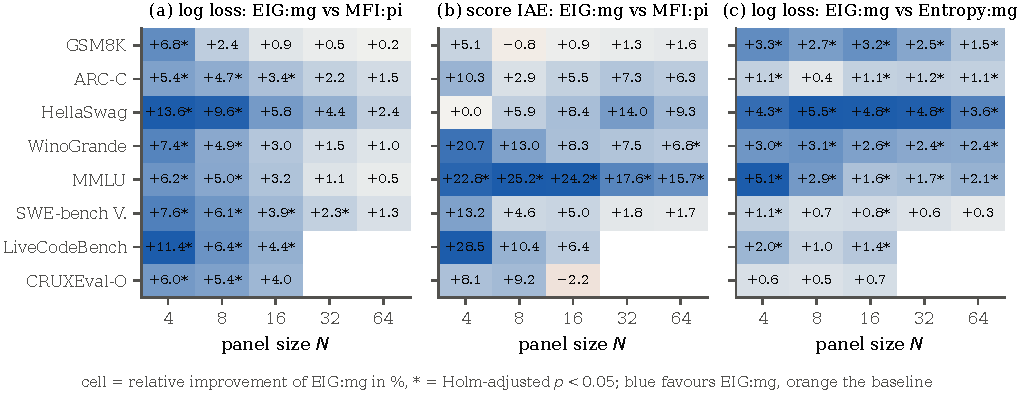
\includegraphics[width=0.92\linewidth]{figures/heatmap_improvement.pdf}
\caption{Study 1: relative improvement (\%) of EOST-M by benchmark and panel size.}
\label{fig:heatmap}
\end{figure}

\paragraph{Learning curves and efficiency.} Every model-based policy starts below the naive
estimator, because the calibrated model predicts the bank before any item is asked
(Figure~\ref{fig:curves-err}). Plug-in policies reduce the error fastest in the first items
(at $t=5$ a plug-in policy is ahead of EOST-M on \EarlyPluginBetter\ of \NCurveBanks\
benchmarks) but then level off: between $t=25$ and $t=100$ the error of plug-in Fisher CAT
falls by a median of \PlateauPi\%, that of EOST-M by \PlateauMg\%, and after 100 items
EOST-M is ahead on \FinalEigBelowMfi\ of \NCurveBanks\ benchmarks---the signature of a bias
floor inherited from the plug-in parameters. At $N=8$, EOST-M matched the score error of 100
uniformly sampled items after a median of \EffItemsMedianNeight\ items (between
\EffItemsMinNeight\ and \EffItemsMaxNeight\ across benchmarks), and after \EffItemsMedianNmax\
with the largest panels. Adaptivity itself contributes: random items scored by the same
marginal model had a mean score IAE of \IAErandmgNeight\ against \IAEeigmgNeight\ for
EOST-M, whose error was significantly lower on \RandIaeFav\ of \RandIaeNB\ benchmarks. Late
in the test, entropy selection under the marginal model catches up, and the crossover comes
later on larger banks (Spearman $\rho=\CrossRho$ over \CrossPoints\ benchmark--panel
combinations, exploratory), the regime change described by Proposition~\ref{prop:evr}; the
score-targeted criterion moved in the predicted direction, but only part of the way. Short
adaptive tests also rank systems well: after 25 items, Kendall's $\tau$ with the true accuracy
had a median of \TauEigTwentyfive\ for EOST-M, \TauMfiTwentyfive\ for plug-in Fisher CAT and
\TauNaiveTwentyfive\ for random items (exploratory).

\begin{figure}[htbp]
\centering
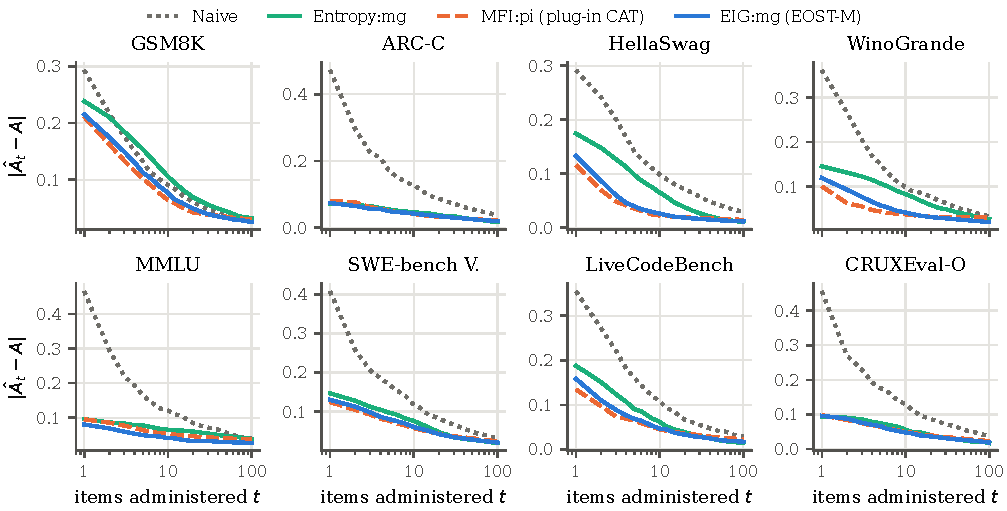
\includegraphics[width=\linewidth]{figures/curves_err_N8.pdf}
\caption{Study 1: absolute score error as items are administered ($N=8$).}
\label{fig:curves-err}
\end{figure}

\paragraph{Uncertainty.} Plug-in posteriors are overconfident (Figure~\ref{fig:coverage}a):
at $N=8$ the 90\% interval of plug-in Fisher CAT covered the score \CovMfipi\ of the time,
EOST-M's \CovEigmg\ and Naive's model-free Wilson interval \CovNaive. Marginalization
removes much of the overconfidence, but no model-based adaptive policy reaches nominal
coverage on real data. On the synthetic banks (Figure~\ref{fig:coverage}b), EOST-M's
coverage at $N=8$ is \SynTwoplEigMgCovNeight\ when the model is well specified,
\SynGuessEigMgCovNeight\ with guessing and \SynTwodimEigMgCovNeight\ with a second ability
dimension, and as the panel grows coverage rises towards the nominal level on synthetic data
but falls on real data: more calibrators sharpen the item posteriors, which helps when the
model is adequate and exposes its misfit when it is not. With known abilities, EOST-M also
had the smallest ability error at $N=8$ on all three synthetic banks
(\SynTwoplEigMgErrNeight, \SynGuessEigMgErrNeight\ and \SynTwodimEigMgErrNeight, against
\SynTwoplMfiPiErrNeight, \SynGuessMfiPiErrNeight\ and \SynTwodimMfiPiErrNeight\ for plug-in
Fisher CAT).

\begin{figure}[htbp]
\centering
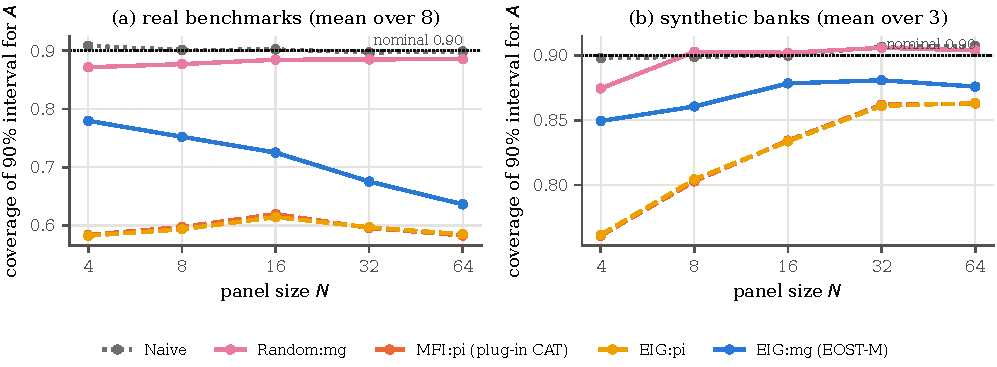
\includegraphics[width=0.88\linewidth]{figures/coverage.pdf}
\caption{Study 1: coverage of the 90\% score interval as a function of the panel size.}
\label{fig:coverage}
\end{figure}

\paragraph{Sensitivity and post hoc probes.} Removing near-duplicate calibrators leaves the
H2 gain essentially unchanged (\SensDedupHTwoNeight\% against
\SensMainDedupBanksHTwoNeight\% on the same benchmarks), but the empirical-Bayes hyperprior
is essential: with a fixed weakly-informative prior the H2 gain falls to
\SensFixedpriorHTwoNeight\% (main analysis: \SensMainHTwoNeight\%), because for an item
that the panel cannot locate the expected response function is essentially the prior
predictive. The one-parameter variant of the frozen plan is degenerate---its likelihood is
invariant to a joint rescaling, and its mode inflates the common discrimination (median
\OneplMedianA)---and is not interpreted. A post hoc variant with
$\log a\sim\mathcal N(0,0.05^2)$ confirms Corollary~\ref{cor:blind}: with one common
discrimination the EIG--entropy difference is \SensOneplregHOneNeight\% under the marginal
model and \SensOneplregHOnePiNeight\% under plug-in parameters, against
\SensMainHOneNeight\% and \SensMainHOnePiNeight\% with item-specific discriminations.

Three post hoc probes, with decision rules recorded before running, then tested a competing
explanation of H2. (i) Posterior-mean plug-in parameters are no remedy (log loss
\PhMfieapLLNeightAbs\% worse than EOST-M), but a regularized Rasch-type plug-in test is a
strong baseline: EOST-M's log loss was lower on all \PhMfioneprLLNeightB\ benchmarks, yet only
by a median of \PhMfioneprLLNeightAbs\% (significant on \PhMfioneprLLNeightFav), and the
Rasch-type intervals were better calibrated (coverage \PhCovMfionepr\ against \PhCovEigmg);
averaging Fisher information over the item posterior selected items as well as EIG (median
difference \PhEfiLLNeightAbs\%), so the optimism of Corollary~\ref{cor:jensen} did not
matter. (ii) Shrinking EOST-M's discriminations towards a common value did not combine the
two remedies: no setting met the criterion fixed in advance (coverage between \ShrMgCovMin\
and \ShrMgCovMax). (iii) The Rasch-type intervals were wider on all \PhThreeWiderBanks\
benchmarks without more accurate estimates, and across all cells coverage was almost a
monotone function of the ratio of interval width to score error (Spearman $\rho=\PhThreeRho$),
a ratio below that of a calibrated Gaussian interval in every cell. The constrained model is
better calibrated because it is less confident, and since random items under the same model
cover \CovRandmg\ of the time, the shortfall arises when adaptive selection meets a
misspecified model. Study~2 tests the Rasch-type competitor under a frozen plan.

\section{Study 2: independent targets and strong competitors}
\label{sec:study2}

Study~2 evaluated \STwoTargetsTotal\ independent targets (\STwoTargetsMin\ to
\STwoTargetsMax\ per benchmark). Table~\ref{tab:study2} lists every frozen decision with the
number of benchmarks on which a Holm-significant difference favours EOST-M or the competitor,
the number on which EOST-M is better, and the median relative improvement (for C3 the
relative difference of the PDM Bayesian CAT, for C5a the range of coverage; C5a, C5b and C6
concern the recalibrated interval, marked by an asterisk). Of the \STwoNHyp\ decisions,
\STwoNSupported\ were supported. Apart from C5b, every superiority contrast favoured EOST-M
on at least seven of the eight benchmarks and no competitor was significantly better on any
benchmark; four of the five superiority hypotheses that were not supported (C2, C4, C7, C8)
missed the threshold by one benchmark. CRUXEval-O, with only \STwoTargetsMin\ independent
clusters, reached significance in no contrast.

\begin{table}[htbp]
\centering\footnotesize
\caption{Study 2: frozen hypotheses at $N=8$ and their decisions.}
\label{tab:study2}
\setlength{\tabcolsep}{3pt}
\begin{tabular}{@{}lllcccl@{}}
\toprule
 & EOST-M versus & Endpoint & Holm sig. & positive & median & Supported \\
\midrule
R2 & plug-in 2PL (MFI:pi) & log loss & 5/0 & 8/8 & $+5.9$ & yes \\
R3 & Naive & score IAE & 6/0 & 8/8 & $+53.9$ & yes \\
R4 & plug-in 2PL (MFI:pi) & $|\mathrm{cov}-0.9|$ & 5/0 & 8/8 & $+41.6$ & yes \\
C1 & Rasch-type plug-in & log loss & 5/0 & 7/8 & $+2.4$ & yes \\
C2 & Rasch-type marginal & log loss & 4/0 & 8/8 & $+1.8$ & no \\
C4 & Random:mg & score IAE & 4/0 & 8/8 & $+21.1$ & no \\
C5b & raw EOST-M interval$^\ast$ & interval score & 0/2 & 4/8 & $+1.0$ & no \\
C6 & Naive (Wilson)$^\ast$ & interval score & 6/0 & 7/8 & $+35.0$ & yes \\
C7 & ATLAS-style 3PL CAT & score IAE & 4/0 & 8/8 & $+26.0$ & no \\
C8 & tinyBenchmarks & error @50 & 4/0 & 8/8 & $+29.6$ & no \\
C9 & MINCE & error @50 & 5/0 & 8/8 & $+44.8$ & yes \\
\midrule
C3 & PDM Bayesian CAT (equivalence) & log loss & \multicolumn{2}{c}{4/8 within $\pm$1\%} & $+0.32$ & no \\
C5a & (coverage in $[0.85,0.95]$)$^\ast$ & coverage & \multicolumn{2}{c}{5/8 banks inside} & 0.81--0.91 & no \\
\bottomrule
\end{tabular}
\end{table}


\paragraph{Replication with independent targets.} The study-1 results held: EOST-M's
held-out log loss was lower than plug-in Fisher CAT's on every benchmark (R2, median
\STwoRTwoMed\%, \STwoRTwoFav\ significant), more so with four calibrators
(\SecRTwoNFourMed\%) than with sixteen (\SecRTwoNSixteenMed\%), and by the same amount for
deterministic (\STwoRTwoDet\%) and aggregate verdicts (\STwoRTwoAgg\%); R3 and R4 were also
supported, and plug-in Fisher CAT's intervals covered the score only \STwoCovmfipi\ of the
time, against \STwoCoveigmg\ for EOST-M.

\paragraph{Integration, constraint and Bayesian CATs.} EOST-M predicted better than the
Rasch-type plug-in test (C1, median \STwoCOneMed\%), more so with sixteen calibrators
(\SecCOneNSixteenMed\%) than with four (\SecCOneNFourMed\%), where a single discrimination
becomes a visible misspecification; the integrated one-parameter model sat in between (C2,
\STwoCTwoMed\%). The two tests had similar score errors (median \SecEostVsRaschIAEMed\%, no
benchmark significant), and the Rasch-type intervals were again better calibrated before
recalibration (\STwoCovmfiOnepr). The PDM Bayesian CAT differed from EOST-M by a median of
\STwoCThreeMed\% in log loss and was within $\pm1\%$ on only \STwoCThreeEq\ benchmarks, so
equivalence (C3) was not supported. Its frozen burn-in proved too short on
\FbDriftFrozenBank, where the mean calibrator ability drifted by a median of
\FbDriftFrozenMax\ during the retained sweeps; with either burn-in (10 or, post hoc, 60
sweeps) it was not significantly different from EOST-M on any benchmark, in log loss or score
error (corrected log loss higher by a median of \FbBmiMed\% with Bayesian maximum information
and \FbEigMed\% with EIG). The exploratory joint fully Bayesian CAT, which
keeps the uncertainty about the location of the calibration shared across items, was the
closest to EOST-M with EIG selection (median \FbjEigMed\%). At $N=4$ the corrected PDM
Bayesian CAT was never significantly better than EOST-M (within $\pm1\%$ on \FbBmiEqNFour\
and \FbEigEqNFour\ benchmarks with the two criteria). With eight calibrators, integrating
their abilities and the hyperprior on top of the item parameters thus made no significant
difference, but equivalence within $\pm1\%$ was not shown.

\paragraph{Adaptivity and benchmark reduction.} All methods used the same eight calibrators;
ATLAS and tinyBenchmarks were designed for hundreds to thousands, so these comparisons concern
the small-panel regime, not the methods in their native settings. Under the same calibrated
model, adaptive selection reduced the score error of random items by a median of
\STwoCFourMed\% (C4, \STwoCFourFav\ benchmarks significant), more with larger panels
(\SecCFourNFourMed\% at $N=4$, \SecCFourNSixteenMed\% at $N=16$). Table~\ref{tab:reduction}
gives the score errors at 25, 50 and 100 items, averaged over targets and benchmarks;
tinyBenchmarks and MINCE choose their items without adapting to the target. After 50 items
EOST-M's error was \STwoCEightMed\% below tinyBenchmarks' gp-IRT (C8) and \STwoCNineMed\%
below MINCE's subset mean (C9, supported), and over the test \STwoCSevenMed\% below the
ATLAS-style CAT's (C7), whose plug-in 3PL parameters and randomesque selection made it the
least accurate model-based policy (coverage \STwoCovatlas). With eight calibrators,
tinyBenchmarks' K-Means cannot always find as many anchors as its budget, because its item
embeddings take only as many values as there are distinct response patterns; an audit
decided before the results were seen showed that restricting C8 to full-budget cells, or
comparing with EOST-M after the number of items tinyBenchmarks actually used, again gave
\TinyFullFav\ significant benchmarks. MINCE's own stopping rule asked for a median of
\STwoMinceNstarMed\ items and then had a score error of \STwoMinceErrNstar\ points, more
than EOST-M after 100 items (\STwoErreigmgHundred).

\begin{table}[htbp]
\centering\footnotesize
\caption{Study 2: absolute score error (points) after 25, 50 and 100 items at $N=8$.}
\label{tab:reduction}
\begin{tabular}{@{}lccc@{}}
\toprule
Method & 25 items & 50 items & 100 items \\
\midrule
EOST-M (EIG:mg) & 3.39 & 2.81 & 2.13 \\
ATLAS-style 3PL CAT & 4.46 & 4.20 & 3.79 \\
Random:mg & 4.78 & 3.34 & 2.42 \\
tinyBenchmarks gp-IRT & 4.96 & 4.39 & 4.49 \\
tinyBenchmarks p-IRT & 4.69 & 3.92 & 3.31 \\
tinyBenchmarks anchors & 6.23 & 5.62 & 5.37 \\
MINCE subset mean & 6.71 & 4.69 & 3.19 \\
Naive (Wilson) & 7.05 & 4.88 & 3.26 \\
\bottomrule
\end{tabular}
\end{table}


\paragraph{Calibrated uncertainty.} Model-based intervals remained too narrow: EOST-M
covered the score \STwoCoveigmg\ of the time, the PDM Bayesian CAT \FbBmiCov, the Rasch-type
test \STwoCovmfiOnepr\ and plug-in Fisher CAT \STwoCovmfipi, whereas Random:mg reached
\STwoCovrandommg\ and Naive's Wilson interval \STwoCovnaive. Recalibration raised EOST-M's
coverage to \STwoCoveigmgRR, inside $[0.85,0.95]$ on \STwoCFiveaIn\ benchmarks, one short of
the criterion (C5a), and did not improve the interval score (C5b; significantly worse on
HellaSwag and WinoGrande): the wider intervals cost about as much as the misses they removed.
The recalibrated intervals had a much better interval score than Naive's Wilson intervals
(C6, median \STwoCSixMed\%) because they were much narrower (mean width \STwoWidtheigmgRR\
against \STwoWidthnaive). Recalibration brought the Rasch-type test inside the band on all
eight benchmarks, but with intervals about twice as wide (\STwoWidthmfiOneprRR). It needs
calibrators as pseudo-targets and helped more as the panel grew (coverage
\STwoCovEostRNFour, \STwoCovEostRNEight\ and \STwoCovEostRNSixteen\ at $N=4$, 8 and 16), and
mixing one uniformly drawn item in four into the adaptive test raised coverage only to
\STwoCovmixmg.

\paragraph{Temporal validation and the hyperprior.} On the \TempTargets\ SWE-bench
Verified submissions of the latest quarter, calibrated only on earlier submissions,
\TempNSig\ of the \TempNTests\ frozen contrasts favoured EOST-M at a Holm-adjusted $p<0.05$
within the component and none favoured a competitor; EOST-M's log loss was \TempRTwoMed\% lower than plug-in
Fisher CAT's and \TempCOneMed\% lower than the Rasch-type test's. Because the empirical-Bayes
hyperprior is essential and estimated from the same panel, it was checked post hoc and varied
under the frozen plan. Resampling items moves the hyperparameters by at most
\EBItemsSdMaxEight\ (standard deviation, $N=8$), whereas resampling calibrators moves them
about as much as the variation between panels: the hyperprior reflects which systems are in
the panel, not noise in the items. Prior predictive checks reproduce the spread of the
items' proportions correct, but the share of items with identical panel verdicts only on
average, and real systems agree with each other less, item by item, than a unidimensional
2PL with independent items implies (mean item--rest correlation \PPCRestObs\ observed,
\PPCRestSim\ simulated): the response model is misspecified in its dependence structure, one
reason why model-based intervals are too narrow. A cross-fitted hyperprior, estimated for
each item on the other half of the items, left EOST-M's log loss unchanged (median
\SecXfVsEostMedAbs\%), and Student-$t$ hyperpriors made it slightly worse
(\SecTpVsEostMedAbs\%): the gain of EOST-M does not come from fitting the prior to the items
it is applied to.

\section{Robustness of the study-2 conclusions}
\label{sec:robust}

A second review asked whether the response-derived clusters favour EOST-M, whether the
Bayesian CATs were estimated with enough MCMC, and whether the effects generalize across
benchmarks. Three follow-ups (RF1--RF3), whose plans and decision rules were written before
they were run, answer these questions, together with exploratory extensions (RF2b--RF2d,
RF3b) planned in the same way; none changes a frozen decision.

\paragraph{Clusters that never see the target's responses (RF1).} The strict clusters use
residuals computed from every system's responses, the target's included, and excluding the
calibrators that resemble a target could make its panel harder to calibrate. Keeping the
frozen targets, holdouts and seeds, we rebuilt the panels from heuristic families alone,
from residuals computed on the other benchmarks, and with residual thresholds from 0.4 to 0.7.
Under every rule, R2 and C1 kept their frozen median improvements (\RobRTwoMedMin\% and
\RobCOneMedMin\%), R2 remained positive on all eight benchmarks with \RobRTwoFavRange\
significant, and C1 positive on seven with \RobCOneFavRange\ significant and none against:
the robustness criterion fixed in advance was \RobRuleMet.

\paragraph{MCMC quality of the Bayesian CATs (RF2--RF2d).} We ran the frozen sampler with
four long chains on \ConvPanels\ panels and computed rank-normalized split $\hat R$ and bulk
effective sample sizes \citep{vehtari2021rank}. The overall location converged ($\hat R<1.05$
on \ConvLocRhatFive\% of panels), but $\sigma_b$, $\mu_a$ and $\sigma_a$ did not
($\hat R<1.05$ on at most \ConvHypRhatFiveMax\%): multiplying all abilities and difficulties
by a constant and dividing the discriminations by it leaves the likelihood unchanged, so with
eight calibrators only their $\mathcal N(0,1)$ prior fixes the scale of the calibration, and
the frozen sampler has no move along this ridge. Under the rule fixed in advance the study-2
statement about the Bayesian CATs was \ConvRule: the long chains changed the cell-level log
loss by a median of \ConvLongAbsVsSixtyMin--\ConvLongAbsVsSixtyMax\% relative to a burn-in of 60,
more than the 0.5\% allowed, while the long-chain arms differed from EOST-M by a median of \ConvLongVsEostMin\
to \ConvLongVsEostMax\%, with the benchmarks split. Exploratory samplers then added a
Metropolis--Hastings move along the scale ridge with the item parameters summed out (RF2b, a
partially collapsed Gibbs sampler with a discrete form of parameter expansion;
\citealp{vandyk2008partially,liu1999parameter}) and sampled the model of
Lemma~\ref{lem:exact} exactly, with collapsed moves for the hyperparameters, the scale and the
location (RF2d). RF2d came much closer to convergence (medians of $\hat R$ at most
\ExtRhatMedMaxAll, largest value \ExtRhatMaxAll\ against \ConvHypRhatMax\ for the frozen
sampler) but reached $\hat R<1.05$ on only \ExtRhatFiveMin\% of panels for its slowest
quantity, short of the 90\% fixed in advance, so a fully converged comparator was not
obtained. Across all \AllBayesNArms\ combinations of Bayesian arm and sampler, the median
difference from EOST-M in held-out log loss stayed within $\pm$\AllBayesVsEostMaxAbs\%, with
the benchmarks split: the comparison did not move as the sampler improved, which makes an
artefact of the frozen chain unlikely. The RF2d arms covered the score as often as EOST-M
on the same cells (\ExtCovMin--\ExtCovMax\ against \ExtEostCov), and their score error was lower by a median of
\ExtIaeGainMin--\ExtIaeGainMax\% over cells but on only \ExtIaeBanksMin--\ExtIaeBanksMax\ of
8 benchmarks, a possible advantage that 48 cells cannot establish.

\paragraph{Effects across benchmarks (RF3, RF3b).} The frozen rule requires significance on
five of eight benchmarks after a Holm correction over 88 tests, so an effect can favour
EOST-M everywhere and still be declared not supported. A secondary random-effects
meta-analysis that treats the benchmarks as independent found pooled improvements excluding
zero for \MetaNExclZero\ of the 11 superiority hypotheses, including the
\MetaNExclZeroUnsup\ near misses (\MetaUnsupList). Five benchmarks, however, share the same
395 Open LLM Leaderboard systems. Counting them as one source (RF3b: \MetaSrcK\ sources, with
a bootstrap over the shared systems), \MetaSrcNExclZero\ of the 11 intervals excluded zero
(\MetaSrcExclList), and of the near misses only \MetaSrcUnsupKeptList\ kept an interval above
zero; the dependence through shared systems was small (median correlation \MetaSrcR), and the
loss comes from having four heterogeneous sources. Most effects point the same way across
benchmarks; the analysis does not show that they generalize to a new one.

\section{What adaptive evaluation costs}
\label{sec:cost}

Adaptive testing saves items only after a calibration panel has answered the whole bank.
Counting one administered item as the unit of cost, evaluating $M$ new systems costs $MI$
with the full bank of $I$ items and $NI+MT$ with a fresh panel of $N$ calibrators and tests of
$T$ items, so adaptive testing pays off once $M>NI/(I-T)$. Table~\ref{tab:cost} gives, for
$N=8$ and $T=100$, this break-even point (between \CostBreakFullMin\ and \CostBreakFullMax\
new systems), the number of items with which EOST-M matches the score error of 100 items
sampled uniformly and scored by the sample mean (Naive) or by the same calibrated model
(Random:mg), and the break-even point against Naive. Uniform subsampling needs no panel, so
it is the fairer comparison: EOST-M saves about \CostSaveNaive\ items per system against it
and breaks even after a median of \CostBreakNaiveMed\ new systems (from \CostBreakNaiveMin\
to \CostBreakNaiveMax). When the calibrators' results already exist---public leaderboards or
earlier internal evaluations---the panel is free and adaptive testing is cheaper from the
first system; when items are expensive, as in agentic benchmarks, the per-system saving
dominates quickly. Calibrating a panel and running a 100-item test take seconds on one CPU
core.

\begin{table}[htbp]
\centering\footnotesize
\caption{Cost of adaptive evaluation with a fresh panel of eight calibrators.}
\label{tab:cost}
\begin{tabular}{@{}lrrrrr@{}}
\toprule
 & & break-even vs & items to match & break-even vs & items to match \\
Benchmark & $I$ & full evaluation & Naive@100 & Naive & Random:mg@100 \\
\midrule
GSM8K & 1319 & 8.7 & 70 & 352 & 80 \\
ARC-C & 1172 & 8.7 & 20 & 117 & 90 \\
HellaSwag & 2000 & 8.4 & 8 & 174 & 25 \\
WinoGrande & 1267 & 8.7 & 20 & 127 & 60 \\
MMLU & 2000 & 8.4 & 15 & 188 & 100 \\
SWE-bench V. & 500 & 10.0 & 40 & 67 & 70 \\
LiveCodeBench & 1055 & 8.8 & 25 & 113 & 60 \\
CRUXEval-O & 800 & 9.1 & 25 & 85 & 60 \\
\bottomrule
\end{tabular}
\end{table}


\section{Discussion}
\label{sec:discussion}

\paragraph{Small-panel calibration uncertainty is the problem.} With four or eight
calibrators a large fraction of items is answered identically by every calibrator, so their
difficulty is located only by the prior. Plug-in testing treats these
poorly located parameters as known: Fisher selection credits such items with information
they do not carry, the plug-in posterior becomes overconfident, and the predicted outcomes of
the unobserved items inherit the parameter errors---the bias floor of
Figure~\ref{fig:curves-err}. The expected response function caps the information of such
items (Proposition~\ref{prop:cap}) and predicts their outcomes with the uncertainty they
actually have. Both effects fade as the panel grows (Figure~\ref{fig:heatmap}): for the very
large panels of recent work \citep{li2026atlas}, plug-in Fisher information is an adequate
approximation; for new, private or expensive benchmarks, self-generated item pools, or the
panels of four to eight systems that a single laboratory can afford, it is not.

\paragraph{Integrating and constraining are two remedies.} Integrating the item posterior
(EOST-M) predicted better than constraining the discriminations to a common value (C1), more
so with sixteen calibrators, whereas the constrained model's intervals were better calibrated
because they are wider, not because its estimates are more accurate. A small panel must
therefore not be trusted with item-specific discriminations: integrating their uncertainty is
preferable when prediction and score accuracy matter most, and constraining them gives a
simpler and more conservative test.

\paragraph{Why not always use a fully Bayesian adaptive test?} It is the principled answer
to calibration uncertainty, and \citet{fink2025accounting} found it the most accurate
correction with hundreds of calibration responses per item. With eight calibrators it did not
help measurably, although equivalence was not shown either. By Lemma~\ref{lem:exact}, EOST-M
is the fully Bayesian model with the calibrators' abilities and the hyperprior held fixed; in
this regime what matters, as far as our data can tell, is the item-level uncertainty that
both integrate. A fully Bayesian test also needs a Markov chain per panel, whose tuning is a
source of error in its own right: our frozen burn-in was too short on some banks, and even an
exact sampler with collapsed moves did not meet our convergence criterion. EOST-M is the
simpler default. Two leads remain open: the near-converged sampler suggests a possible
advantage of Bayesian integration for estimating the score, and panel-level uncertainty may
matter more when the calibrators' abilities are poorly determined, as with short banks.

\paragraph{The criterion matters less than first hypothesized.} The pilot program and
study~1 agree on the direction of the original thesis---EIG learns more about competence than
predictive entropy---but bound its size: under the same calibration-marginal model the gain
on held-out prediction is small, and the information criteria are practically
interchangeable (a descriptive comparison; the failure of H1 is not a test of equivalence).
Corollary~\ref{cor:blind} explains why: entropy and information disagree only through the
spread of discriminations among items with similar success probabilities, which the expected
response function shrinks, and with a common discrimination the difference vanishes. For the
bank score, Proposition~\ref{prop:evr} shows that uncertainty sampling becomes the right
one-step criterion once competence is pinned down relative to the unobserved bank, and the
score-error curves show both regimes. What an adaptive test for LLMs must get right is the
treatment of calibration uncertainty, not the choice among information criteria.

\paragraph{Honest uncertainty.} None of the four remedies tried in study~2---integrating
the calibrators' abilities, leave-one-calibrator-out recalibration, mixing random items into
the test, recalibrating a constrained model---gave nominal coverage with intervals as narrow as
EOST-M's. The coverage decomposition and the prior predictive checks locate the problem where
adaptive selection meets a model that is misspecified in the dependence among real systems'
verdicts. Recalibration is not yet a validated remedy: it raised coverage, but neither frozen
criterion for it was met, and on the well-specified synthetic bank it moved coverage away
from the nominal level. Practitioners should report model-based intervals with the panel size
and their expected under-coverage, and use a Wilson interval from uniformly sampled items when
nominal coverage matters more than width.

\paragraph{Adaptive testing or benchmark reduction?} With a handful of calibrators,
tinyBenchmarks, ATLAS-style CAT and MINCE rely on quantities that a small panel cannot
determine well. In this regime our evidence favours adaptive selection under calibration
uncertainty, in the same direction on every benchmark but conclusively by the frozen
criterion only against MINCE; with large panels the differences should shrink.

\paragraph{Limitations.} (i) All evidence replays recorded verdicts: replay is exact for the
recorded data but omits the sampling variability of stochastic decoding, and the protocol we
release for live evaluation could not be run in our environment; the temporal validation
approximates, but does not replace, a prospective deployment. (ii) LiveCodeBench and
CRUXEval-O carry binarized pass rates; graded responses would need another measurement model.
(iii) The unidimensional 2PL is misspecified in the dependence among real systems' verdicts.
(iv) Strict clusters are a heuristic that may miss distant relatives such as distilled models,
although R2 and C1 did not depend on how they were built. (v) Recalibration rests on very
few pseudo-targets, without a finite-sample guarantee. (vi) A fully converged Bayesian
comparator, for instance by Hamiltonian Monte Carlo, remains to be run. (vii) The analysis
plans were frozen by hashing and committing them, without an external time stamp. (viii) Item
exposure was not controlled; an adaptive benchmark that serves the same informative items to
every model would accelerate their contamination \citep{wainer2000cat}. (ix) Joint MAP
calibration made the planned one-parameter sensitivity analysis degenerate; marginal maximum
likelihood would avoid this. (x) Self-generated items were studied only in a historical
pilot. (xi) The cross-benchmark meta-analysis is secondary and limited by shared systems.

\paragraph{Recommendations.} With a small calibration panel: (1) do not plug in
item-specific discriminations calibrated on fewer than a few dozen systems, but integrate their
uncertainty with an empirical-Bayes prior, or constrain them when a simple, conservative test
matters more than accuracy; (2) select by any information criterion computed from the marginal
model, and let the score-targeted criterion take over late in the test when the estimand is
the score; (3) prefer the calibration-marginal model to the Bayesian treatments of the
calibrators that we ran, which made no significant difference; (4) report model-based
intervals with the panel size and their expected under-coverage; (5) exclude the target's whole
cluster from its panel and analyse with clusters as units; (6) count the panel in the cost.

\section{Conclusion}
\label{sec:conclusion}

Adaptive testing can make LLM evaluation cheaper, but with the small calibration panels of
new, private or expensive benchmarks it works only if the uncertainty of the item calibration
is taken seriously. Integrating it through expected response functions with an empirical-Bayes
prior is simple, exact given the calibrators, and caps the information of items that a small
panel cannot locate. Under frozen analysis plans, this predicted held-out verdicts better than
plug-in Fisher-information testing and a regularized Rasch-type test, estimated scores more
accurately than uniform subsampling and MINCE, was ahead of random items, ATLAS-style testing
and tinyBenchmarks on every benchmark without meeting the frozen criterion for these
comparisons, and was not significantly different from Bayesian CATs that also integrate the
calibrators' abilities, without being shown equivalent. The thesis that information rather than entropy should be maximized
holds in sign but is modest once uncertainty is integrated. The open problem is honest
uncertainty: model-based intervals remain too narrow, and recalibration from the panel improved
coverage only at the price of width.

\section*{Data and code availability}
The analysis code, the Docker environment, both frozen analysis plans, the scripts that
rebuild every response matrix from its pinned public source, all experimental artifacts with
their SHA-256 hashes, and the manuscript sources, including an extended version of this
article with every secondary table and figure, are publicly available at
\url{https://github.com/mesellemahmed/eost}. Response matrices derived from MIT-licensed
sources are distributed with the code; the others are rebuilt from their pinned sources by
the provided scripts and checked against the published hashes.

\section*{Declaration of competing interest}
The authors declare that they have no known competing financial interests or personal
relationships that could have appeared to influence the work reported in this paper.


\vskip 0.2in
\bibliography{refs}

\end{document}
